    \documentclass[
        fleqn,
        usenatbib,
        referee,
    ]{mnras}
    \usepackage{
        amsmath,
        amssymb,
        newtxtext,
        newtxmath,
        graphicx,
        ae, aecompl,
        booktabs,
        caption,
        subcaption,
    }
    \usepackage[T1]{fontenc}
    \captionsetup{compatibility=false}

    \newcommand*{\rd}[2]{\frac{\mathrm{d}#1}{\mathrm{d}#2}}
    \newcommand*{\rtd}[2]{\frac{\mathrm{d}^2#1}{\mathrm{d}#2^2}}
    \newcommand*{\pd}[2]{\frac{\partial#1}{\partial#2}}
    \newcommand*{\md}[2]{\frac{\mathrm{D}#1}{\mathrm{D}#2}}
    \newcommand*{\at}[1]{\left.#1\right|}
    \newcommand*{\abs}[1]{\left|#1\right|}
    \newcommand*{\ev}[1]{\langle#1\rangle}
    \newcommand*{\bm}[1]{\boldsymbol{\mathbf{#1}}}
    \newcommand*{\uv}[1]{\hat{\bm{#1}}}
    \newcommand*{\p}[1]{\left(#1\right)}
    \newcommand*{\s}[1]{\left[#1\right]}
    \newcommand*{\z}[1]{\left\{#1\right\}}
    \DeclareMathOperator*{\argmin}{argmin}
    \DeclareMathOperator*{\argmax}{argmax}
    \DeclareMathOperator*{\med}{med}

\title[Analytical Exoplanet Obliquities]{Analytical Predictions of Exoplanet
Obliquities Generated by Planet-Disk Interactions}
\author[Y. Su and D. Lai]{
Yubo Su$^1$,
Dong Lai$^1$
\\
$^1$ Cornell Center for Astrophysics and Planetary Science, Department of
Astronomy, Cornell University, Ithaca, NY 14853, USA
}

\date{Accepted XXX\@. Received YYY\@; in original form ZZZ}

\pubyear{2019}

\begin{document}\label{firstpage}
\pagerange{\pageref{firstpage}--\pageref{lastpage}}
\maketitle

\begin{abstract}
    Large planetary spin-orbit misalignments (obliquities) are thought to play a
    key role in some planets' atmospheric circulation and tidal heating. A
    promising avenue to generate high obliquities is via spin-orbit resonances,
    where the spin and orbital precession frequencies of the planet become and
    remain commensurate as the system evolves. One such proposed mechanism
    involves a dissipating protoplanetary disk driving orbital precession of an
    interior planet \citep{millholland_disk}. This previous work is limited to
    small initial misalignment angles between the spin axis of the planet and
    orbital axis of the massive disk. In the present paper, this scenario is
    analytically characterized and extended to arbitrary misalignment angles. It
    is shown that (i) under adiabatic evolution, final planetary obliquities
    bifurcate into distinct tracks governed by interactions with the resonance,
    while (ii) under non-adiabatic evolution, a broad range of obliquities can
    be excited. Analytical formulae are provided for most interesting regimes of
    parameter space.
\end{abstract}

\begin{keywords}
planet--star interactions % chktex 8
\end{keywords}

\section{Introduction}\label{s:intro}

Substantial planetary obliquities, defined as the angle between a planet's spin
and orbital axes, have been proposed in many exoplanetary systems. They lie at
the heart of the obliquity tides mechanism of radius enhancement in hot Jupiters
\citep{winn_otides, fabrycky_otides, millholland_wasp12b}. They have also been
invoked to explain peculiar thermal phase curves in hot Jupiters \citep[see
e.g.][]{millholland_signatures, ohno_infer_obl}. While exoplanet obliquities
have yet to be directly detected, techniques have been proposed to constrain
them \citep[see e.g.][]{schwarz_infer_obl, rauscher_infer_obl}.

Many mechanisms have been proposed to generate large planetary obliquities.
Giant impacts are traditionally used to generate the large obliquities of the
solar system ice giants \citep{original_gi, morbidelli_gi}. More recently,
obliquity excitations have been achieved via \emph{spin-orbit resonances}, where
the spin and orbital precession frequencies of the planet become and remain
commensurate as the system evolves (sometimes called \emph{resonance
advection}). Spin-orbit resonances have been studied extensively in solar system
dynamics as \emph{Cassini States} and are responsible for the significant
nonzero obliquities of both Jupiter ($3.1^\circ$) and Saturn ($26.7^\circ$)
\citep{colombo1966, henrard1987, ward2004I, ward_jupiter}. Recent work has
attempted to apply this mechanism to the ice giants as well
\citep{hamilton_tilting_ice}.

Producing exoplanet obliquities via spin-orbit resonances was the subject of
\citet{millholland_disk}, where a dissipating protoplanetary disk causes
resonance capture and advection. In their work, they begin with a planet whose
spin is nearly aligned with the angular momentum vector of the protoplanetary
disk. After the disk dissipates, the resulting planetary obliquity is generally
substantial, reaching $90^\circ$ for what they characterize as adiabatic
resonance crossings.

However, their study was limited to small initial misalignment angles between
the spin vector of the planet and the orbital angular momentum of the
protoplanetary disk. Such an assumption is intuitive, since the planet forms
from the disk, but prospects for it to be violated exist. In particular, giant
and planetesimal impacts are expected to be abundant during planet formation and
may perturb the spin axis of the protoplanet from its primordial value
\citep{yalinewich2019atmospheric, schlichting2015atmospheric}. Furthermore, the
abundance of compact multi-planet systems provides support for possible
scattering between close-in, newly-formed planets \citep{usp_compact1,
usp_review}. It is conceivable that such processes could generate significant
spin-disk misalignment within the lifetime of the disk.

In our work, we provide an analytical framework for understanding the final
planetary obliquity for arbitrary initial spin-disk misalignment angles. Our
analytical work and independent numerical simulations are in agreement with
\citet{millholland_disk} but provide a more complete characterization of
possible behavior. While we solve a specific dynamics problem, our analysis
is general and has a wide range of applicability to general resonance
encounters.

The paper is organized as follows. In Section~\ref{s:eq}, we review relevant
spin-orbit dynamics and present the equations studied in the rest of the paper.
In Sections~\ref{s:ad} and~\ref{s:nonad}, we study the evolution of the system
when the disk either dissipates adiabatically or non-adiabatically respectively.
Exhaustive yet simple analytical arguments are able to explain completely the
numerical results in both limits. We discuss potential consequences in
Section~\ref{s:disc}. Our primary physical results consist of
Fig.~\ref{fig:ad_ensemble} in the adiabatic limit and
Fig.~\ref{fig:3_ensemble_05_15} in the non-adiabatic limit. Longer mathematical
calculations are relegated to the appendicies, including a leading-order
estimate of final planetary obliquities given small initial spin-disk
misalignment angles in Appendix~\ref{s:ad_approx}.

\section{Theory}\label{s:eq}

\subsection{Equations of Motion}

We consider a star of mass $M_\star$ hosting an oblate planet of mass $M_{\rm
p}$, radius $R_{\rm p}$, at semimajor axis $a_{\rm p}$, and with spin angular
frequency $\Omega_{\rm p}$, and a protoplanetary disk of mass $M_{\rm d}$. For
simplicity, we treat the disk as a ring of radius $r_d$, but it is simple to
generalize to a disk with finite extent \citep[see][]{millholland_disk}.
Denote $\bm{S}$ the spin angular momentum and $\bm{L}$ the orbital angular
momentum of the planet, and $\bm{L}_{\rm d}$ the angular momentum of the disk.
The corresponding unit vectors are $\uv{s} \equiv \bm{S} / S$,
$\uv{l} \equiv \bm{L} / L$, and $\uv{l}_{\rm d} \equiv \bm{L}_{\rm
d} / L_d$.

We assume $S \ll L \ll L_{\rm d}$, so $\uv{l}_{\rm d}$ is approximately
constant and $\uv{l}$ experiences negligible backreaction torque from
$\uv{s}$. The equations of motion for $\uv{s}$ and $\uv{l}$
are
\begin{align}
    \rd{\uv{s}}{t} &= \omega_{\rm sl} \p{\uv{s} \cdot \uv{l}}
            \p{\uv{s} \times \uv{l}}
        \equiv \alpha \p{\uv{s} \cdot \uv{l}}
            \p{\uv{s} \times \uv{l}},\label{eq:dsdt}\\
    \rd{\uv{l}}{t} &= \omega_{\rm ld}\p{\uv{l} \cdot \uv{l}_{\rm d}}
            \p{\uv{l} \times \uv{l}_{\rm d}}
        \equiv -g\p{\uv{l} \times \uv{l}_{\rm d}},
            \label{eq:dldt}
\end{align}
where
\begin{align}
    \omega_{\rm sl} &= \frac{3k_{\rm qp}}{2k_{\rm p}} \frac{M_\star}{m_{\rm
        p}} \p{\frac{R_{\rm p}}{a_{\rm p}}}^3 \Omega_{\rm p},\label{eq:wsl}\\
    \omega_{\rm ld} &= \frac{3M_{\rm d}}{4M_\star}\p{\frac{a_{\rm
        p}}{r_{\rm d}}}^3 n .\label{eq:wld}
\end{align}
% = 1/(152600 yr) (kp = 6kqp, Mstar = msun, mp = mJ, Rp = RJ, ap = AU, Wp = 2pi
% / (10 days))
% = 1 / (573362 yr) (Md/Mstar = 0.01, ap/rd = 1/30)
In Eq.~\eqref{eq:wsl}, $k_{\rm qp}$ and $k_{\rm p}$ are related to the planet's
rotation-induced quadrupole moment and moment of inertia respectively
\citep[see][]{lai2018}, and $n \equiv \sqrt{GM_\star/a_{\rm p}^3}$ is the
planet's orbital mean motion. The three angles formed by the three vectors are
denoted
\begin{align}
    \theta &\equiv \arccos \p{\uv{s} \cdot \uv{l}},\\
    \theta_{\rm sd} &\equiv \arccos \p{\uv{s} \cdot \uv{l}_{\rm d}},\\
    I &\equiv \arccos \p{\uv{l} \cdot \uv{l}_{\rm d}}.
\end{align}
Following standard notation \citep[e.g.][]{colombo1966,peale1969,ward_jupiter},
we have defined $\alpha \equiv \omega_{\rm sl}$ and $g \equiv -\omega_{\rm
ld}\cos I$.

We can combine Eqs.~\eqref{eq:dsdt} and~\eqref{eq:dldt} into a single equation
by transforming into a frame rotating about $\uv{l}_{\rm d}$ with
frequency $(-g)$. In this frame, $\uv{l}_{\rm d}$ and $\uv{l}$ are fixed, and
$\uv{s}$ evolves as:
\begin{equation}
    \p{\rd{\uv{s}}{t}}_{\rm rot} = \alpha \p{\uv{s} \cdot \uv{l}}
            \p{\uv{s} \times \uv{l}}
        + g\p{\uv{s} \times \uv{l}_{\rm d}}.\label{eq:dsdt_rot}
\end{equation}

We define the frequency ratio $\eta$ and dimensionless time $\tau$ as
\begin{align}
    \eta \equiv{}& -\frac{g}{\alpha}\nonumber\\
        ={}& 3.75 \p{\frac{k_{\rm p}}{6k_{\rm qp}}}
            \p{\frac{m_{\rm p}}{0.001 M_\odot}}
            \p{\frac{R_{\rm p}}{R_{\rm J}}}^{-3}\nonumber\\
        &\times \p{\frac{M_{\rm d}}{0.01 M_{\odot}}}
            \p{\frac{a_{\rm p}}{1\;\mathrm{AU}}}^{9/2}
            \p{\frac{r_{\rm d}}{30 \;\mathrm{AU}}}^{-3}
            \p{\frac{M_\star}{1M_{\odot}}}^{-3/2}
            \cos I,\label{eq:eta}\\
    \tau \equiv{}& \alpha t.
\end{align}
In Eq.~\eqref{eq:eta}, we have introduced the fiducial values of variable
parameters for the appciation considered in this paper. Eq.~\eqref{eq:dsdt_rot}
then becomes
\begin{equation}
    \p{\rd{\uv{s}}{\tau}}_{\rm rot} = \p{\uv{s} \cdot \uv{l}}
            \p{\uv{s} \times \uv{l}}
        - \eta\p{\uv{s} \times \uv{l}_{\rm d}}. \label{eq:dsdt_base}
\end{equation}

Throughout this paper, we consider $\alpha$ constant, but allow $g$ to vary in
time. In the dispersing disk scenario of \citet{millholland_disk}, $\abs{g}$
decreases in time due to the decreasing disk mass. We consider a simple
exponential decay model
\begin{equation}
    M_{\rm d}(t) = M_{\rm d}(0)e^{-t/t_{\rm d}},\label{eq:dmd_dt}
\end{equation}
with $t_{\rm d}$ constant. This implies $\mathrm{d}\eta / \mathrm{d}t = -\eta /
t_{\rm d}$. In dimensionless units, we have
\begin{equation}
    \rd{\eta}{\tau} = -\epsilon \eta\label{eq:deta_dt},
\end{equation}
where
\begin{align}
    \epsilon \equiv{}& \frac{1}{\alpha t_{\rm d}},\label{eq:eps_def}\\
        ={}& 0.015 \p{\frac{k_{\rm p}}{6k_{\rm qp}}}
            \p{\frac{m_{\rm p}/M_\star}{0.001}}
            \p{\frac{a_{\rm p}}{1\;\mathrm{AU}}}^3\nonumber\\
        &\times \p{\frac{R_{\rm p}}{R_{\rm J}}}^{-3}
            \p{\frac{\Omega_{\rm p}}{2\pi/\p{10\;\mathrm{days}}}}
            \p{\frac{t_{\rm d}}{10\;\mathrm{Myr}}}^{-1}.
\end{align}
Eqs.~\eqref{eq:dsdt_base} and~\eqref{eq:deta_dt} together constitute our system
of study.

In the next two subsections, we summarize the theoretical background relevant to
our analysis of the evolution of the system.

\subsection{Cassini States}\label{ss:cs}

Spin states satisfying $\p{\rd{\uv{s}}{t}}_{\rm rot} = 0$ are referred to as
\emph{Cassini States} (CSs). They require that $\uv{s}$, $\uv{l}$, and
$\uv{l}_{\rm d}$ be coplanar. There are either two or four CSs, depending
on the values of $\eta$. They are specified by the obliquity $\theta$ and the
precessional phase of $\uv{s}$ around $\uv{l}$, denoted by $\phi$. Following
the standard convention and nomenclature (see Fig.~\ref{fig:cs_locs}), CSs 1, 3, 4
have $\phi = 0$ and $\theta < 0$, corresponding to $\uv{s}$ and $\uv{l}_{\rm
d}$ being on opposite sides of $\uv{l}$, while CS2 has $\phi = \pi$ and $\theta
> 0$, corresponding to $\uv{s}$ and $\uv{l}_{\rm d}$ being on the same side of
$\uv{l}$. When $\eta < \eta_{\rm c}$, where
\begin{equation}
    \eta_{\rm c} \equiv \p{\sin^{2/3}I + \cos^{2/3}I}^{-3/2},\label{eq:etac}
\end{equation}
all four CSs exist, and when $\eta > \eta_{\rm c}$, only CSs 2, 3 exist. The CS
obliquities as a function of $\eta$ are shown in Fig.~\ref{fig:cs_locs}.
\begin{figure}
    \centering
    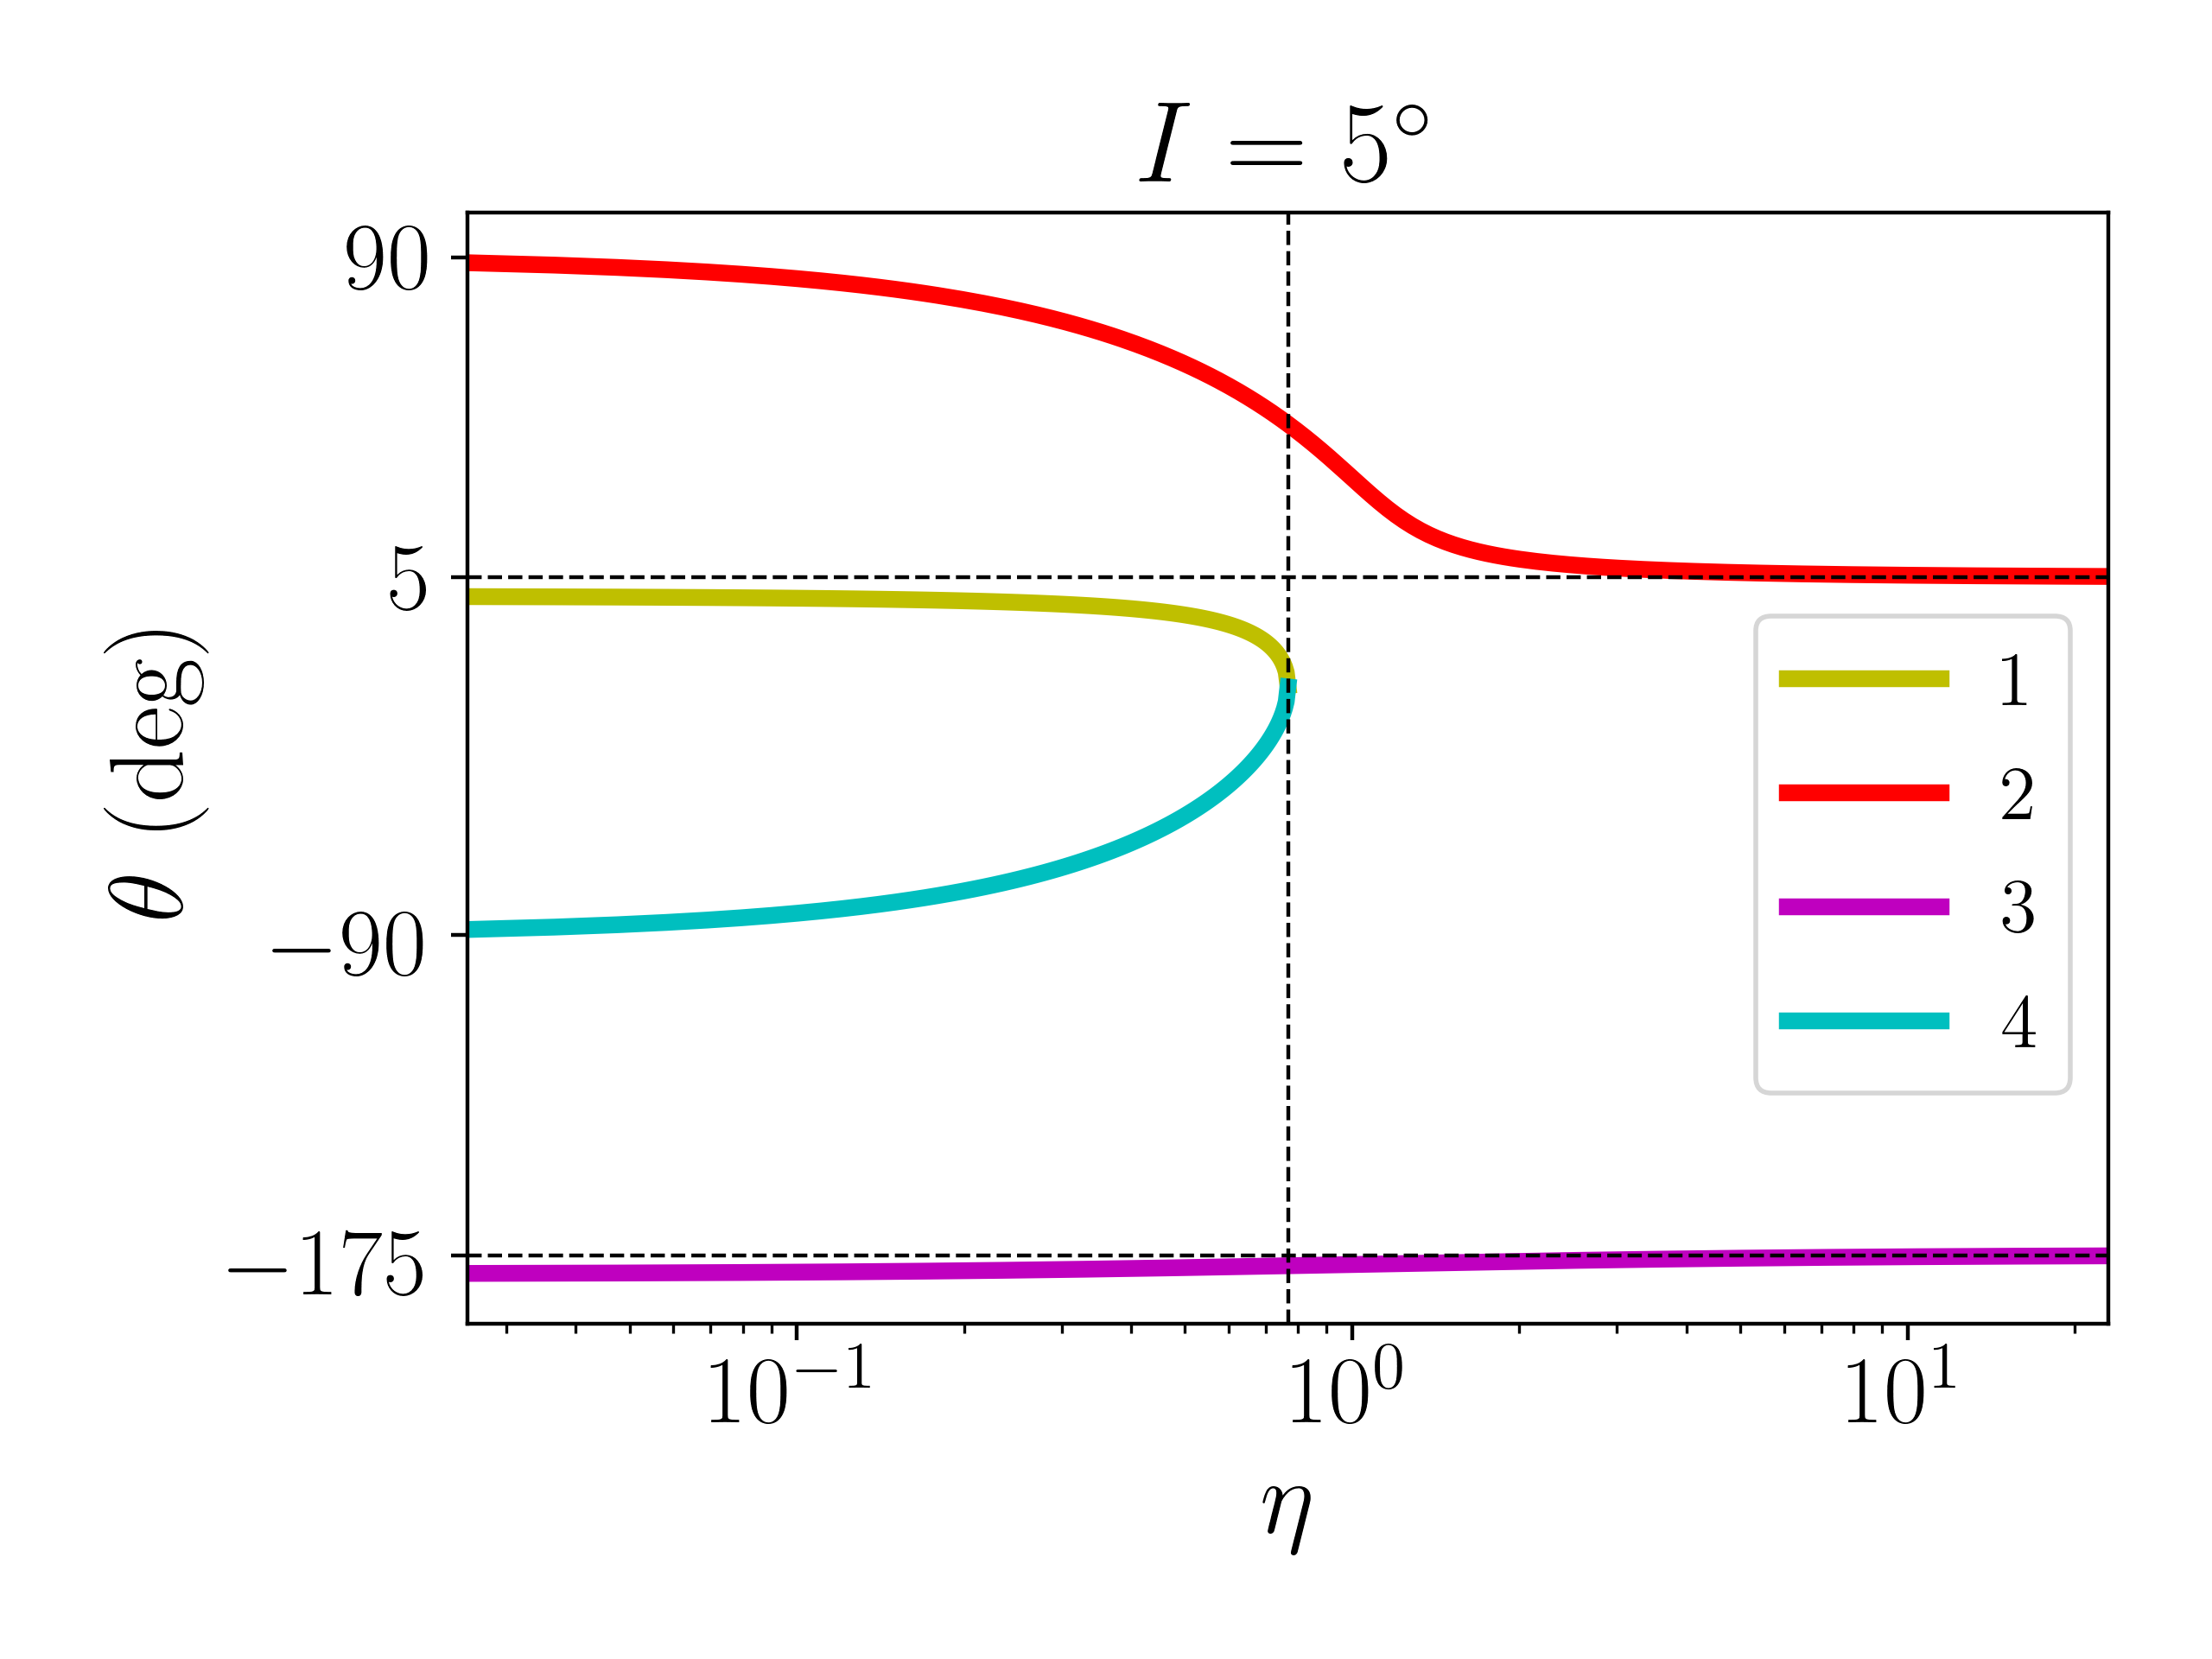
\includegraphics[width=0.5\textwidth]{../initial/99_misc/2_cs_locs.png}
    \caption{Cassini state obliquities as a function of $\eta$ for $I =
    5^\circ$. Note that $\theta \in [-\pi, \pi]$ is the traditional definition
    of the polar angle. The vertical dashed line indicates $\eta_{\rm c}$ ($=
    0.766$ for $I = 5^\circ$), where CS1 and CS4 merge and annihilate, and the
    horizontal dashed lines indicate $\theta = I$ and $I - 180^\circ$, the
    asymptotic values for CSs 2 and 3 for $\eta \gg \eta_{\rm
    c}$.}\label{fig:cs_locs}
\end{figure}

Of the four CSs, 1, 2, 3 are stable while 4 is unstable.
Appendix~\ref{s:local_dynamics} gives the libration frequencies and growth rates
respectively near these CSs.

\subsection{Separatrix}

The Hamiltonian (in the rotating frame) of the system is
\begin{align}
    \mathcal{H} &= -\frac{1}{2}\p{\uv{s} \cdot \uv{l}}^2
            + \eta \p{\uv{s} \cdot \uv{l}_{\rm d}}\nonumber\\
        &= -\frac{1}{2}\cos^2\theta
            + \eta \p{\cos \theta \cos I - \sin I \sin \theta \cos \phi}
                \label{eq:H}.
\end{align}
Trajectories in the phase space $\p{\phi, \cos \theta}$ satisfy $H = $ constant
(see Fig.~\ref{fig:eq_1contours}).

When $\eta < \eta_{\rm c}$, CS4 exists and is a saddle point. The two
trajectories originating and ending at CS4 are the only two infinite-period
orbits in the phase space. Together, these two critical trajectories are
referred to as the \emph{separatrix} and divide phase space into three zones. In
Fig.~\ref{fig:eq_1contours}, we show the separatrix, the three zones, and their
relations to the CSs. Note that trajectories in zone II librate about CS2
while those in zones I and III circulate.
\begin{figure*}
    \centering
    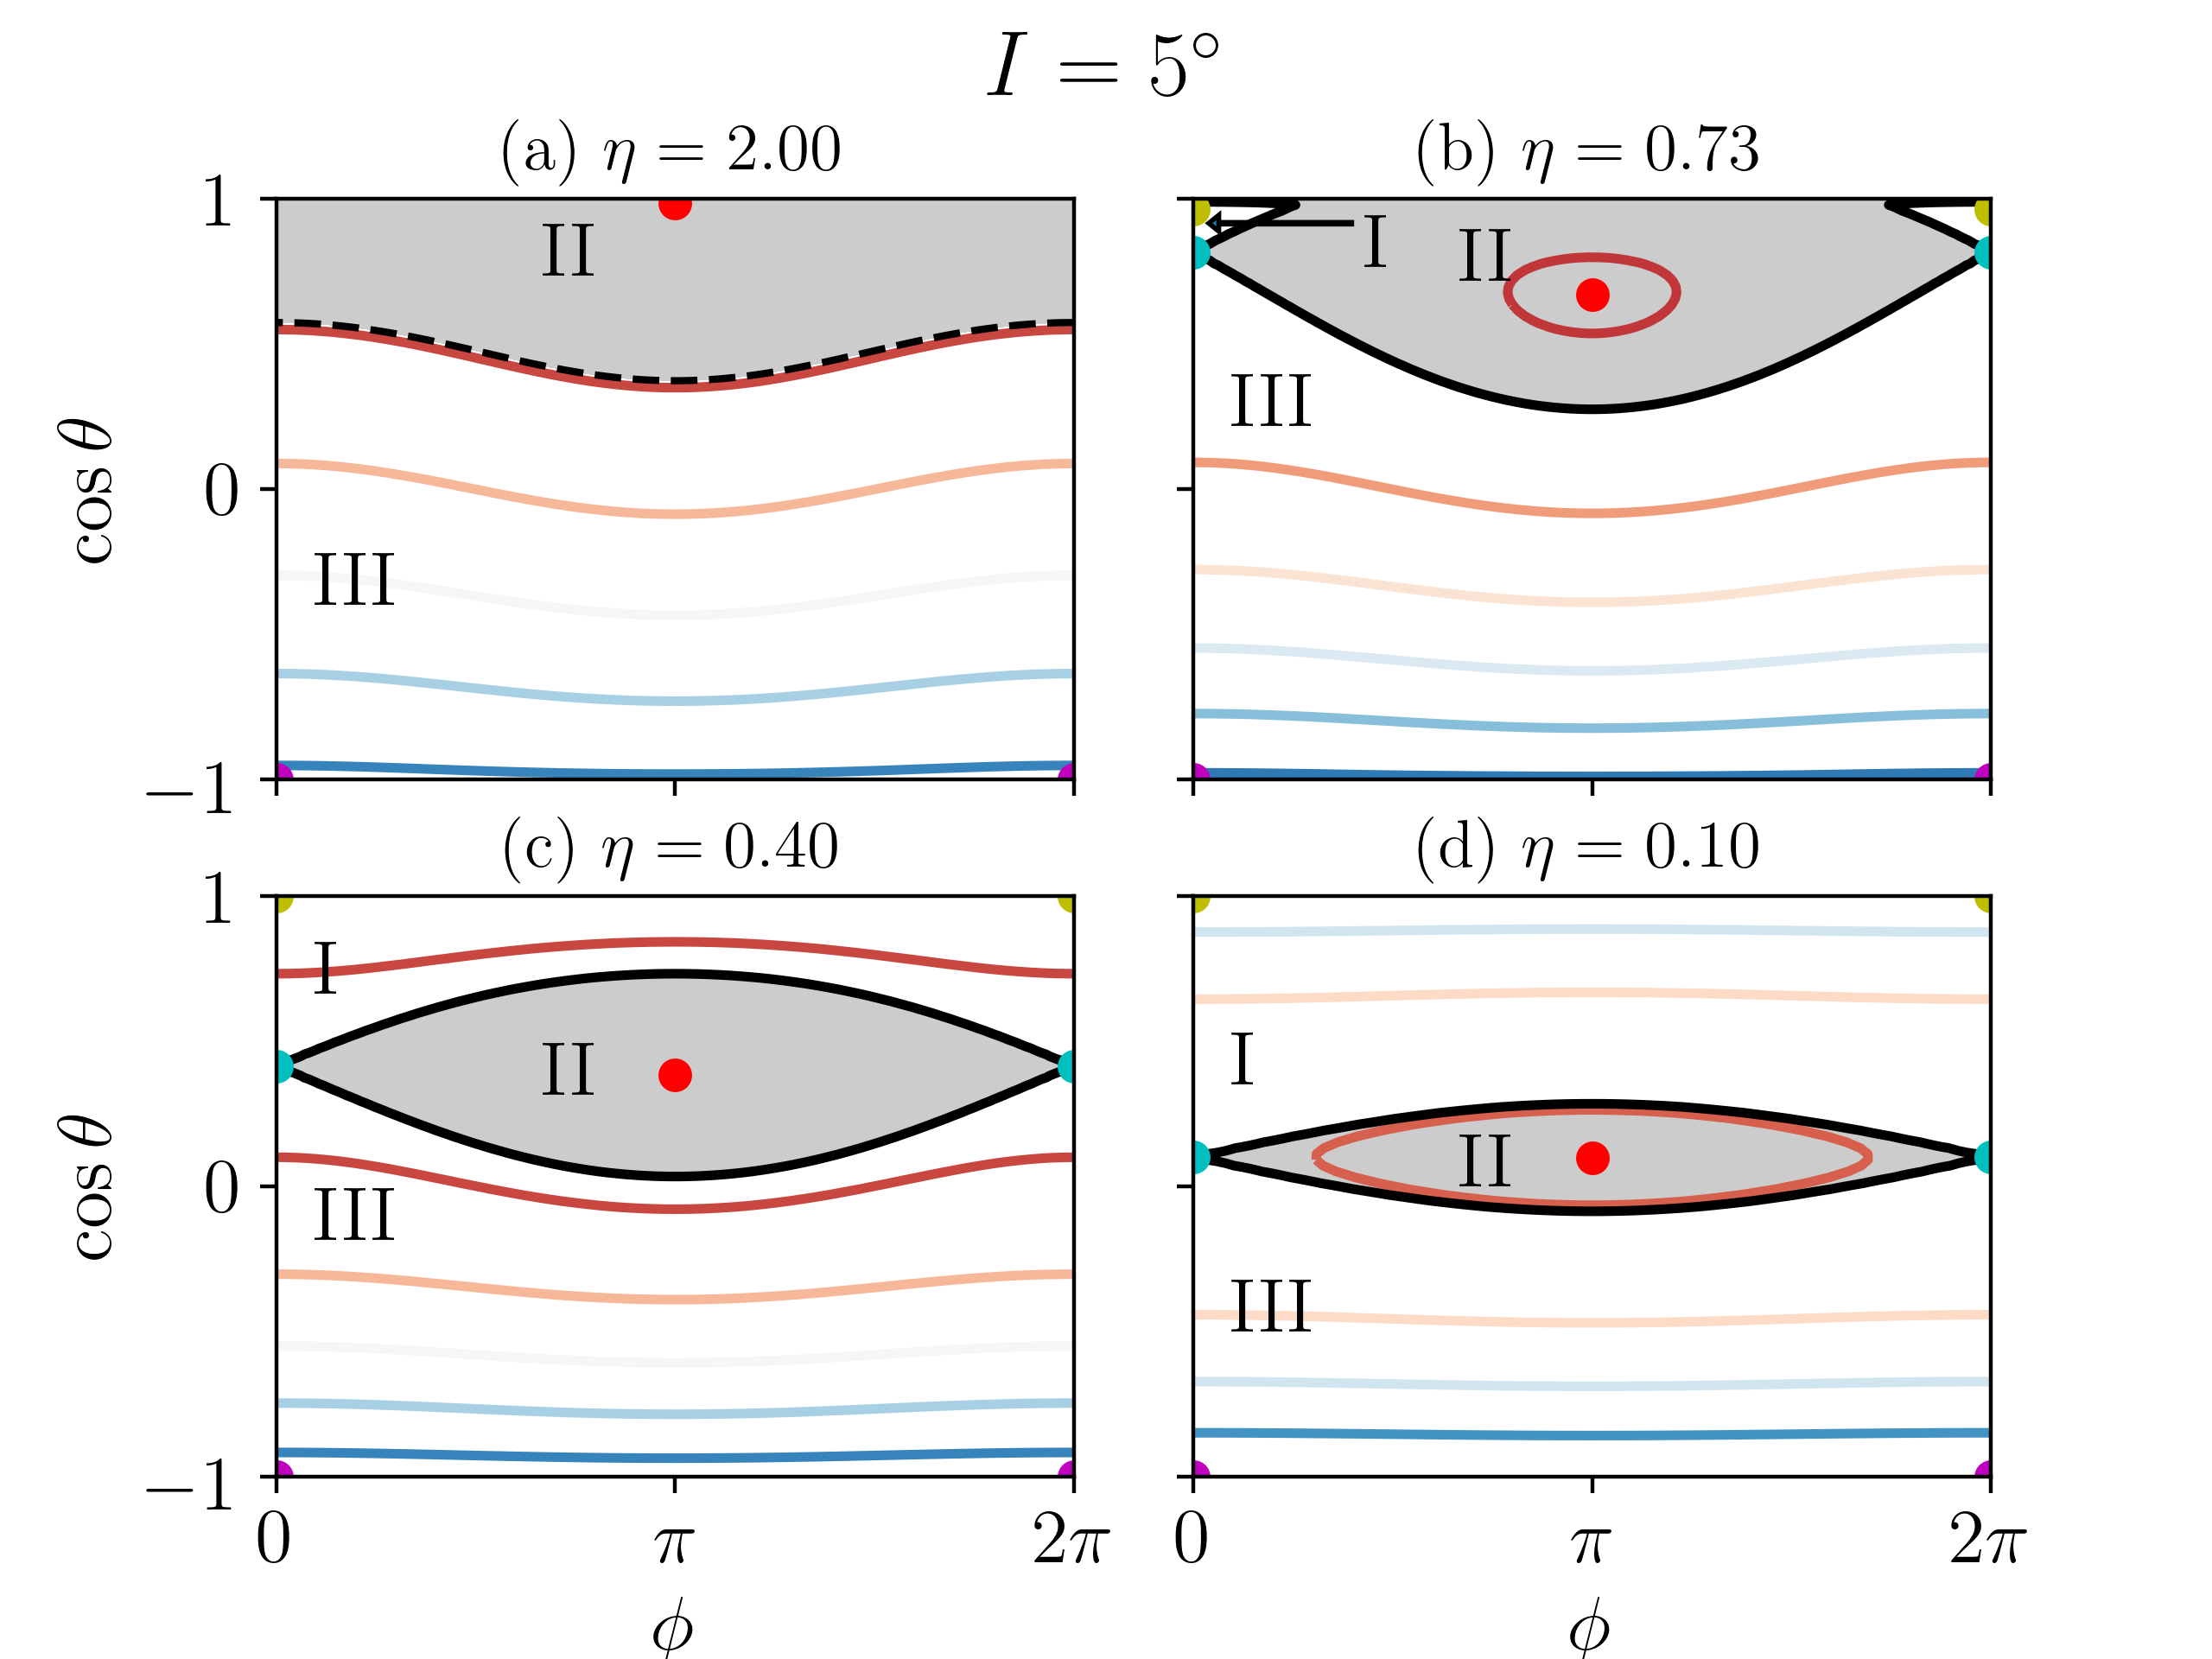
\includegraphics[width=0.8\textwidth]{../initial/0_eta/1contours_flip.png}
    \caption{Level curves plot of $\mathcal{H}\p{\phi, \cos \theta}$
    [Eq.~\eqref{eq:H}] for $I = 5^\circ$, where warmer colors denote more
    positive values. The black solid line is the separatrix, which only exists
    for $\eta < \eta_{\rm c} = 0.766$. The three zones (I, II, III), divided by
    the separatrix, are labeled. The Cassini states are denoted by filled
    circles and have the same colors as in Fig.~\ref{fig:cs_locs}. The interior
    of the separatrix, shaded in grey, is formally only defined for $\eta <
    \eta_{\rm c}$, but we may identify the points in phase space that flow into
    zone II when evolved forward in time (decreasing $\eta$ adiabatically); this
    is the shaded region in the top left panel, bounded by the black dotted
    line.}\label{fig:eq_1contours}
\end{figure*}

Since $\p{\phi, \cos \theta}$ form a set of canonical variables, the integral
$\oint \cos \theta\;\mathrm{d}\phi$ along a trajectory is an adiabatic invariant
(see Section~\ref{s:ad}). The unsigned areas $\p{\abs{\int \cos \theta
\;\mathrm{d}\phi}}$ of the three zones (as defined in
Fig.~\ref{fig:eq_1contours}) can be computed analytically
\citep{henrard1987,ward2004I}. Define
\begin{subequations}
    \begin{align}
        z_0 &= \eta\cos I, &
        \chi &= \sqrt{-\frac{\tan^3\theta_4}{\tan I} - 1},\\
        \rho &= \chi \frac{\sin^2 \theta_4\cos \theta_4}{
            \chi^2 \cos^2\theta_4 + 1},&
        T &= 2\chi \frac{\cos \theta_4}{
            \chi^2 \cos^2\theta_4 - 1}.
    \end{align}
\end{subequations}
The areas for $\eta < \eta_{\rm c}$ are given by
\begin{subequations}\label{se:area_ward}
    \begin{align}
        A_{\rm I} &= 2\pi\p{1 - z_0} - \frac{A_2}{2},\\
        A_{\rm II} &= 8\rho + 4\arctan T - 8z_0 \arctan \frac{1}{\chi},\\
        A_{\rm III} &= 2\pi\p{1 + z_0} - \frac{A_2}{2}.
    \end{align}
\end{subequations}
These are plotted as a function of $\eta$ in Fig.~\ref{fig:eq_areas}. Note that
the zones are not formally defined for $\eta > \eta_{\rm c}$ since the
separatrix disappears, but a natural extension exists: evolve an initial phase
space point $p$ under adiabatic decrease of $\eta$ until the separatrix appears
at $\eta = \eta_{\rm c}$, then identify $p$ with the zone it is in at $\eta_{\rm
c}$. Since phase space area is conserved under adiabatic evolution, this
extension implies $A_{\rm i}\p{\eta > \eta_{\rm c}} = A_{\rm i}(\eta_{\rm c})$.
The boundary between these extended zones is denoted by the dashed black line in
the top left panel of Fig.~\ref{fig:eq_1contours}, where otherwise no separatrix
exists.
\begin{figure}
    \centering
    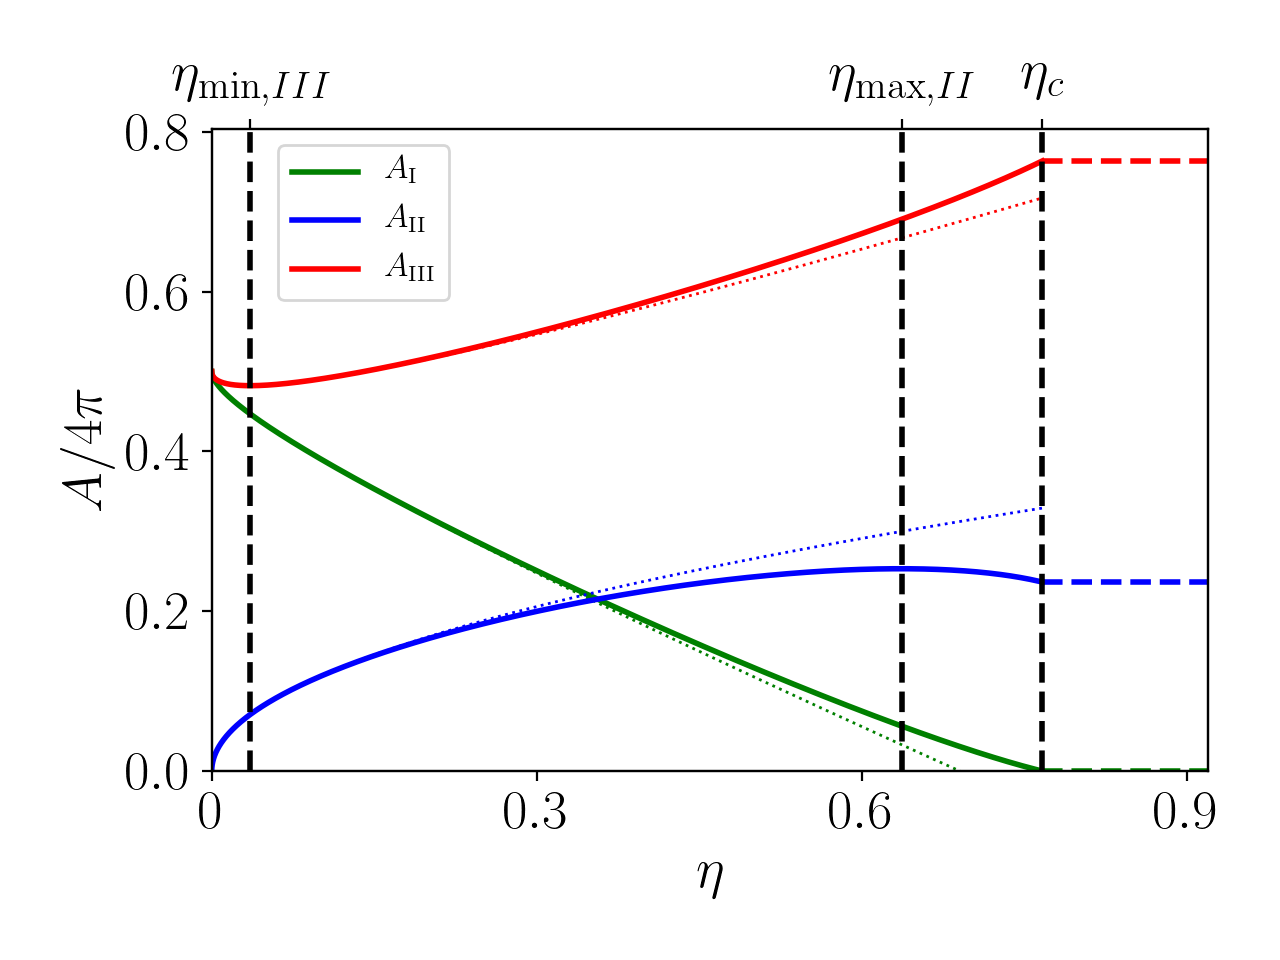
\includegraphics[width=0.5\textwidth]{../initial/99_misc/1_areas.png}
    \caption{The solid lines show the fractional areas of each of the zones
    $A_{\rm i}(\eta) / 4\pi$ as given by Eqs.~\eqref{se:area_ward}. The colored
    dashed lines correspond to small $\eta$ approximations used in
    Appendix~\ref{s:ad_approx}. The colored dashed lines for $\eta > \eta_{\rm
    c}$ are the effective values of $A_{\rm II}, A_{\rm III}$ for $\eta >
    \eta_{\rm c}$, denoting the points that would flow into either area under
    adiabatic decrease of $\eta$ from $\eta > \eta_{\rm c}$. The vertical black
    dashed lines correspond to $\eta = \eta_{\rm c}$ [Eq.\eqref{eq:etac}] and
    the values of $\eta$ for which $A_{\rm II}$ is maximized ($\eta_{\rm \max,
    II}$) and for which $A_{\rm III}$ is minimized ($\eta_{\rm \min, III}$,
    Eq.~\eqref{eq:eta_minIII}). The horizontal black dashed line illustrates the
    fraction of phase space occupied by zone II at separatrix appearance.
    }\label{fig:eq_areas}
\end{figure}

\section{Adiabatic Evolution}\label{s:ad}

In this section, we study the evolution of the planetary obliquity $\theta$ when
the parameter $\eta$ (or the disk mass $M_{\rm d}$; see Eqs.~\eqref{eq:eta}
and~\eqref{eq:deta_dt}) decreases sufficiently slowly that the evolution is
adiabatic. Strictly speaking, this requires the disk evolution timescale $t_{\rm
d}$ [Eq.~\eqref{eq:dmd_dt}] be much larger than all timesccales of the dynamical
system governed by the Hamiltonian [Eq.~\eqref{eq:H}]. This is of course not
possible in all cases, as the motion along the separatrix has an infinite
period.

In practice, as $\eta$ evolves, the system only crosses the separatrix once or
twice, while it spends many orbits inside one of the three zones and far from
the separatrix. Thus, a \emph{weak adiabaticity criterion} is that the variation
timescale of $\eta$ be slower than all circulation/libration timescales near the
equilibria/fixed points. If this criterion is satisfied, then the system will
evolve adiabatically for most of its evolution save one or two separatrix
crossings.

As shown in Appendix~\ref{ss:eigens}, libration about CS2 is slower than that
about CS1 or CS3. As such, it is the slowest characteristic frequency in the
system. The weak adiabaticity criterion can be recast as requiring that $\eta$
vary more slowly than this libration frequency
\citep[see][]{ward2004II,millholland_disk}, i.e.\ $t_{\rm d}^{-1} \lesssim
\omega_{\rm lib} / 2\pi$. In terms of the dimensionless parameter $\epsilon$
[Eq.~\eqref{eq:eps_def}], this adiabaticity condition is
\begin{equation}
    \epsilon = \frac{1}{\alpha t_{\rm d}}
        \lesssim \frac{1}{2\pi}\sqrt{\eta\sin I \sin \theta_2
            \p{1 + \eta \sin I \csc^3 \theta_2}},
            \label{eq:ad_constr}
\end{equation}
where $\theta_2$ is the obliquity at CS2. This formula differs from that given
in \citet{millholland_disk}, where the $\csc^3\theta_2$ term is neglected and
the square root is missing.

For $I = 5^\circ$, $\eta \sim \eta_{\rm c}$ Eq.~\eqref{eq:ad_constr} gives $\epsilon
\lesssim 0.085$. Since our criterion is only a weak condition for diabaticity,
we use $\epsilon = 3 \times 10^{-4}$ in our ``adiabatic'' simulations below
(Section~\ref{ss:ad_ensemble}). We explore the consequences of nonadiabatic
evolution in Section~\ref{s:nonad}.

\subsection{Adiabatic Evolution Outcomes}\label{ss:ad_ensemble}

We consider the evolution of a system with arbitrary initial spin-disk
misalignment angle $\theta_{\rm sd, i}$ and initial $\eta_{\rm i} \gg 1$. We are
interested in the final spin obliquities $\theta_{\rm f}$ after $\eta$ gradually
decreases to $\eta_{\rm f} \ll 1$ (i.e.\ after the disk has dissipated to a
negligible mass). Note that when $\eta_{\rm i} \gg 1$, $\uv{l}$ precesses
around $\uv{l}_{\rm d}$ much faster than the spin-orbit precession
($\abs{\omega_{\rm ld}} \gg \abs{\omega_{\rm sl}}$), and the spin obliquity
$\theta$ varies rapidly. So it is more appropriate to use $\theta_{\rm sd}$
rather than $\theta$ to specify the initial spin orientation. We explore the
entire range $\theta_{\rm sd, i} \in [0, \pi]$ and choose $\epsilon = 3 \times
10^{-4}$ so that the system evolves almost adiabatically (see above).

To obtain the distribution of the final obliquities $\theta_{\rm f}$, we evenly
sample $101$ values of $\theta_{\rm sd, i}$, and for each $\theta_{\rm sd, i}$
value, we pick $101$ orientations of $\uv{s}$ approximately from the ring of
initial conditions having angular distance $\theta_{\rm sd, i}$ to $\uv{l}_{\rm
d}$%
%
\footnote{The procedure we adopted for choosing the initial conditions is the
natural extension of this for finite $\eta_{\rm i}$. Note that the center of
libration of $\uv{s}$ is CS2, which, since $\eta_{\rm i}$ is finite, is
different from $\uv{l}_{\rm d}$. Furthermore, the libration is not exactly
circular. As a result, the libration trajectories for initial conditions on the
circular ring of points having angular distance $\theta_{\rm sd, i}$ from
$\uv{l}_{\rm d}$ are not the same and will each enclose slightly different
initial phase space areas $A_{\rm i}$. Since our analytical theory assumes exact
conservation of phase space area $A_{\rm i}$ derived from $\theta_{\rm sd, i}$
(see Section~\ref{ss:zone_transitions}), this discrepancy introduces an extra
deviation from the analytical prediction. To guarantee all points for a
particular $\theta_{\rm sd, i}$ have the same $A_{\rm i}$, we instead choose
initial conditions on the libration cycle going through $\p{\theta_2 +
\theta_{\rm sd, i}, \phi_2}$ [where $\p{\theta_2, \phi_2}$ are the coordinates
of CS2]. This ensures that all initial conditions for a given $\theta_{\rm sd,
i}$ enclose the same initial $A_{\rm i}$. Note that as $\eta_{\rm i} \to
\infty$, CS2 becomes coincident with $\uv{l}_{\rm d}$ and the libration cycle
becomes exactly circular, recovering the procedure given in the text.}.
%
To be concrete, we choose $\eta_{\rm i} = 10\eta_{\rm c}$ where $\eta_{\rm c}$
is given by Eq.~\eqref{eq:etac} and evolve Eqs.~\eqref{eq:dsdt_base}
and~\eqref{eq:deta_dt} until $\eta$ reaches its final value $10^{-5}$. At such a
small $\eta$, $\uv{s}$ is strongly coupled to $\uv{l}$ and the final obliquity
$\theta_{\rm f}$ is frozen. The mapping between $\theta_{\rm sd, i}$ and
$\theta_{\rm f}$ is our primary result, and is shown for $I = 5^\circ, 10^\circ,
20^\circ$ in Figs.~\ref{fig:ad_ensemble},~\ref{fig:3_ensemble_10_35},
and~\ref{fig:3_ensemble_20_35} respectively. The blue dots represent the results
of the numerical calculation. The colored tracks are calculated
semi-analytically using the method discussed in the following subsection.

\begin{figure}
    \centering
    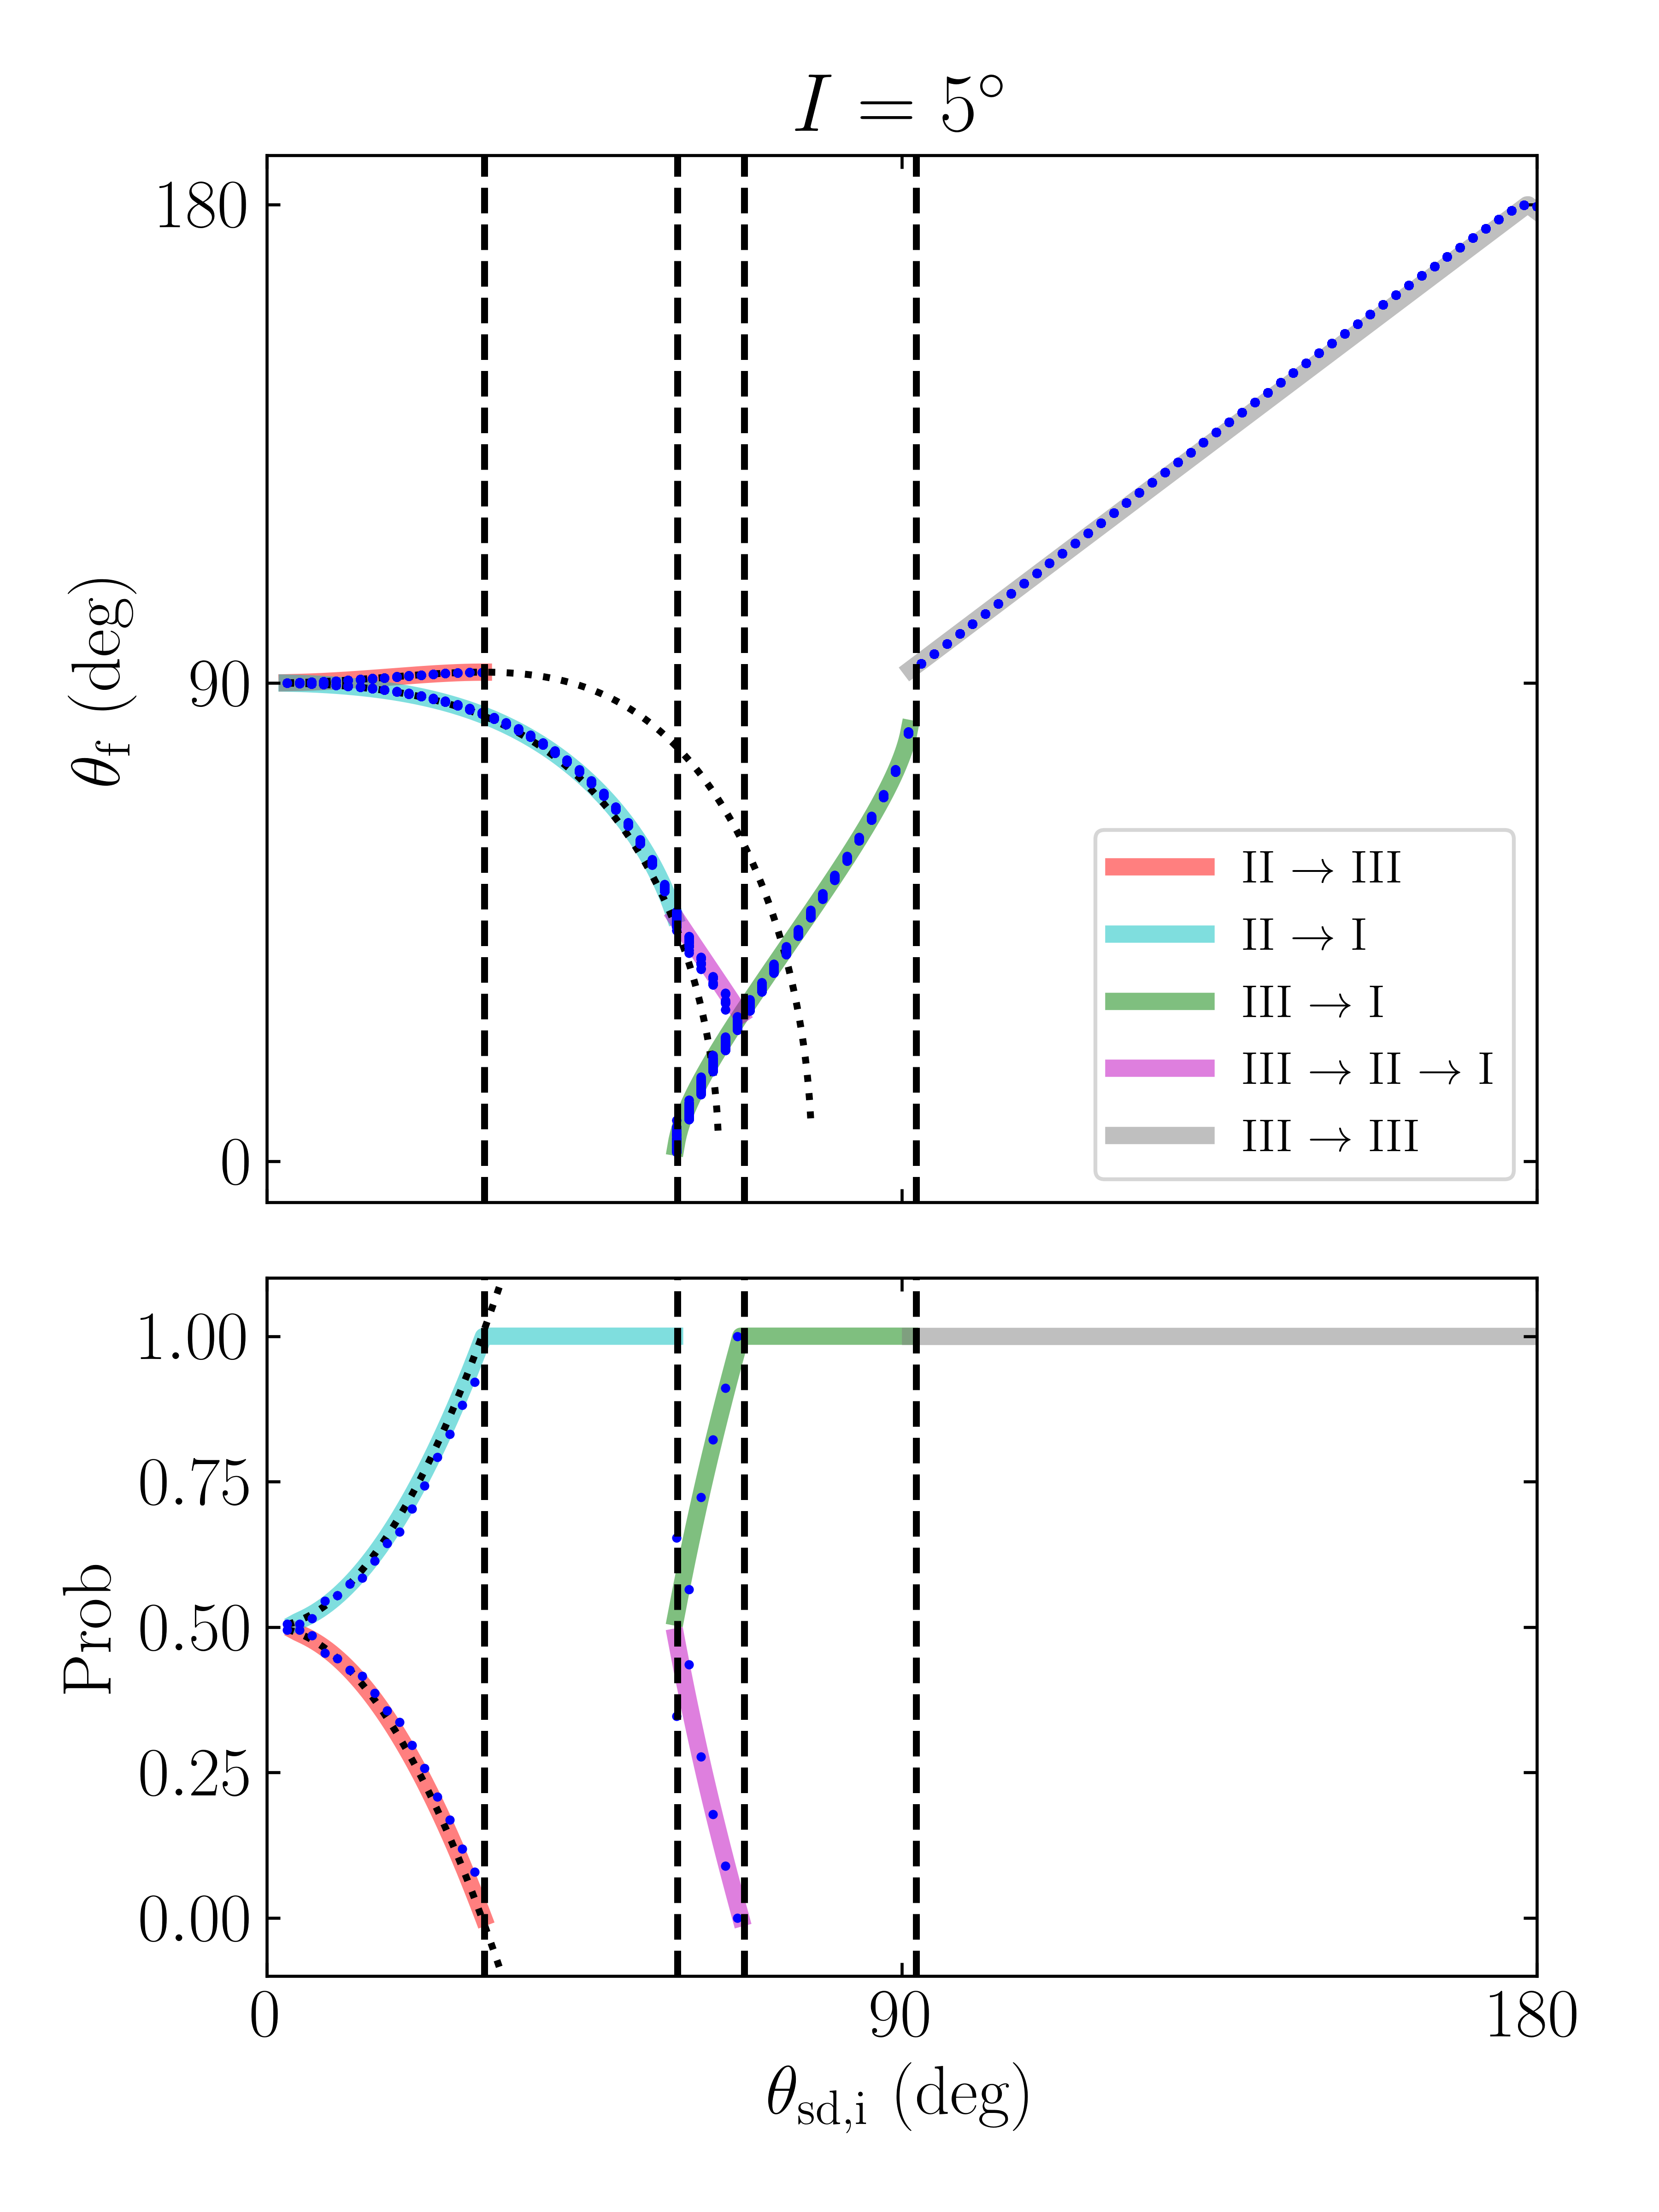
\includegraphics[width=0.5\textwidth]{../initial/2_toy2/3_ensemble_05_35.png}
    \caption{Top: Shown are the final spin obliquity $\theta_{\rm f}$ as a
    function of the initial spin-disk misalignment angle $\theta_{\rm sd, i}$
    for systems evolving from initial $\eta_{\rm i} \gg 1$ to $\eta_{\rm f} \ll
    1$. The blue dots are results of numerical calculations
    (Section~\ref{ss:ad_ensemble}), and the colored tracks are semi-analytical
    results (Section~\ref{ss:zone_transitions}). The black dotted lines
    represent analytical approximations valid in the small-$\theta_{\rm sd, i}$
    limit (see Appendix~\ref{s:ad_approx}). Bottom: Shown are the probabilities
    of different outcomes. Where a particular $\theta_{\rm sd, i}$ corresponds
    to multiple tracks, the system evolves probabilistically. The track that a
    particular system evolves along in a numerical simulation can be measured by
    examining its final obliquity. The dots represent the inferred probabilities
    from measured final obliquities in our simulations, while the colored tracks
    denote the semi-analytic probability of the system evolving along each
    track. There are five regimes of $\theta_{\rm sd, i}$ values for which
    different tracks are accessible. Semi-analytical calculations of the
    boundaries of these regimes are denoted via the vertical dashed black lines
    (see Section~\ref{ss:zone_transitions}).}\label{fig:ad_ensemble}
\end{figure}
\begin{figure}
    \centering
    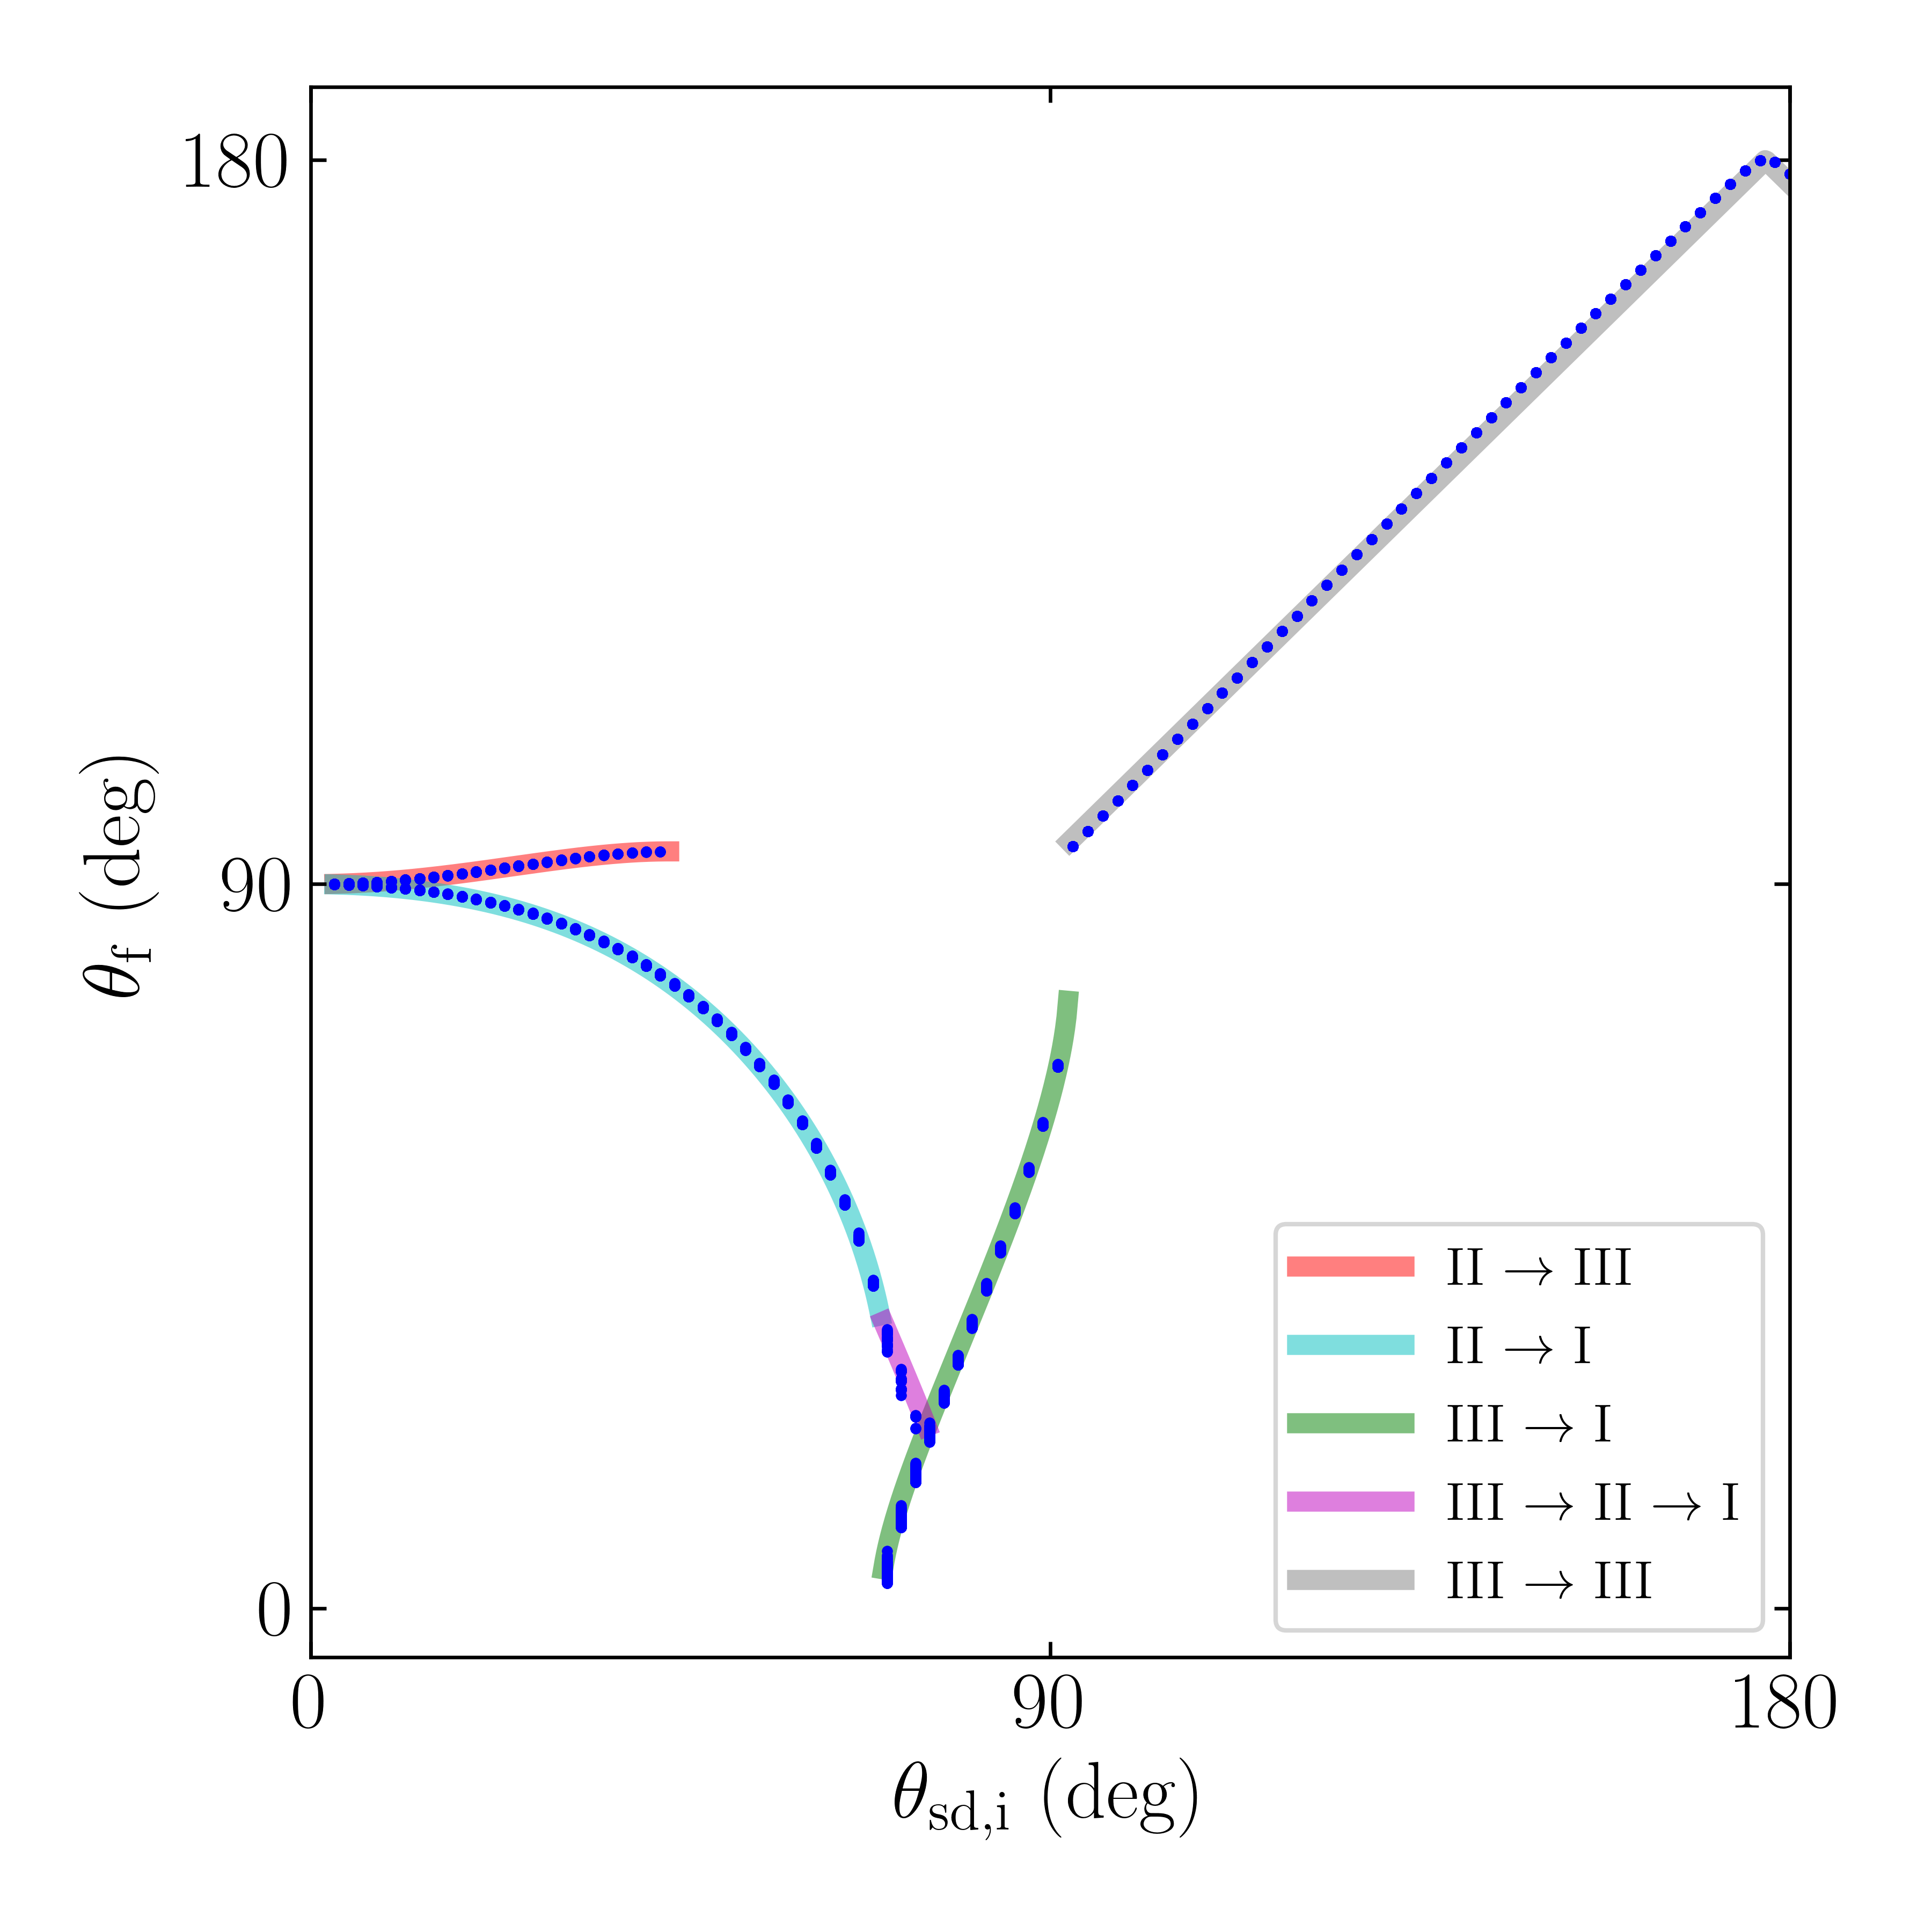
\includegraphics[width=0.5\textwidth]{../initial/2_toy2/3_ensemble_10_35.png}
    \caption{Same as the top panel of Fig.~\ref{fig:ad_ensemble} but for $I =
    10^\circ$ and with fewer annotations.}\label{fig:3_ensemble_10_35}
\end{figure}
\begin{figure}
    \centering
    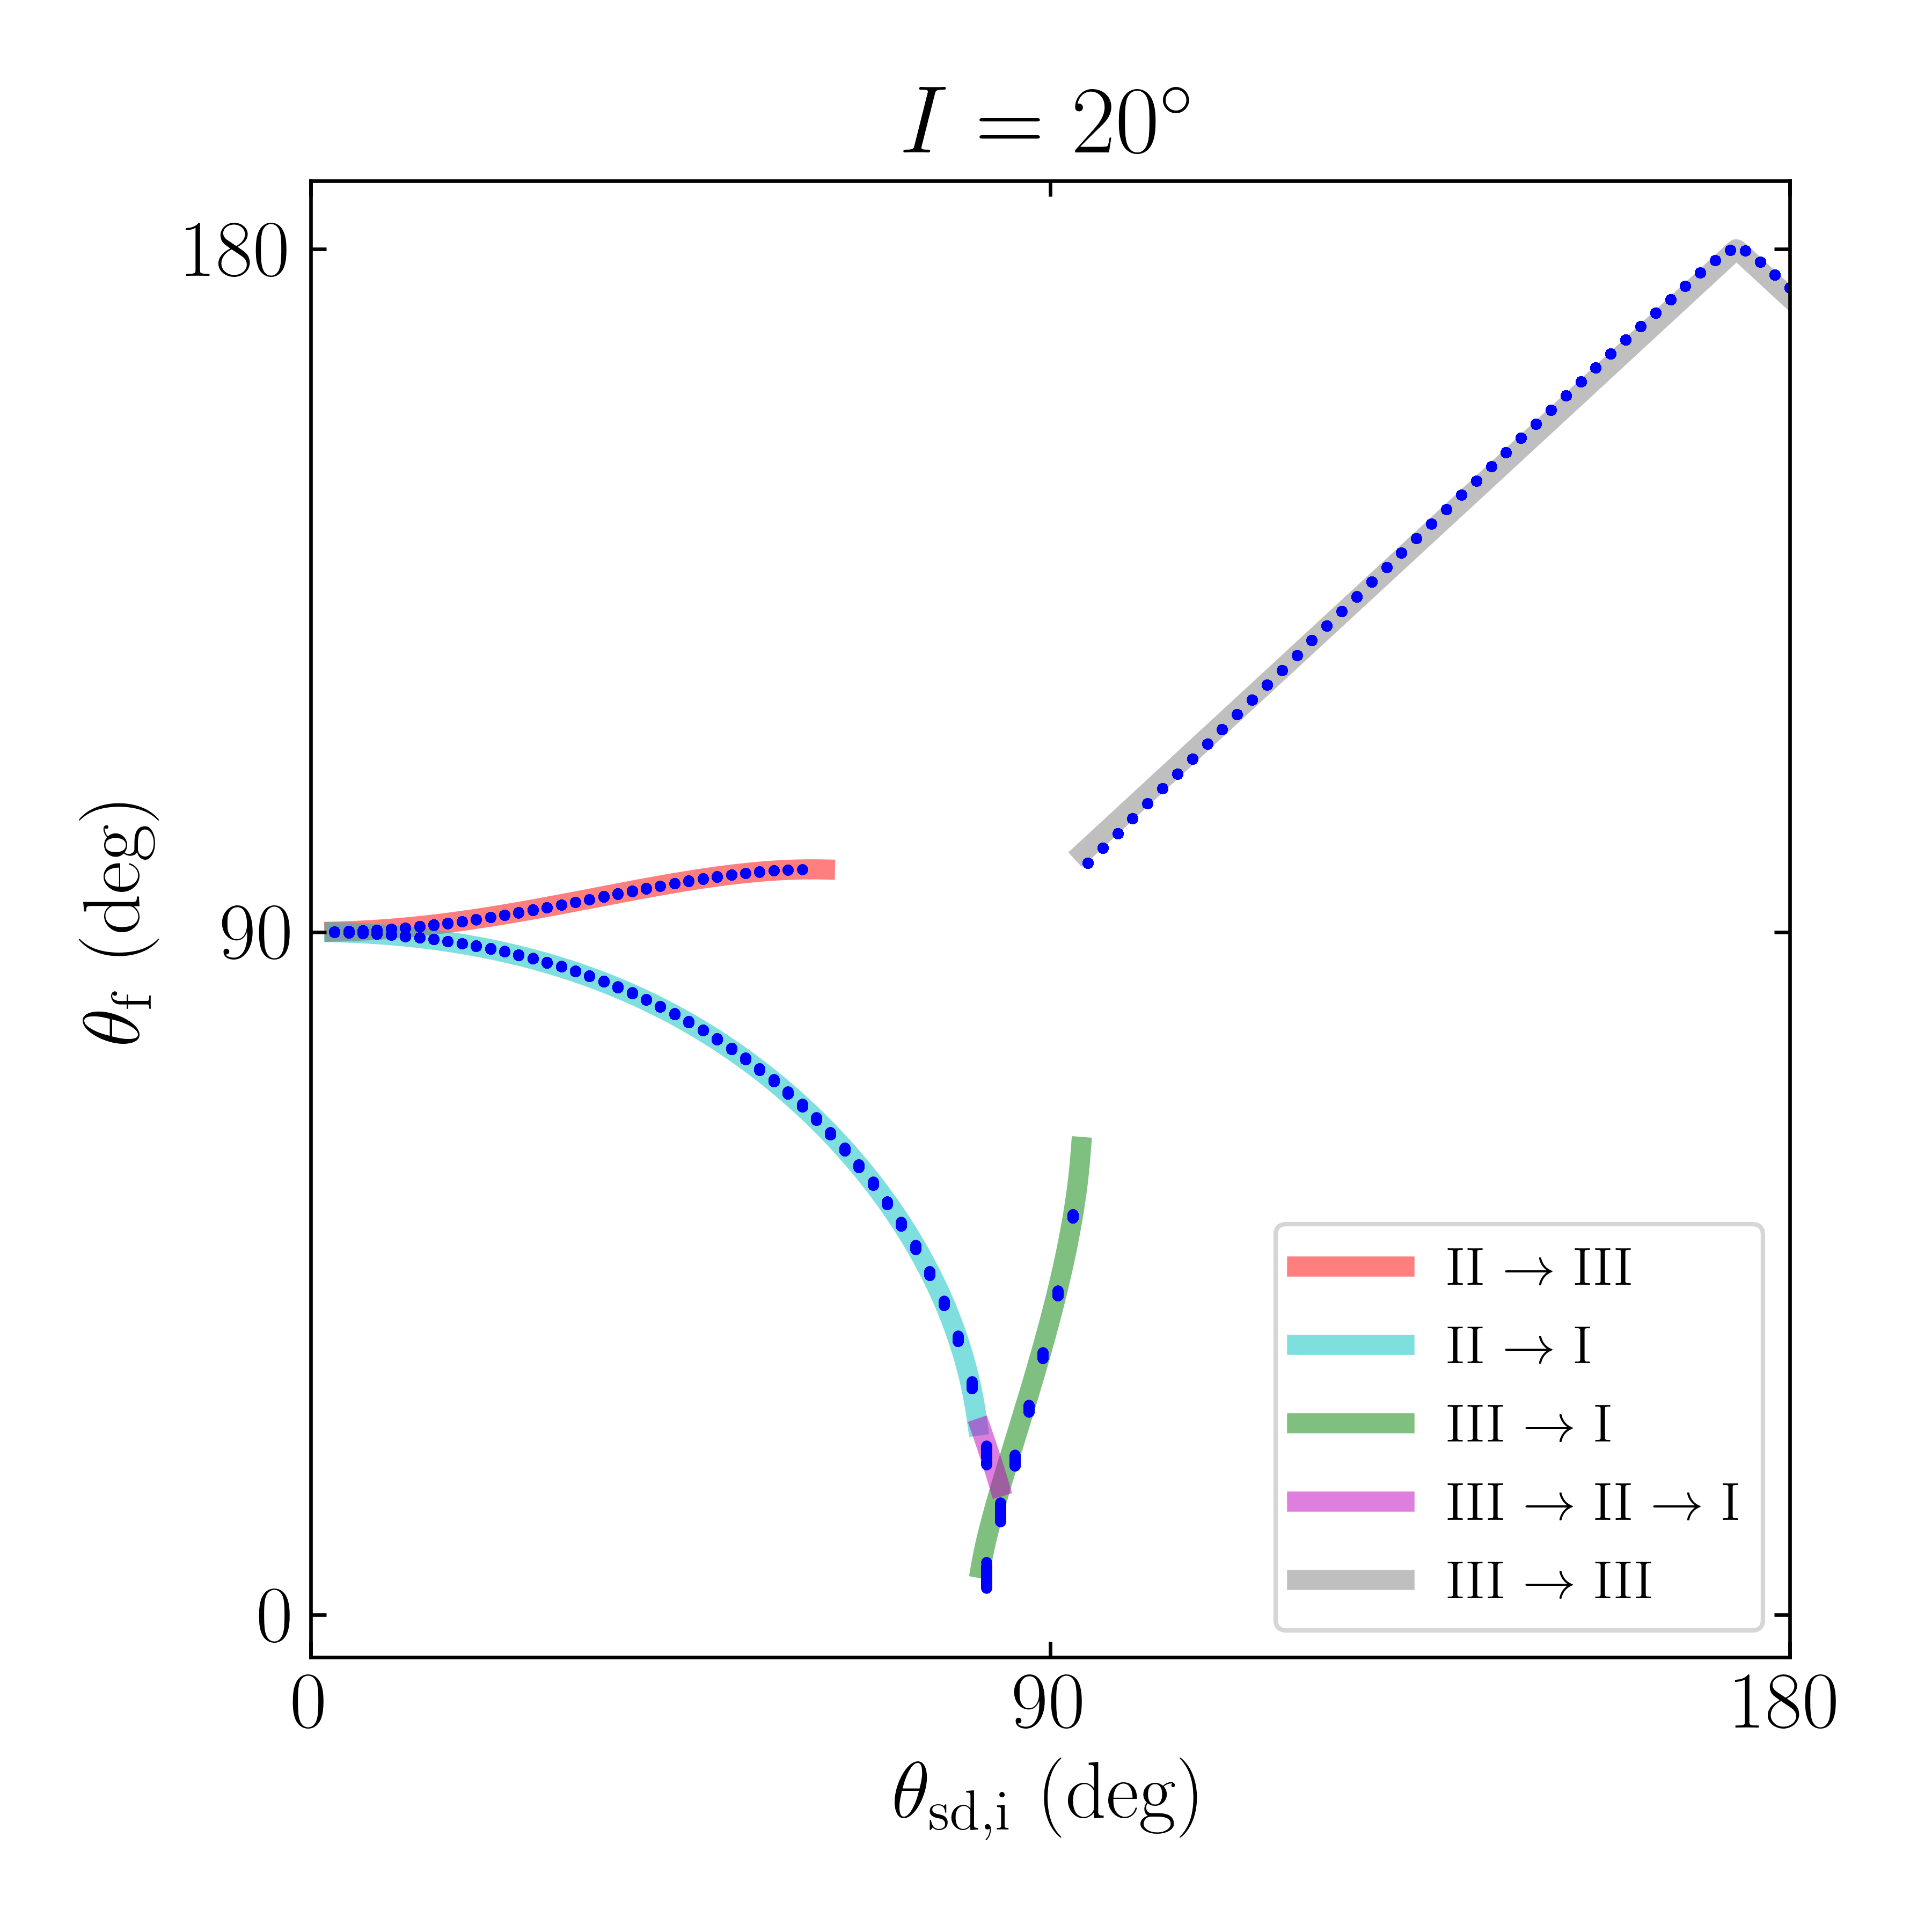
\includegraphics[width=0.5\textwidth]{../initial/2_toy2/3_ensemble_20_35.png}
    \caption{Same as the top panel of Fig.~\ref{fig:3_ensemble_10_35} but for $I
    = 20^\circ$ and with fewer annotations.}\label{fig:3_ensemble_20_35}
\end{figure}

\subsection{Analytical Theory for Adiabatic Evolution}\label{ss:zone_transitions}

The evolutionary tracks that govern the $\theta_{\rm f}$-$\theta_{\rm sd, i}$
mapping correspond to various sequences of separatrix crossings. They can be
understood using the principle of adiabatic invariance, combined with (i) how
the enclosed phase space area by the trajectory evolves across each separatrix
crossing, and (ii) the associated probabilities with each separatrix crossing.

\subsubsection{Governing Principle: Evolution of Enclosed Phase Space
Area}\label{sss:a_evo}

First, we consider how the enclosed phase space area by a trajectory evolves
over time. In the absence of separatrix encounters, the enclosed phase space
area $\oint \cos\theta \;\mathrm{d}\phi$ is an adiabatic invariant. We adopt
convention where
\begin{equation}
    A \equiv \oint \p{1 - \cos \theta}\;\mathrm{d}\phi.\label{eq:a_oint}
\end{equation}
This definition of $A$ has the advantage of (i) being continuous across
transitions from circulating to librating that cross the North pole
($\cos \theta = 1$), and (ii) being easily expressible as combinations of the
$A_{\rm i}$ of Eqs.~\eqref{se:area_ward}. The bounds of the integral are either
a libration or circulation cycle. Note that when $\eta_{\rm i} \gg 1$,
trajectories librate about $\uv{l}_{\rm d}$ with constant $\theta_{\rm sd}$,
meaning they enclose initial phase space area
\begin{equation}
    A_{\rm i} = 2\pi\p{1 - \cos \theta_{\rm sd, i}}.\label{eq:ai_qsd}
\end{equation}
Complications arise when considering finite $\eta_{\rm i}$, as trajectories near
CS2 or CS3 librate about these equilibria, rather than $\uv{l}_{\rm d}$, and
Eq.~\eqref{eq:ai_qsd} is no longer exact. In practice, Eq.~\eqref{eq:ai_qsd}
holds very well when defining $\theta_{\rm sd, i}$ as the angular distance to
CS2; an exception is discussed in Section~\ref{sss:evol_traj}.

Beginning at the last separatrix crossing, the final enclosed phase space area
$A_{\rm f}$ will be conserved for all time. As $\eta \to 0$, trajectories circulate at
constant obliquity $\theta_{\rm f}$, related to $A_{\rm f}$ by
\begin{equation}
    2\pi\p{1 - \cos \theta_{\rm f}} = A_{\rm f}. \label{eq:qfaf}
\end{equation}

$A$ is not conserved when the trajectory encounters the separatrix. Howover, its
change is easily understood \citep{henrard1982}. In essence, when the trajectory
crosses the separatrix, it continues to evolve adjacent to the separatrix. So if
a separatrix crossing results in a zone I trajectory, the resultant $A$ can be
approximated by integrating Eq.~\eqref{eq:a_oint} along the upper leg of the
separatrix. Pictorally, this can be seen in the bottom plots of
Fig.~\ref{fig:ad_21}.

\subsubsection{Governing Principles: Probabilistic Separatrix Crossing}

When a trajectory experiences separatrix crossing, it transitions into nearby
zones probabilistically. This process is well understood by
\citealp{henrard1982,henrard1987}. Their results may be simply summarized as
follows: if a zone $i$ is shrinking while adjacent zones $j, k$ are expanding
such that the sum of their areas is constant, the probability of transition from
zone $i$ to zone $j$ is given
\begin{align}
    \Pr\p{i \to j} = -\frac{\pd{A_{\rm j}}{t}}{ \pd{A_{\rm i}}{t}}
        = -\frac{\pd{A_{\rm j}}{\eta}}{ \pd{A_{\rm i}}{\eta}},\\
    \Pr\p{i \to k}
        = -\frac{\pd{A_{\rm k}}{\eta}}{ \pd{A_{\rm i}}{\eta}}.\label{eq:henrard_hop}
\end{align}
Note that $\Pr \p{i \to j} + \Pr\p{i \to k} = 1$. This can be used directly in
conjunction with Eqs.~\eqref{se:area_ward} to understand for what initial
conditions each track can be observed and with what probabilities.

As a particular example, consider a system in zone II in panel (d) of
Fig.~\ref{fig:eq_1contours}. As $\eta decreases, zone II$ will shrink while
zones I and III will expand until the trajectory. Suppose the trajectory
exits zone II at some $\eta_\star$, then the probability of a II $\to$ I
transition is $\Pr\p{\rm II \to I} = -\frac{\dot{A}_{\rm I}}{\dot{A}_{\rm II}}$,
while a II $\to$ III transition occurs with probability $\Pr\p{\rm II \to III} =
-\frac{\dot{A}_{\rm III}}{\dot{A}_{\rm II}}$.

\subsubsection{Evolutionary Trajectories}\label{sss:evol_traj}

Returning to the evolution of $\uv{s}$, we can classify trajectories by the
separatrix encounters experienced. Initially, in the $\eta > \eta_{\rm c}$ regime,
only zones II and III exist. Conversely, at the end of the simulation when $\eta
\to 0$, only zones I and III exist. Most simply, one might expect four sequences
of transitions between zones (we call these dynamical ``tracks'') to manifest:
from one of $\z{I, III}$ to one of $\z{II, III}$, where III $\to$ III is a
trivial case (no separatrix encounter). In addition to these four tracks, a
fifth track III $\to$ II $\to$ I is observed. Below, we will describe the
evolution of $A$ throughout each of the five tracks, as well as determine the
initial conditions and probabilities associated with each track:
\begin{enumerate}
    \item II $\to$ I --- An example trajectory following this track is depicted
        in Fig.~\ref{fig:ad_21}. $\uv{s}$ starts librating about CS2 in zone II,
        enclosing some initial phase space area $A_{\rm i}$. The trajectory is
        able to librate without separatrix encounter until $A_{\rm
        II}(\eta_\star) = A_{\rm i}$. As the trajectory transitions to a
        circulating trajectory in zone I immediately bordering the separatrix,
        it will encompass $-A_{\rm I}(\eta_\star)$ phase space area. The final
        $\theta_{\rm f}$ is then given by Eq.~\eqref{eq:qfaf}. An analytical
        approximation to $\theta_{\rm f}$ is derived in
        Appendix~\ref{s:ad_approx} and is
        \begin{equation}
            \cos \theta_{\rm f, II \Rightarrow I} \approx
                \p{\frac{\pi \theta_{\rm sp, i}^2}{16}}^2 \cot I
                    + \frac{\theta_{\rm sp, i}^2}{4}.\label{eq:qf_21_approx}
        \end{equation}

        This transition can only occur when the initial condition begins in zone
        II, requiring $A_{\rm i} < A_{\rm II}(\eta_{\rm c})$. Note $A_{\rm II}(\eta_{\rm c})$ is
        given in closed form in \citet{ward2004I} but appears to be incorrect.
        Then, at some known $\eta_\star$ satisfying $A_{\rm II}(\eta_\star) =
        A_{\rm i}$, the trajectory is ejected from the separatrix following
        Eq.~\eqref{eq:henrard_hop}. Note that since $\pd{A_{\rm i}}{\eta} < 0$
        everywhere, while $\pd{A_{\rm II}}{\eta} > 0$ at all possible
        $\eta_\star$ for an initial condition starting in zone II, this track
        always has nonzero probability.

    \item II $\to$ III --- An example trajectory following this track is
        depicted in Fig.~\ref{fig:ad_23}. The only difference from the previous
        track is that, upon separatrix encounter, the trajectory follows the
        circulating trajectory in zone III bordering the separatrix, upon
        which it will encompass $A_{\rm f} = A_{\rm I}(\eta_\star) + A_{\rm
        II}(\eta_\star)$. The final obliquity is still given by
        Eq.~\eqref{eq:qfaf}, and the analytical approximation derived in
        Appendix~\ref{s:ad_approx} is
        \begin{equation}
            \cos \theta_{\rm f, II \Rightarrow III} \approx
                \p{\frac{\pi \theta_{\rm sp, i}^2}{16}}^2 \cot I
                    - \frac{\theta_{\rm sp, i}^2}{4}.\label{eq:qf_23_approx}
        \end{equation}

        Again, this track can only occur when $A_{\rm i} < A_{\rm II}(\eta_{\rm c})$, but a
        further constraint arises when we consider the transition probability
        given by Eq.~\eqref{eq:henrard_hop}. Upon examination of
        Fig.~\ref{fig:eq_areas}, it is clear that $\pd{A_{\rm III}}{\eta} > 0$ for
        many $\eta$. Call
        \begin{equation}
            \eta_{\min, III} \equiv \argmin A_{\rm III}(\eta)
                \label{eq:eta_minIII},
        \end{equation}
        which is labeled in Fig.~\ref{fig:eq_areas}, then if $\eta_\star >
        \eta_{\rm \min, III}$ then $\Pr_{\rm II \to III} < 0$. This is
        understood as a forbidden transition, and so II $\to$ III is only a
        permitted dynamical track if $\eta_\star <, \eta_{\rm \min, III}$.

    \item III $\to$ I --- This track is depicted in Fig.~\ref{fig:ad_31}.
        The trajectory encounters the separatrix when $A_{\rm I}(\eta_\star) +
        A_{\rm II}(\eta_\star) = A_{\rm i}$, upon which it transitions to a zone
        I trajectory enclosing $A_{\rm f} = -A_{\rm I}$. Then, as always, the
        final obliquity is given by Eq.~\eqref{eq:qfaf}.

        This track can only occur if $A_{\rm i} > A_{\rm II}(\eta_{\rm c})$, but is also
        constrained by requiring its $A_{\rm i}$ is sufficiently small it will
        encounter the separatrix (if it is too large, it will never encounter
        the separatrix, which is a III $\to$ III transition). This is written
        $A_{\rm i} < \max A_{\rm I} + A_{\rm II} = 4\pi - \min A_{\rm III}$.

        Note that since $\pd{A_{\rm I}}{\eta} < 0$ always while $\pd{A_{\rm
        III}}{\eta} > 0$ for all accessible $\eta_{\star}$, this track is always
        permitted.

    \item III $\to$ II $\to$ I --- This track is depicted in
        Fig.~\ref{fig:ad_321}. The first separatrix encounter occurs at $\eta_1$
        when $A_{\rm I}(\eta_1) + A_{\rm II}(\eta_1) = A_{\rm i}$, upon which
        the trajectory moves into zone II enclosing intermediate phase space
        area $A_{\rm m} = A_{\rm II}(\eta_1)$. Examining
        Fig.~\ref{fig:eq_areas}, there exist values $A$ for which $A_{\rm
        II}(\eta) = A$ has multiple solutions, and $\eta_1 > \eta_{\rm II,
        \max}$ as labeled. These are the only values for which the III $\to$ II
        $\to$ I transition is permitted. Thus, as $\eta$ continues to decrease,
        a second $\eta_2$ value exists for which $A_{\rm m} = A_{\rm
        II}(\eta_2)$, upon which the trajectory is ejected to zone I and $A_f =
        -A_{\rm I}(\eta_2)$. The final obliquity again then obeys
        Eq.~\eqref{eq:qfaf}.

        Similar to the III $\to$ I track, the III $\to$ II $\to$ I track can
        only occur over the same $A_{\rm II}(\eta_{\rm c}) < A_{\rm i} < \max
        A_{\rm I} + A_{\rm II}$ interval. The probability of encountering this
        track is set by the initial III $\to$ II transition. It bears noting
        that this probability is only nonnegative for a very small fraction of
        $A_{\rm i}$ values, since it requires $\pd{A_{\rm II}}{\eta}$ and
        $\pd{A_{\rm III}}{\eta}$ to have different signs; this occurs only if
        $A_{\rm II}\p{\eta_{\rm c}} < A_{\rm i} < A_{\rm II, \max}$. Outside of
        these bounds, $\Pr_{\rm III \to II} < 0$ which is interpreted again as a
        forbidden transition.

        Then, once a III $\to$ II transition occurs, the second II $\to$ I
        transition occurs for some $\eta_2$ satisfying $A_{\rm II}(\eta_2) =
        A_{\rm II}(\eta_1), \eta_2 < \eta_1$. Graphical inspection shows that
        $\pd{A_{\rm II}}{\eta}$ has the same sign as $\pd{A_{\rm III}}{\eta}$
        over all possible values, so the second II $\to$ I transition is
        guaranteed, completing the III $\to$ II $\to$ I track.

    \item III $\to$ III --- This track depicts the trivial case where no
        separatrix encounter ever occurs, and $A$ is constant throughout the
        evolution. This constraint equates to $A_{\rm i} > \max A_{\rm I} + A_{\rm
        II}$, whereupon no separatrix encounter occurs at all, and $A_{\rm f} =
        A_{\rm i}$,
        which for $\eta_{\rm i} \to \infty, \eta_{\rm f} \to 0$ results in $\theta =
        \theta_{\rm sd, i}$.

        Note that a small deviation from $\theta = \theta_{\rm sd, i}$ occurs
        because we use finite $\eta_{\rm i}$, as hinted at in Section~\ref{sss:a_evo}.
        This is because for $\theta_{\rm sd, i} \gtrsim \pi/2$, trajectories are
        better described as librating about CS3. Nevertheless, we can still
        approximate $A_{\rm i}$ to good accuracy as the solid angle enclosed by
        libration about CS3 with polar angle $2\pi + \theta_3 - \theta_2 -
        \theta_{\rm sd, i}$. This recovers the correct transfer function
        $\theta_{\rm f}\p{\theta_{\rm sd, i}}$ for the III $\to$ III regime, as
        can be seen visibly in Fig.~\ref{fig:3_ensemble_20_35}.
\end{enumerate}
In summary, the five regimes of track possibilities in increasing order of
$A_{\rm i}$
are:
\begin{enumerate}
    \item $A_{\rm i} \in \s{0, A_{\rm II}\p{\eta_{\rm \min, III}}}$ --- II $\to$
        III and II $\to$ I both possible.

    \item $A_{\rm i} \in \s{A_{\rm II}\p{\eta_{\rm \min, III}}, A_{\rm
        II}(\eta_{\rm c})}$ --- II $\to$ I only.

    \item $A_{\rm i} \in \s{A_{\rm II}(\eta_{\rm c}), A_{\rm II, \max}}$ ---
        III $\to$ I and III $\to$ II $\to$ I both possible.

    \item $A_{\rm i} \in \s{A_{\rm II, \max}, \max A_{\rm I} + A_{\rm II}}$ ---
        III $\to$ I only.

    \item $A_{\rm i} > \max A_{\rm I} + A_{\rm II}$ --- III $\to$ III only.
\end{enumerate}
The corresponding ranges for for $\theta_{\rm sd,i}$ can be computed via
Eq.~\eqref{eq:ai_qsd}. The boundaries between these ranges are overplotted in
Fig.~\ref{fig:ad_ensemble}, where they can be seen to agree well with numerical
results.
\begin{figure}
    \centering
    \begin{subfigure}{\columnwidth}
        \centering
        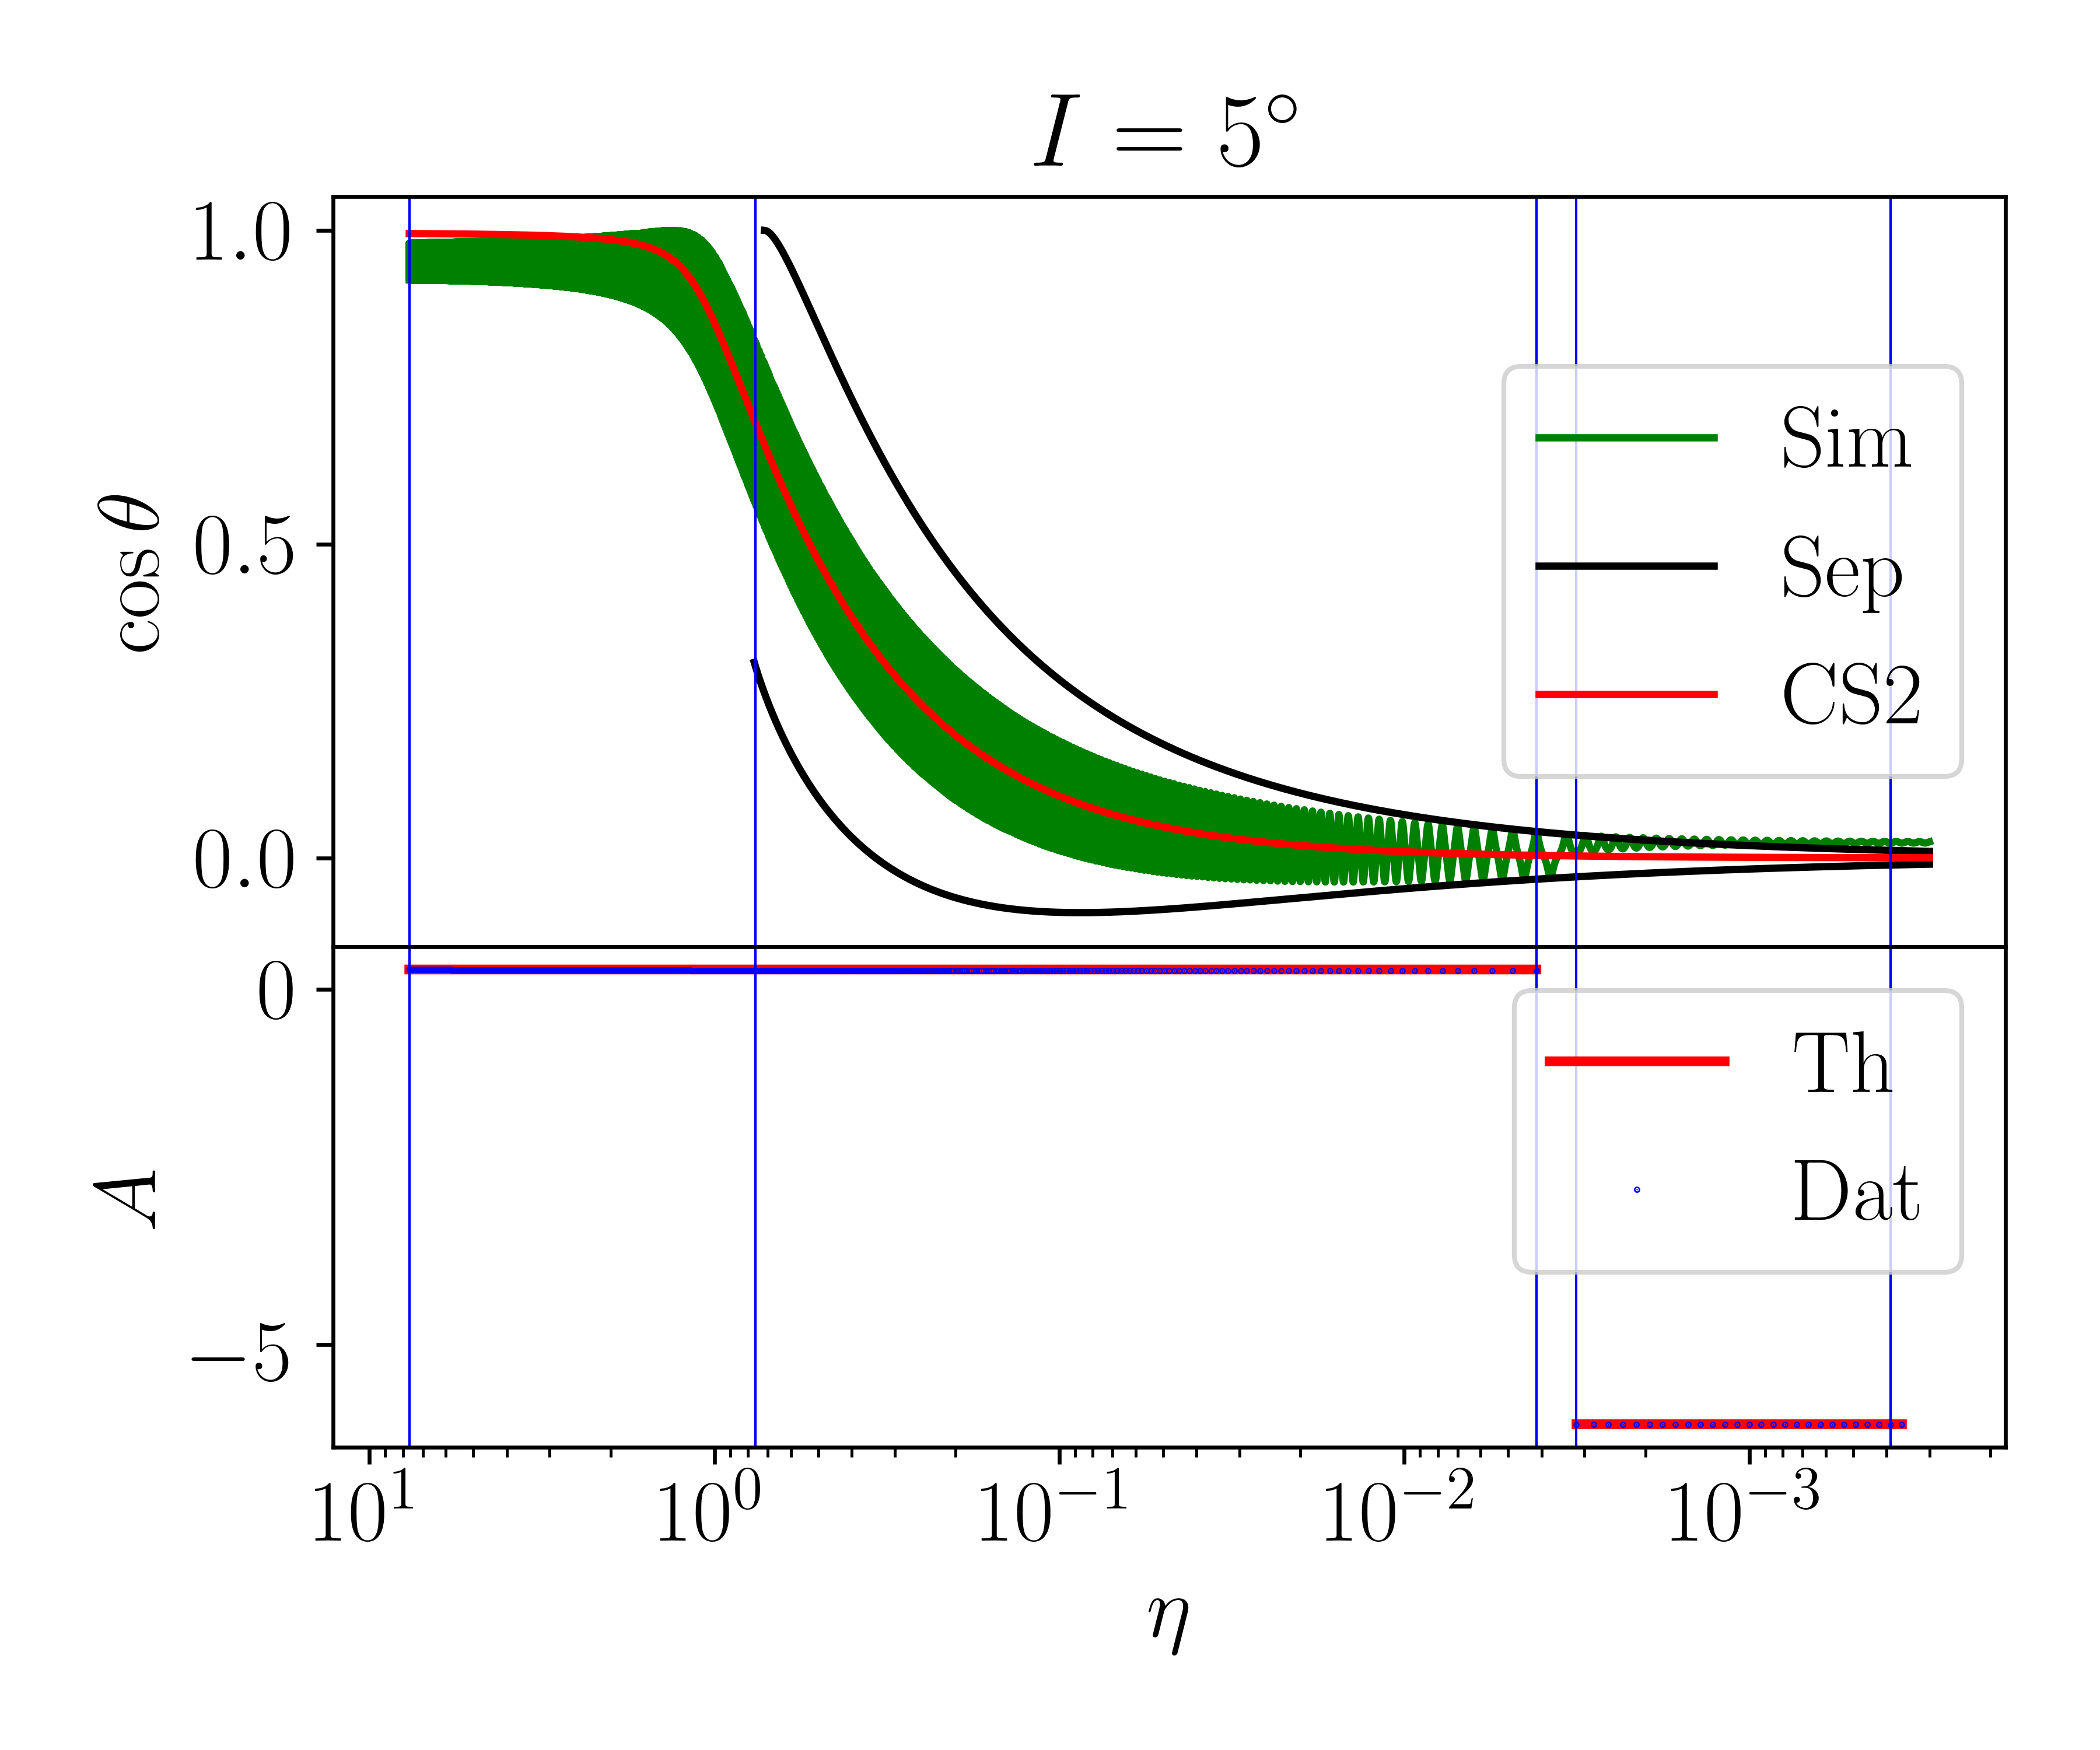
\includegraphics[width=0.5\textwidth]{../initial/2_toy2/3testo21.png}
    \end{subfigure}
    \begin{subfigure}{\columnwidth}
        \centering
        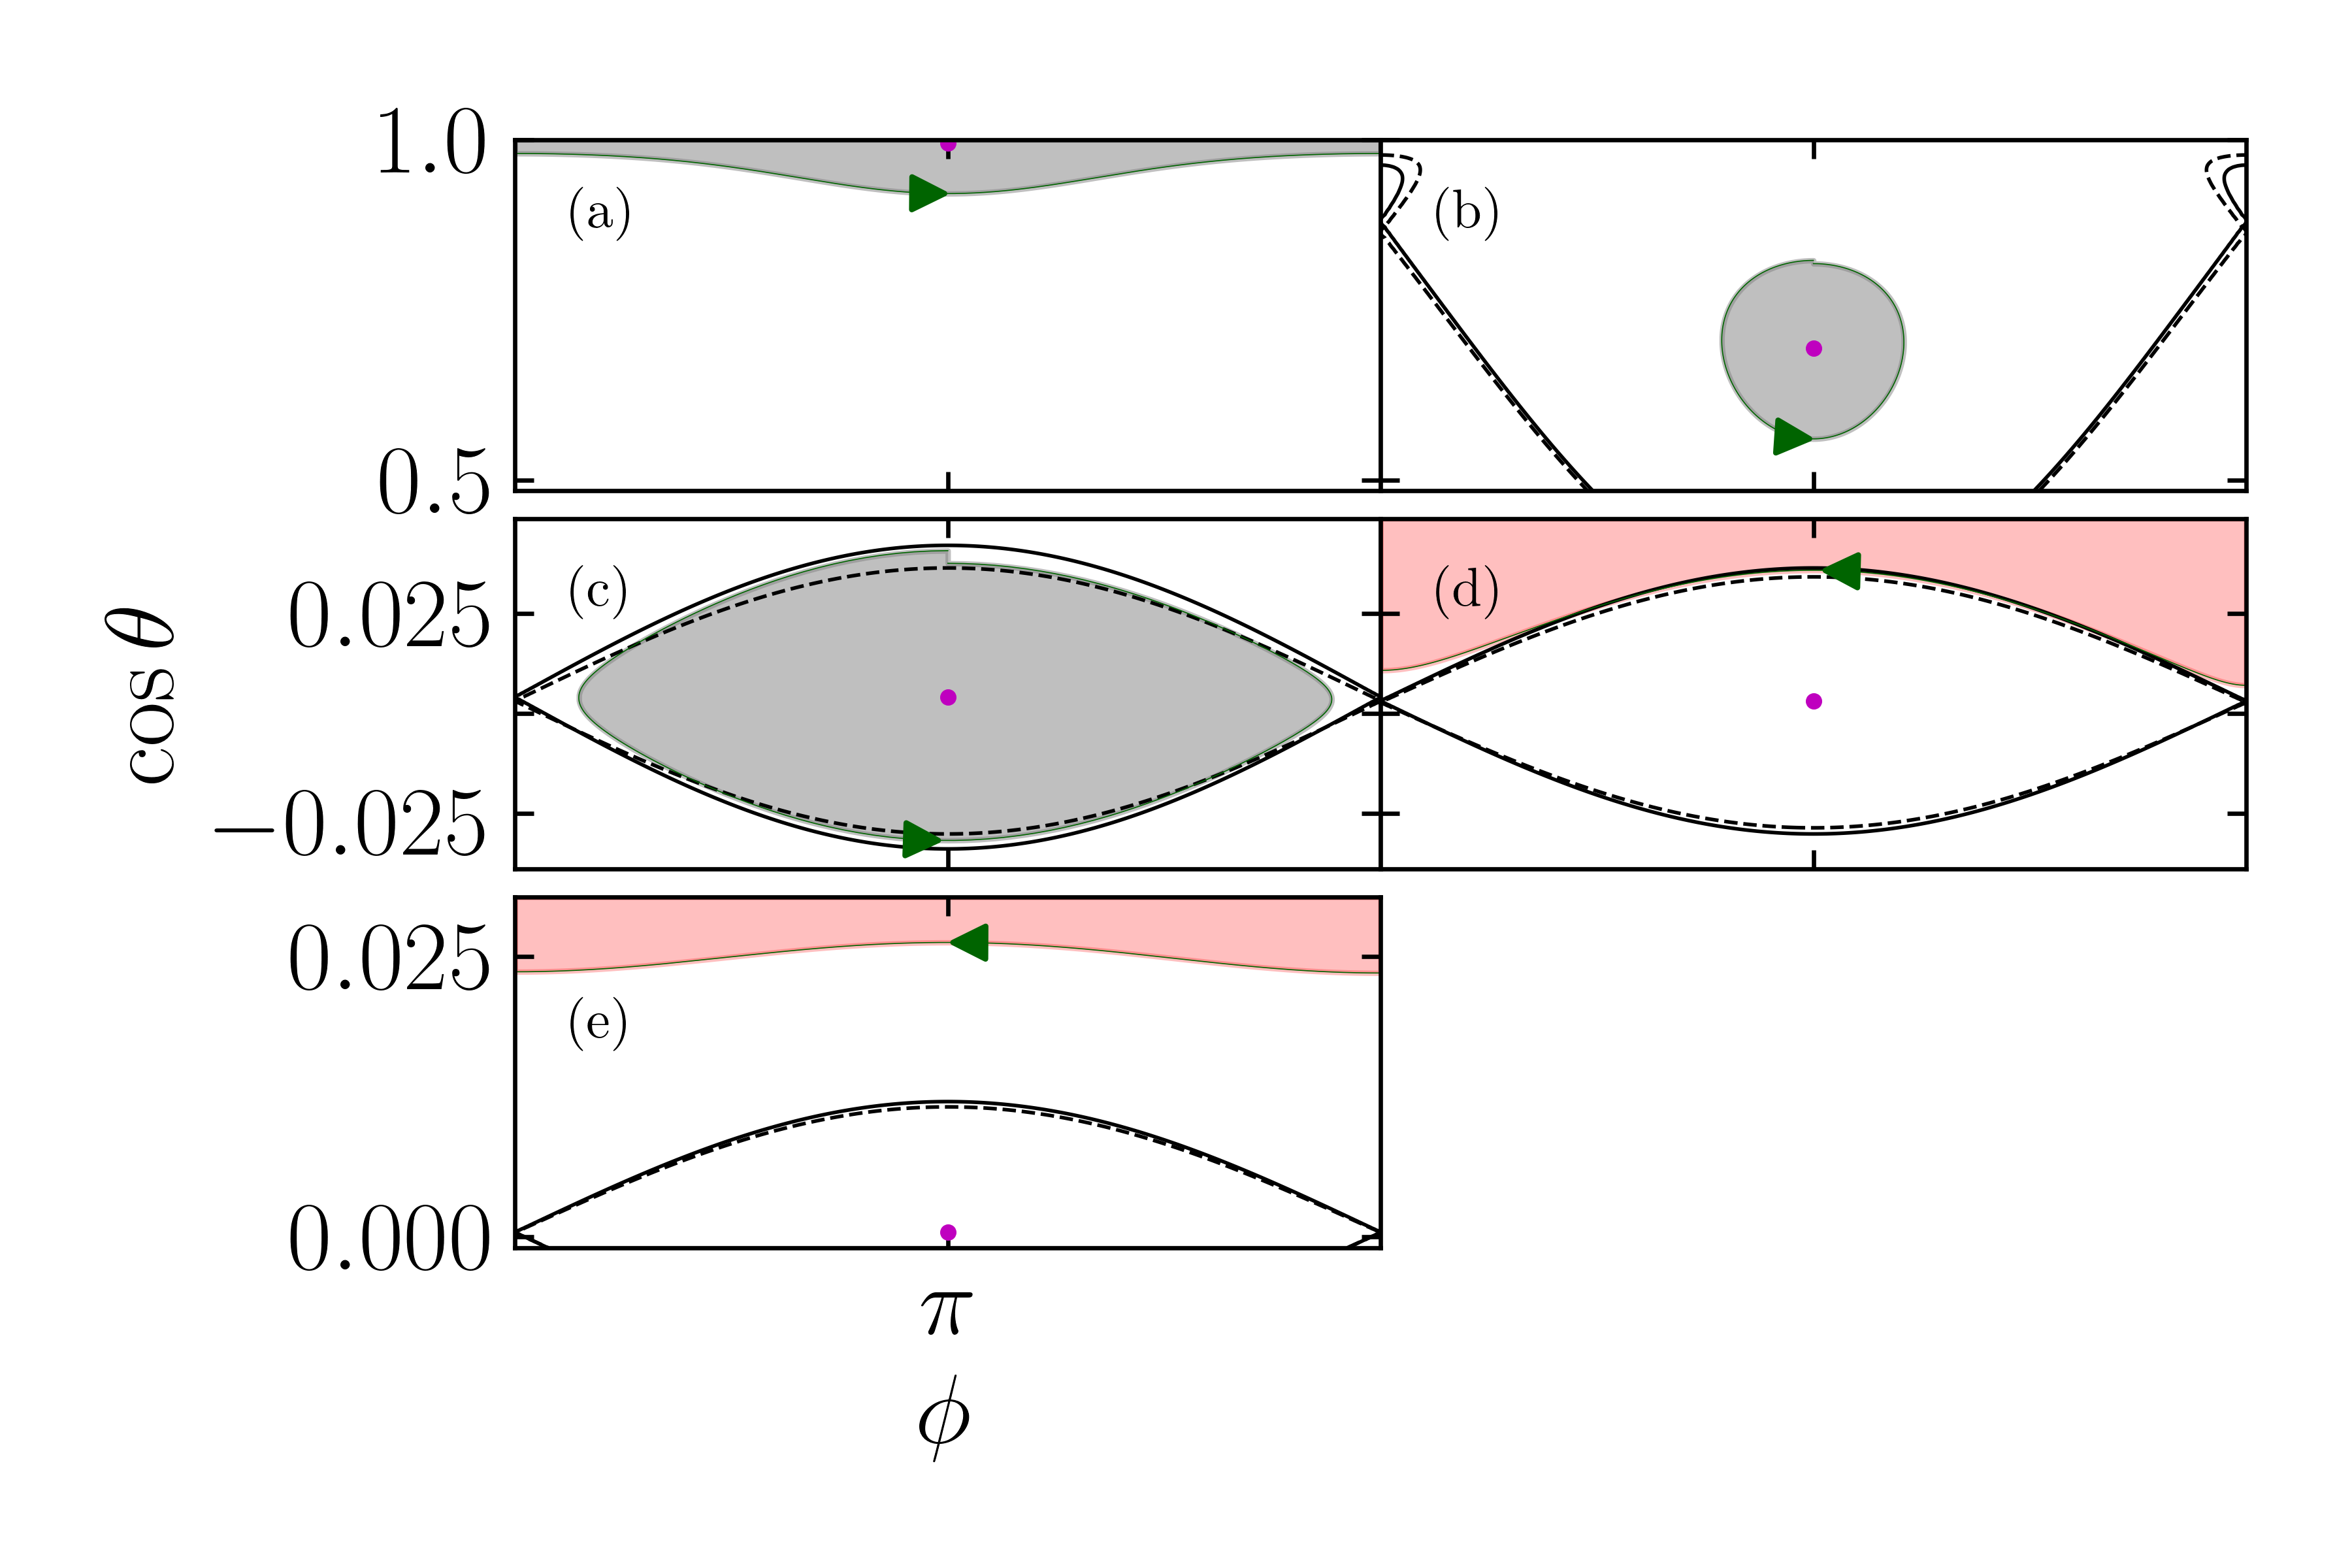
\includegraphics[width=0.5\textwidth]{../initial/2_toy2/3testo21_subplots.png}
    \end{subfigure}
    \caption{Fiducial simulation following the $A_{\rm II} \to A_{\rm I}$
    transition. An initial $\theta_{\rm sd, i} = 0.3\;\mathrm{rad} \approx
    17.2^\circ$ was used, as well as $\epsilon = 3 \times 10^{-4}$. Top plot
    upper panel: plot of $\cos \theta(t)$ (green) in an example simulation.
    Overlaid are the locations of Cassini State 2 (red), and upper and lower
    bounds on the separatrix (black). Note that the trajectory successfully
    tracks CS2 to an obliquity $\theta \approx 90^\circ$. Light vertical blue
    lines denote times portrayed in bottom plot. Top plot lower panel: plot of
    the enclosed separatrix area obtained by integrating the simulated
    trajectory (blue dots) and adiabatic theory (red line). Even though the
    enclosed area jumps at separatrix crossing, the resultant $A$ is still
    accurately predicted. Lower plot: snapshots in the $\p{\cos \theta, \phi}$
    space of the simulation trajectories for the vertical blue lines in the top
    plots. These times correspond to the start of the simulation, the appearance
    of the separatrix, two panels depicting the separatrix crossing process, and
    a final snapshot at $\eta = 10^{-3.5}$. The green line denotes a full
    circulation or libration cycle at the selected time, including an arrow for
    directionality. The separatrix at the start/end of the portrayed cycle are
    shown in solid/dashed black lines respectively. Also labeled is CS2 at the
    start of the cycle (red). Finally, the enclosed phase space area is shaded
    in grey ($A > 0$) and red ($A < 0$).}\label{fig:ad_21}
\end{figure}
\begin{figure}
    \centering
    \begin{subfigure}{\columnwidth}
        \centering
        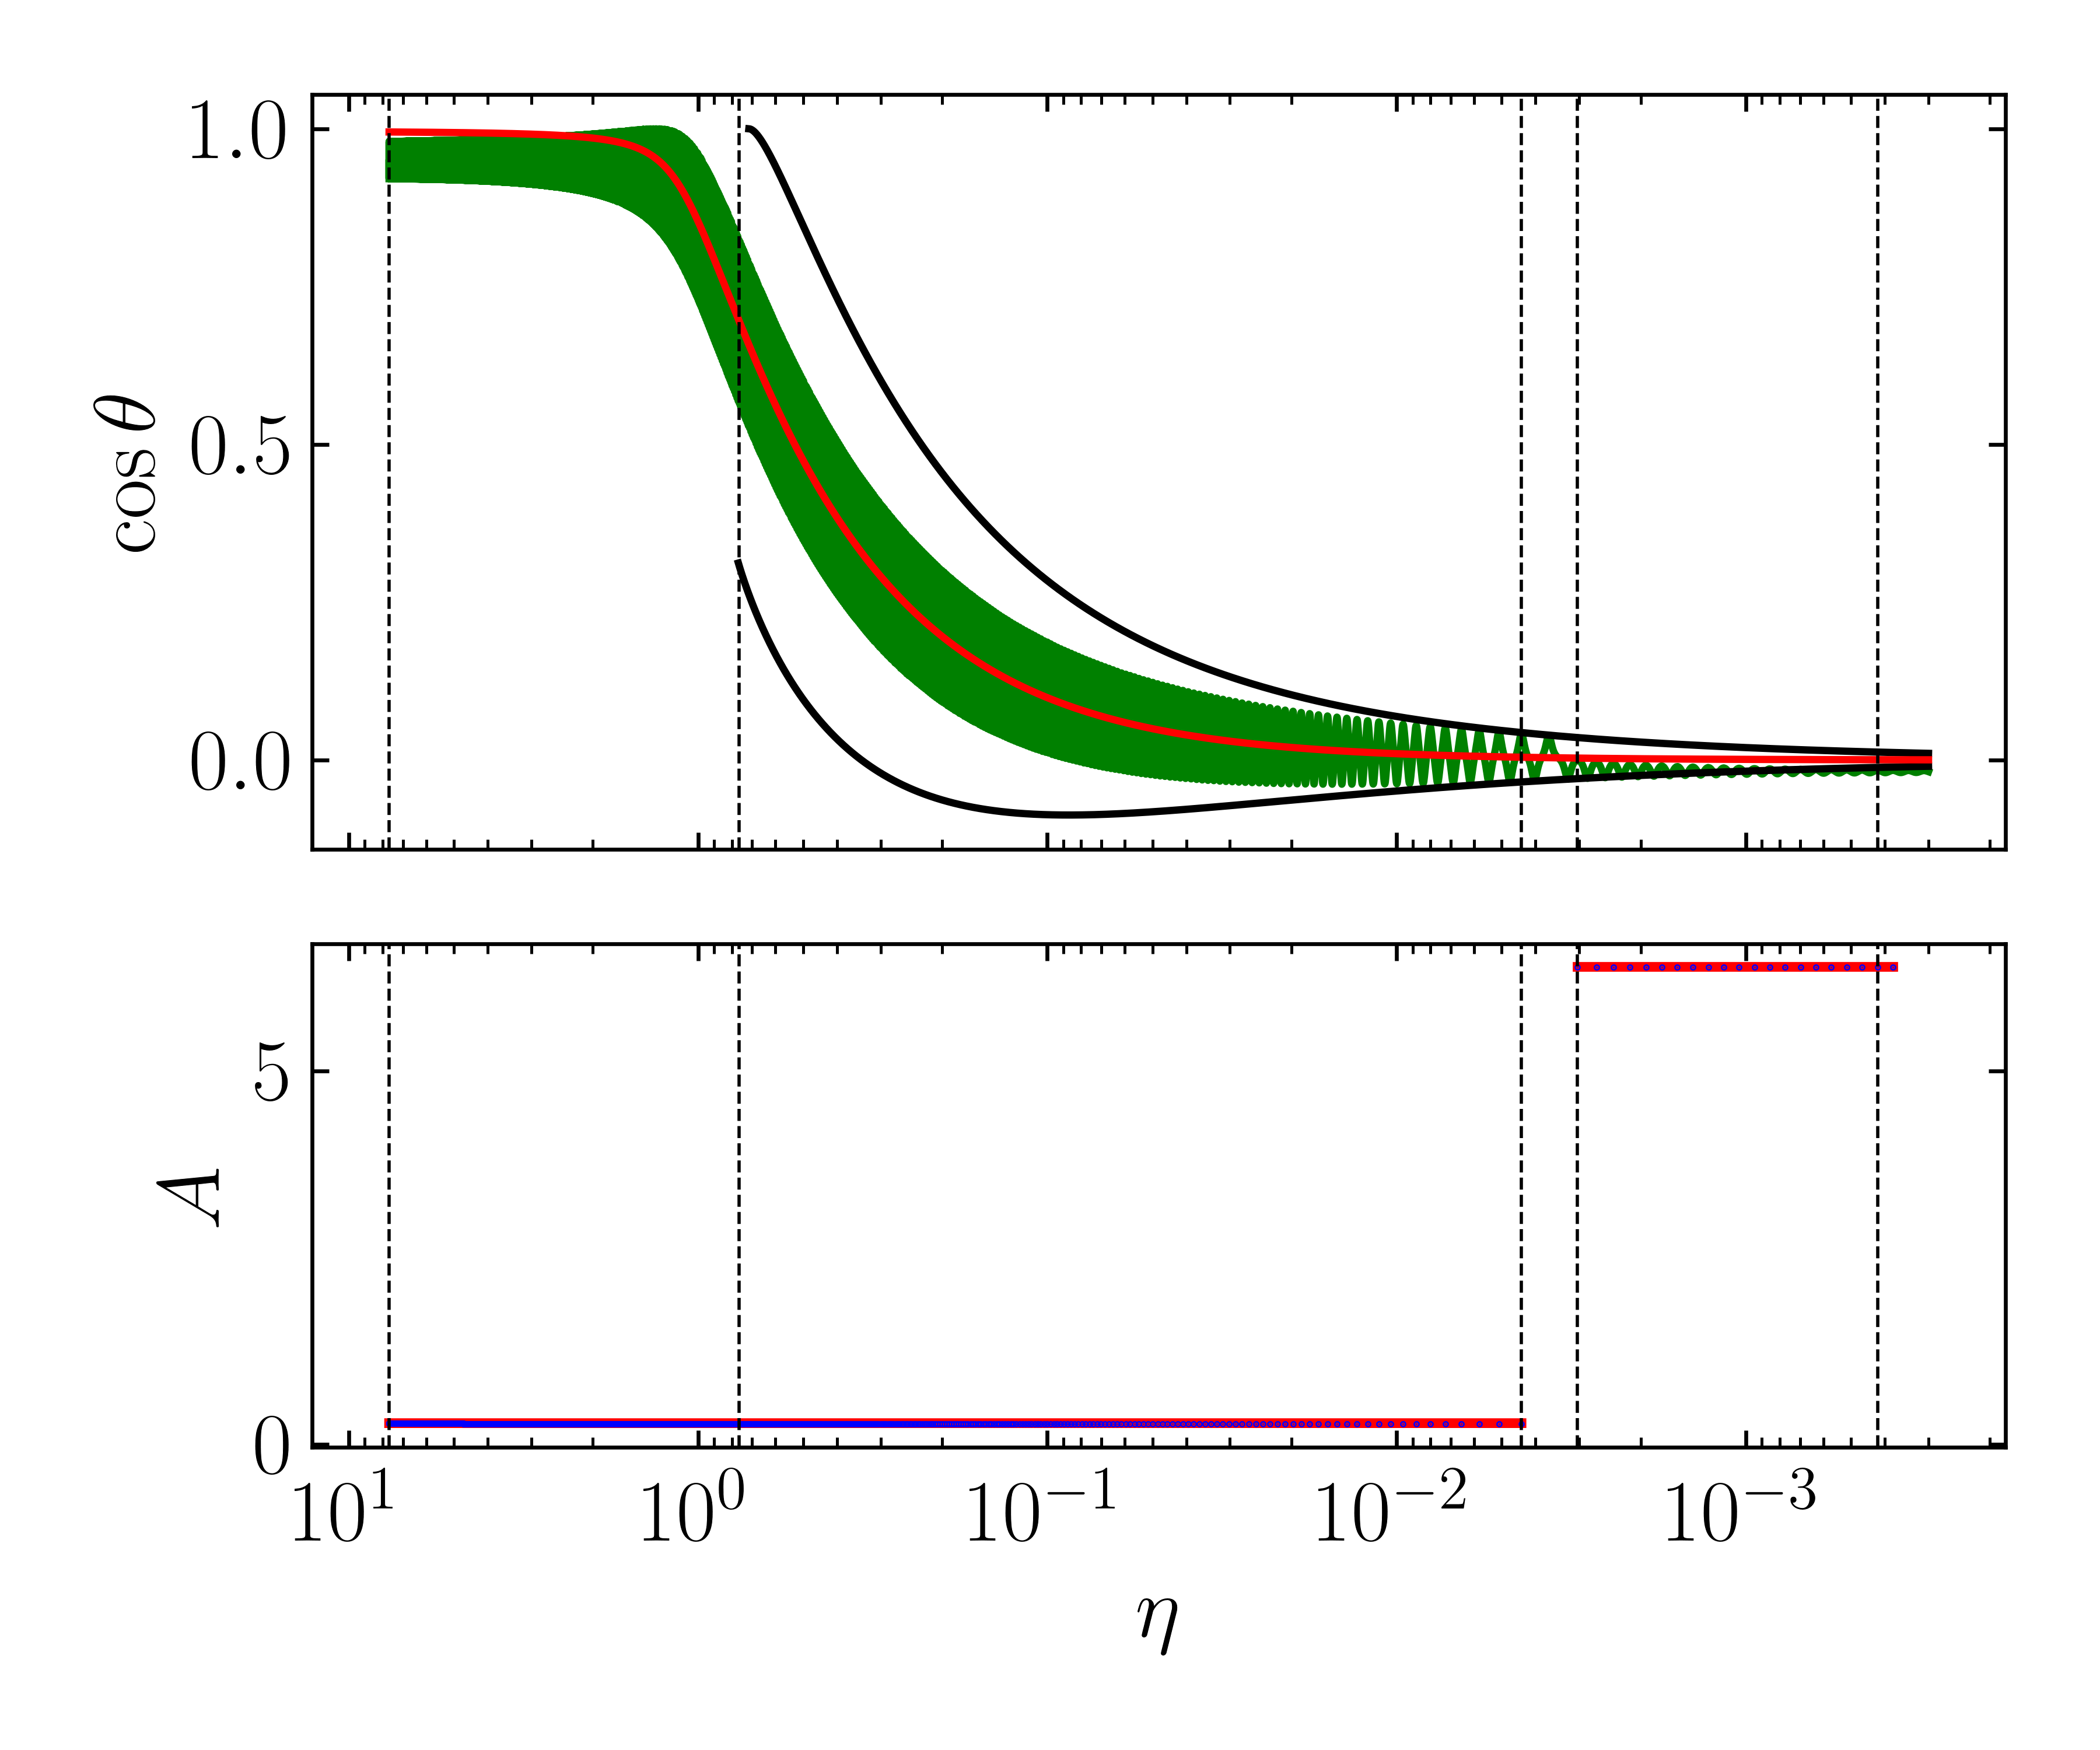
\includegraphics[width=0.5\textwidth]{../initial/2_toy2/3testo23.png}
    \end{subfigure}
    \begin{subfigure}{\columnwidth}
        \centering
        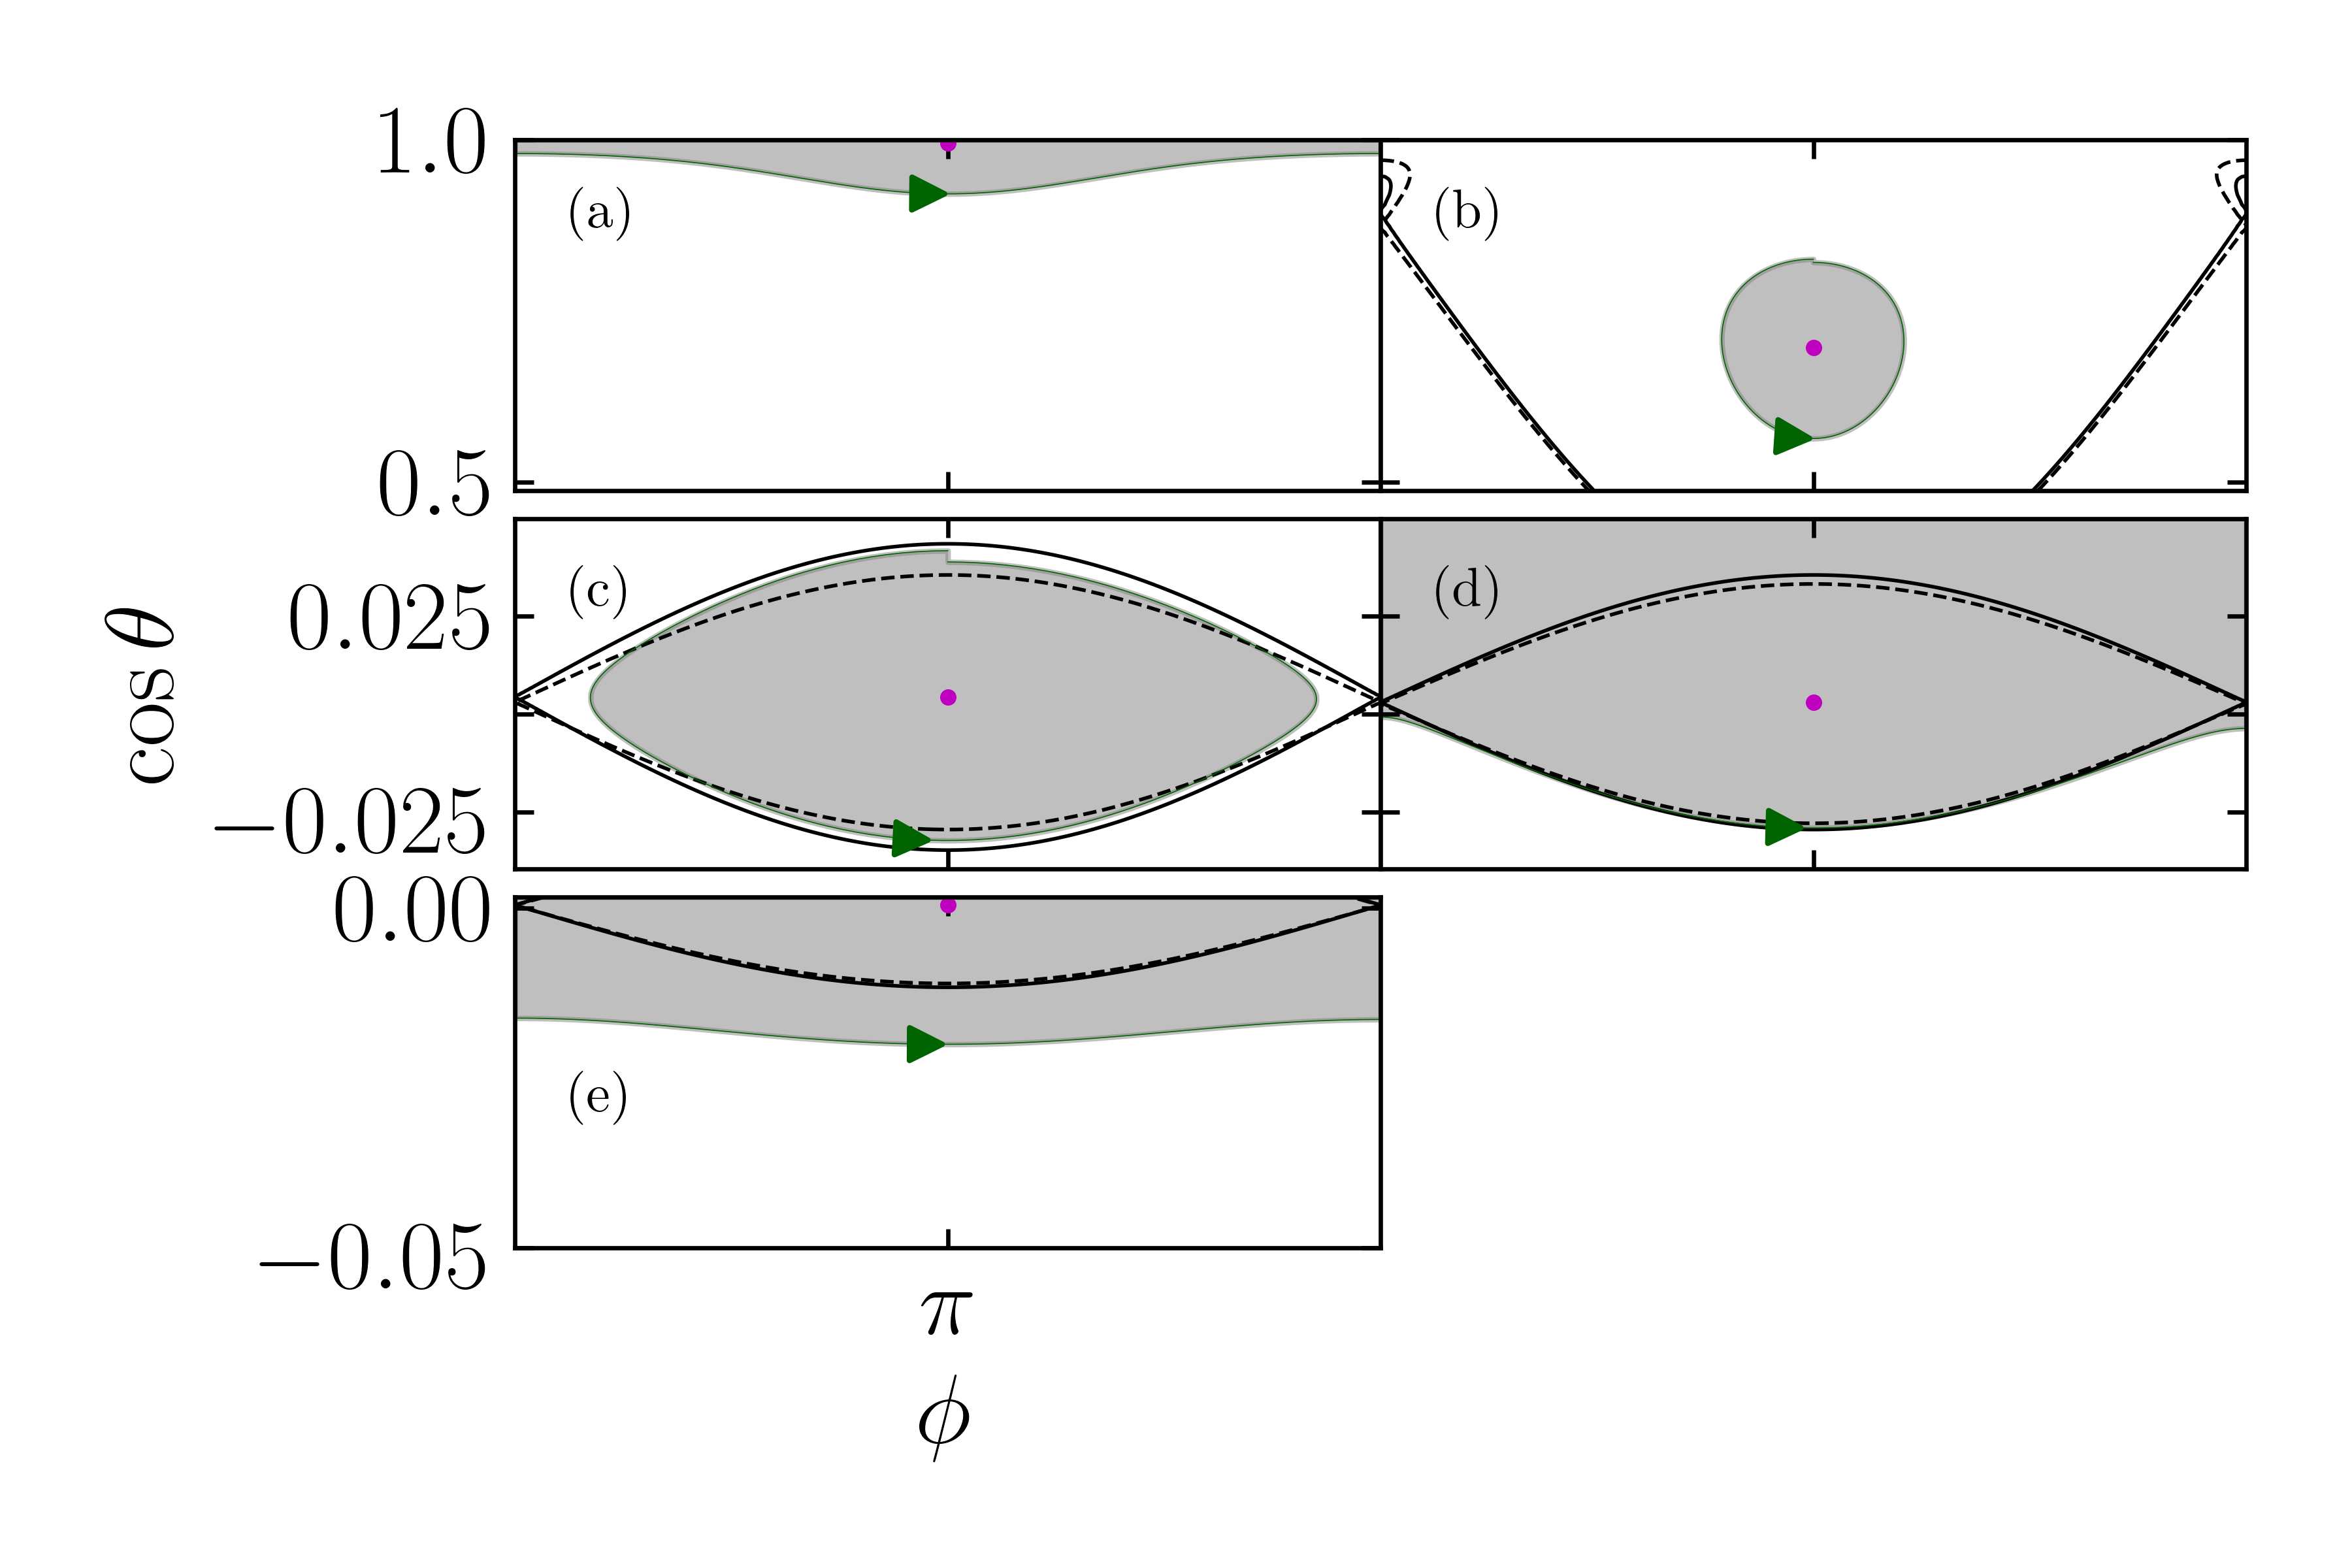
\includegraphics[width=0.5\textwidth]{../initial/2_toy2/3testo23_subplots.png}
    \end{subfigure}
    \caption{Same as Fig.~\ref{fig:ad_21} but for the $A_2 \to A_3$ track.
    $\theta_{\rm sd, i} = 0.3\;\mathrm{rad}$ and $\epsilon = 3.01 \times
    10^{-4}$.}\label{fig:ad_23}
\end{figure}
\begin{figure}
    \centering
    \begin{subfigure}{\columnwidth}
        \centering
        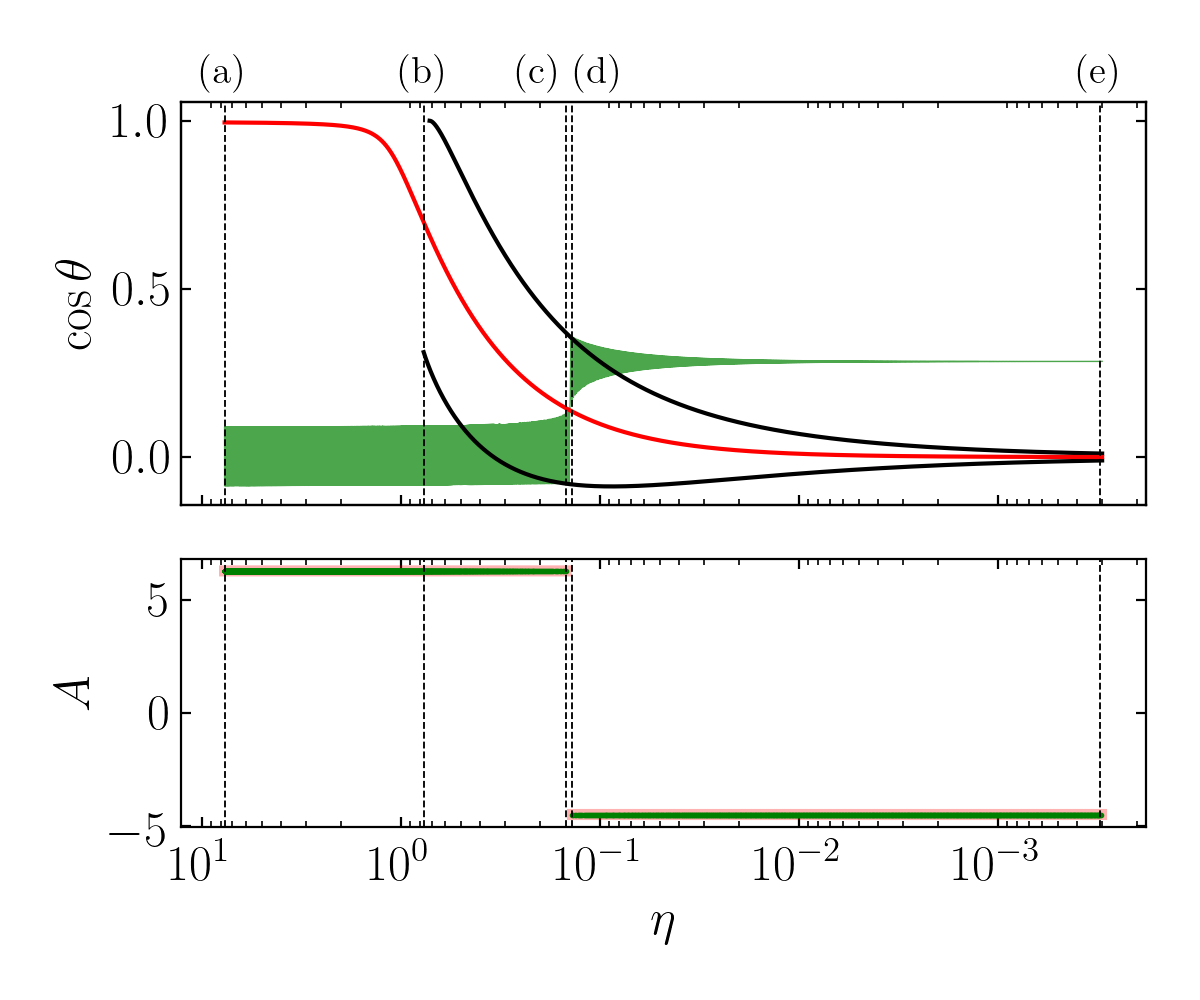
\includegraphics[width=0.5\textwidth]{../initial/2_toy2/3testo31.png}
    \end{subfigure}
    \begin{subfigure}{\columnwidth}
        \centering
        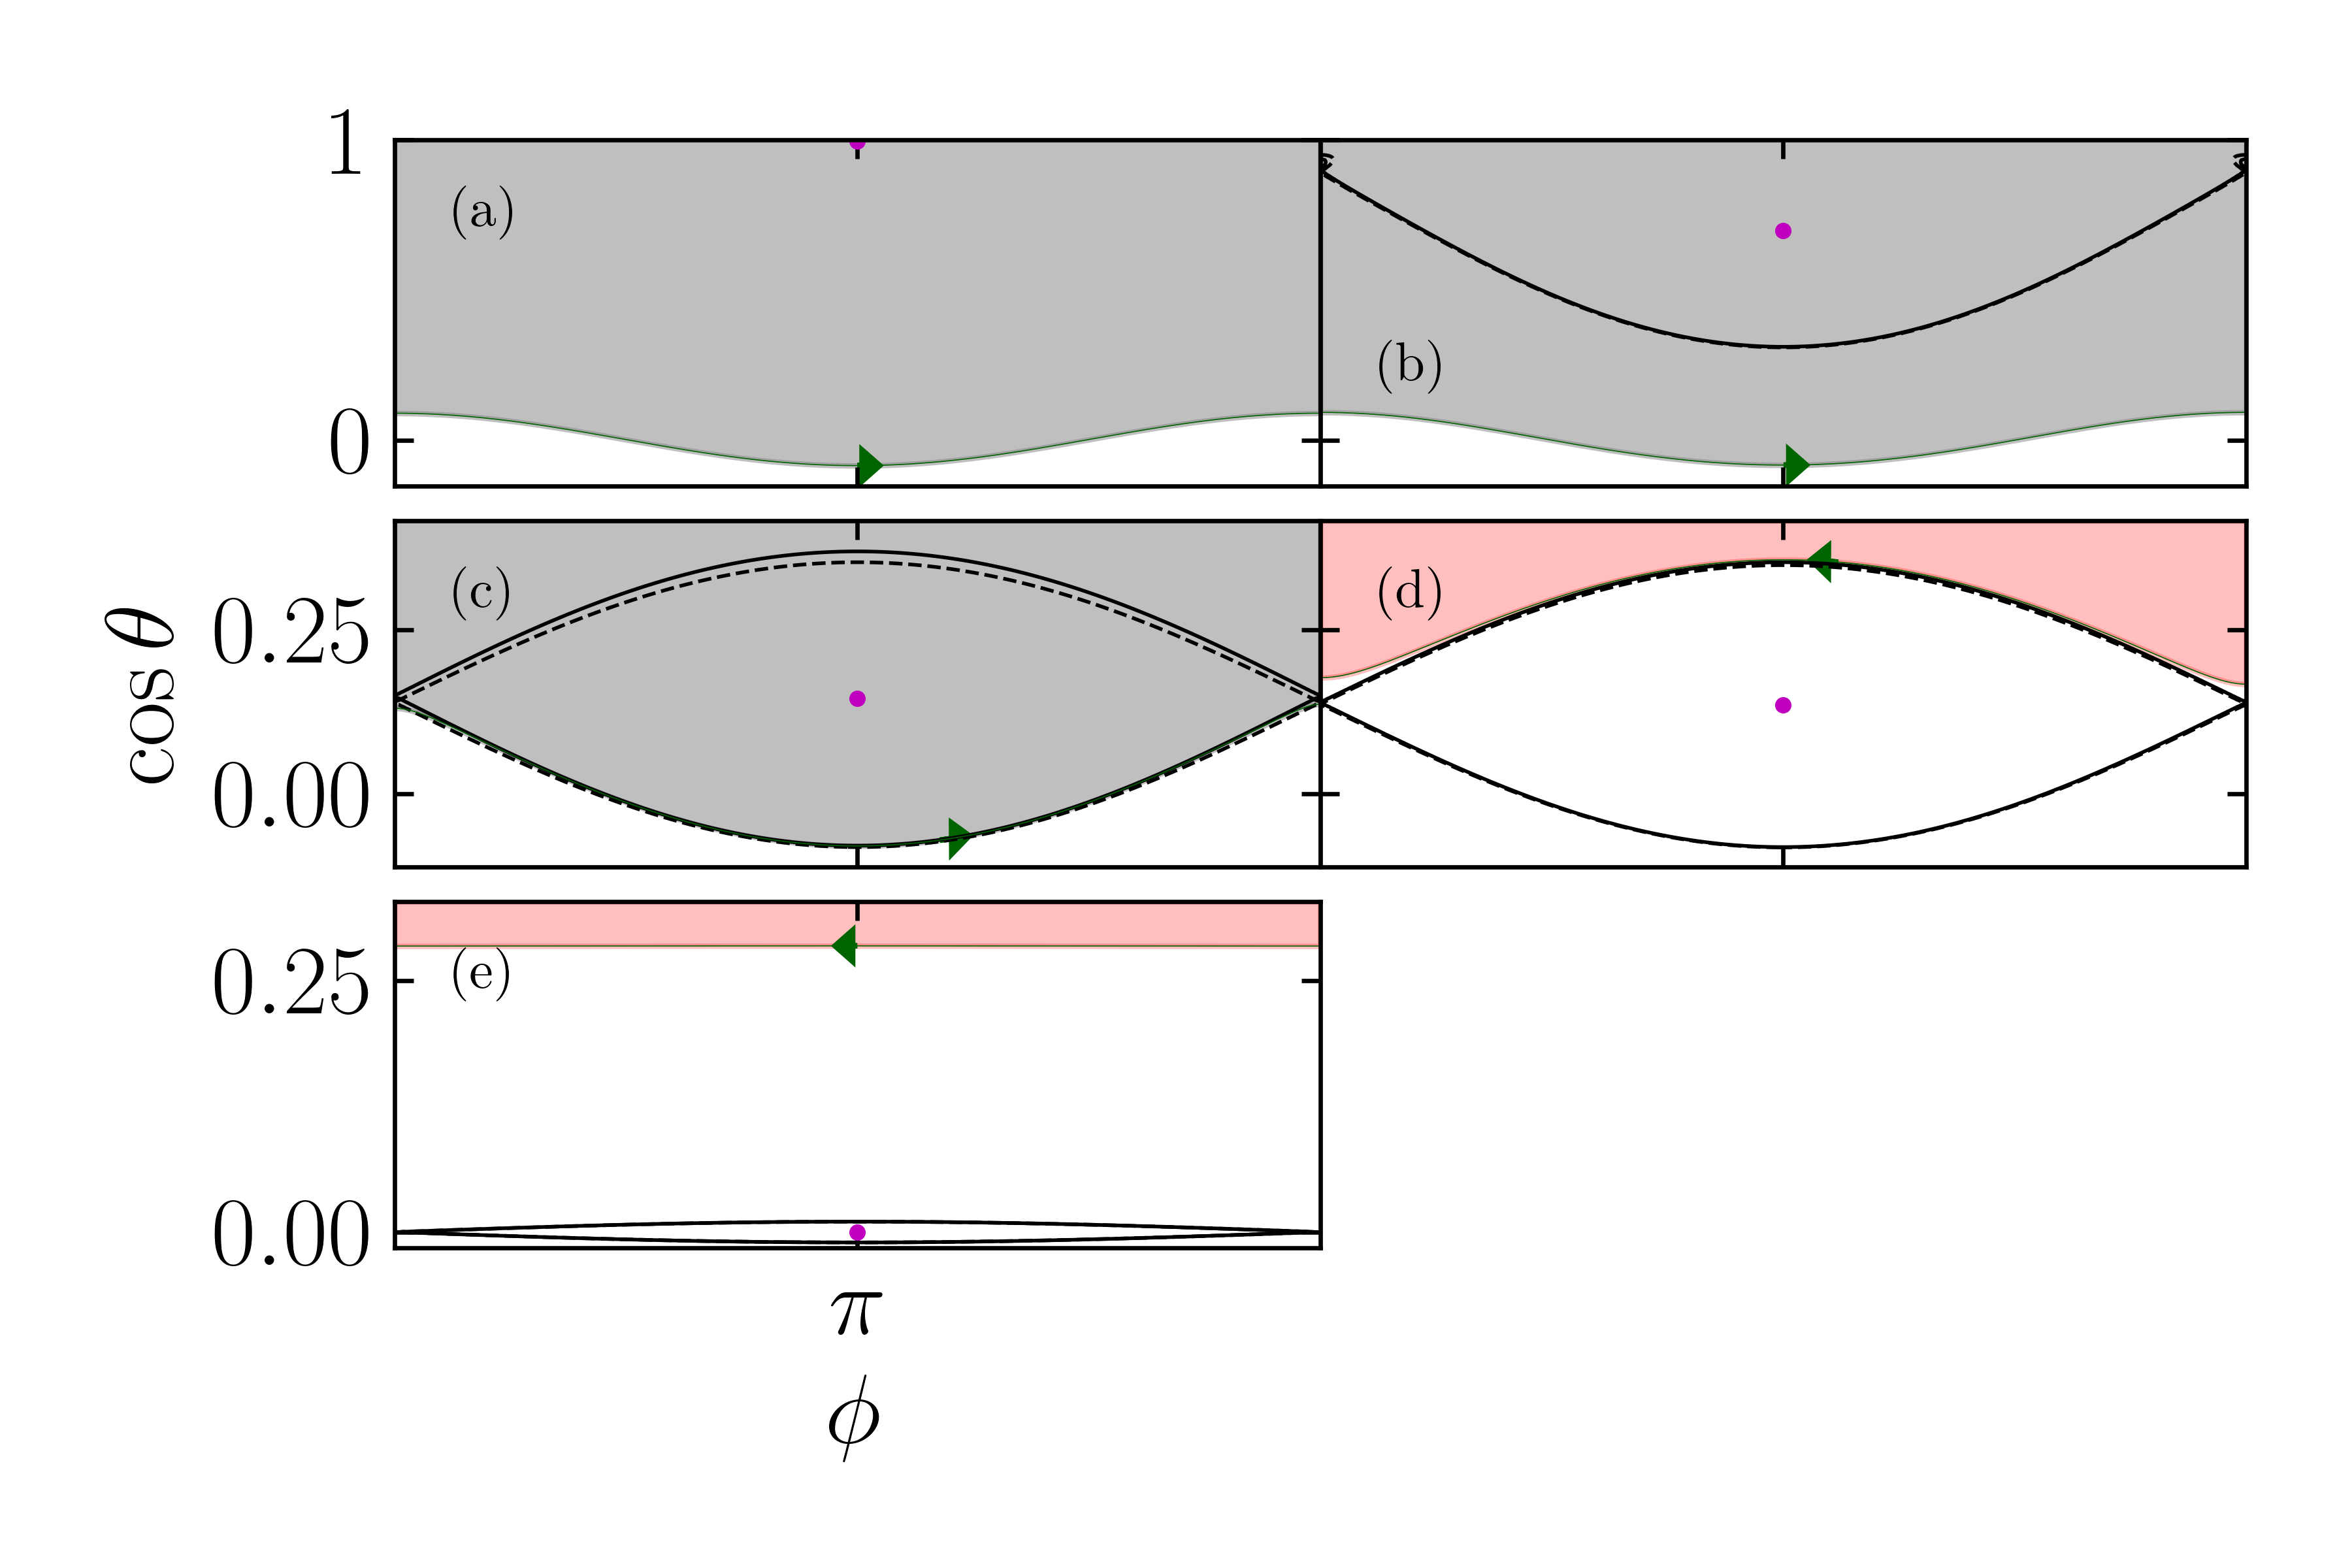
\includegraphics[width=0.5\textwidth]{../initial/2_toy2/3testo31_subplots.png}
    \end{subfigure}
    \caption{Same as Fig.~\ref{fig:ad_21} but for the $A_{\rm III} \to A_{\rm I}$
    track. $\theta_{\rm sd, i} = 89.1^\circ$, and $\epsilon = 3 \times
    10^{-4}$.}\label{fig:ad_31}
\end{figure}
\begin{figure}
    \centering
    \begin{subfigure}{\columnwidth}
        \centering
        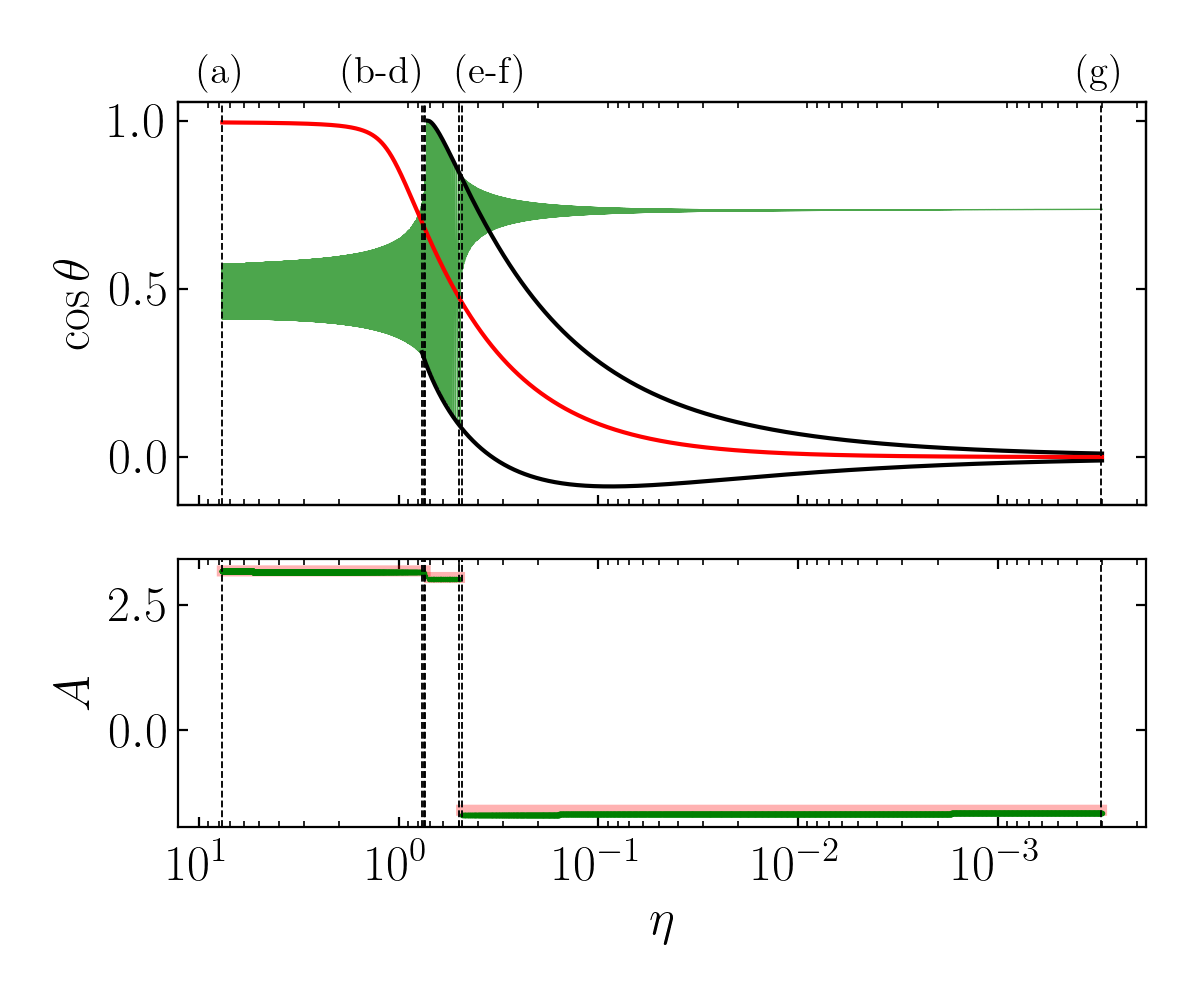
\includegraphics[width=0.5\textwidth]{../initial/2_toy2/3testo321.png}
    \end{subfigure}
    \begin{subfigure}{\columnwidth}
        \centering
        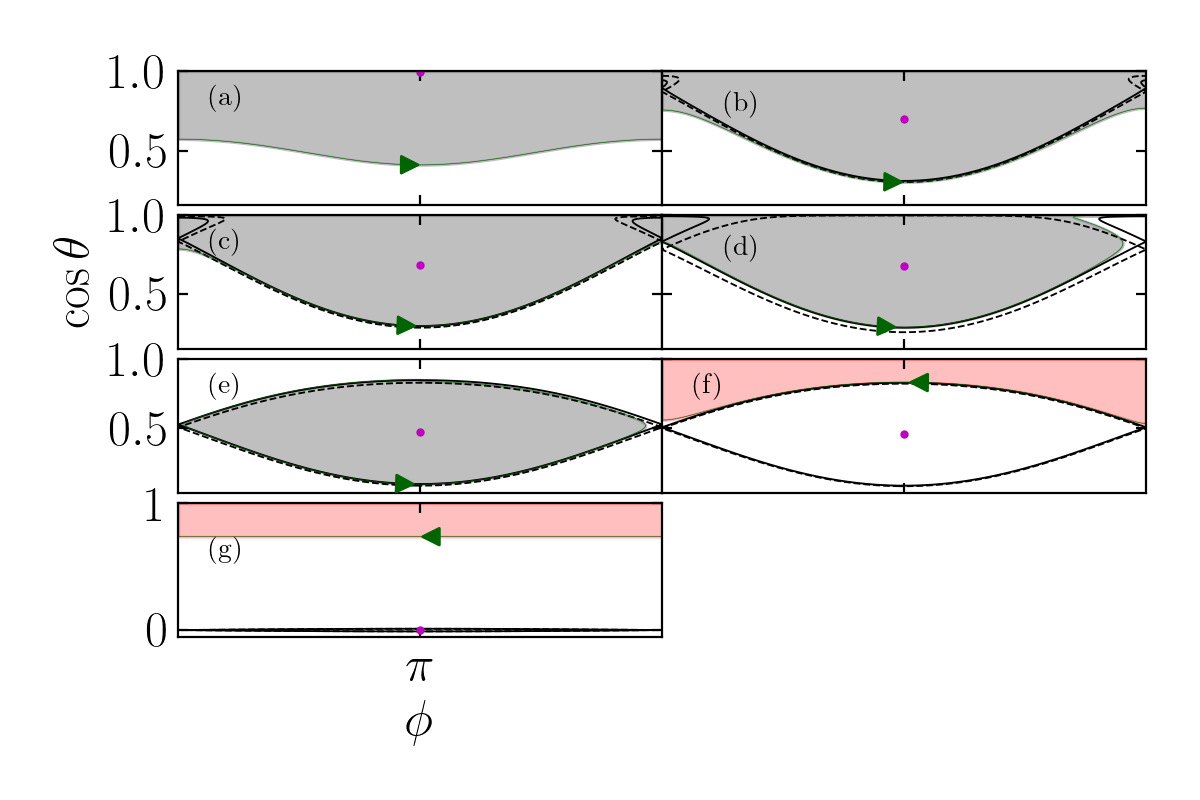
\includegraphics[width=0.5\textwidth]{../initial/2_toy2/3testo321_subplots.png}
    \end{subfigure}
    \caption{Same as Fig.~\ref{fig:ad_21} but for the $A_{\rm III} \to A_{\rm II}
    \to A_{\rm I}$ track. $\theta_{\rm sd, i} = 60^\circ$, and $\epsilon = 3.14
    \times 10^{-4}$. Two separatrix crossings are shown.}\label{fig:ad_321}
\end{figure}

\section{Nonadiabatic Effects}\label{s:nonad}

\subsection{Transition to Non-adiabaticity}\label{ss:transition}

To illustrate the transition to non-adiabaticity, we present below two
simulations with larger $\epsilon$ than used for Fig.~\ref{fig:ad_ensemble} in
Figs.~\ref{fig:3_ensemble_05_25} and~\ref{fig:3_ensemble_05_15}.

At first non-adiabaticity manifests as a larger scatter of final obliquities
near the tracks predicted from adiabatic evolution. These scatters first set in
for trajectories starting in zone III, as these cross the separatrix at higher
values of $\theta$ and have a stricter adiabaticity criterion (see
Eq.~\eqref{eq:ad_constr}).

Later, these large scatters take on band-like structures that seem to persist
across values of $\theta_{\rm sd, i}$; we attribute these to the separatrix
crossing process becoming sensitive to the \emph{phase} of the final
libration/circulation orbit at separatrix crossing, which implies that $\eta$
changes substantially over the separatrix crossing orbit. This is clearly a
non-adiabatic effect but is permitted by the weak adiabaticity criterion,
which only compares $\eta$ evolution to dynamics far from the separatrix.
\begin{figure}
    \centering
    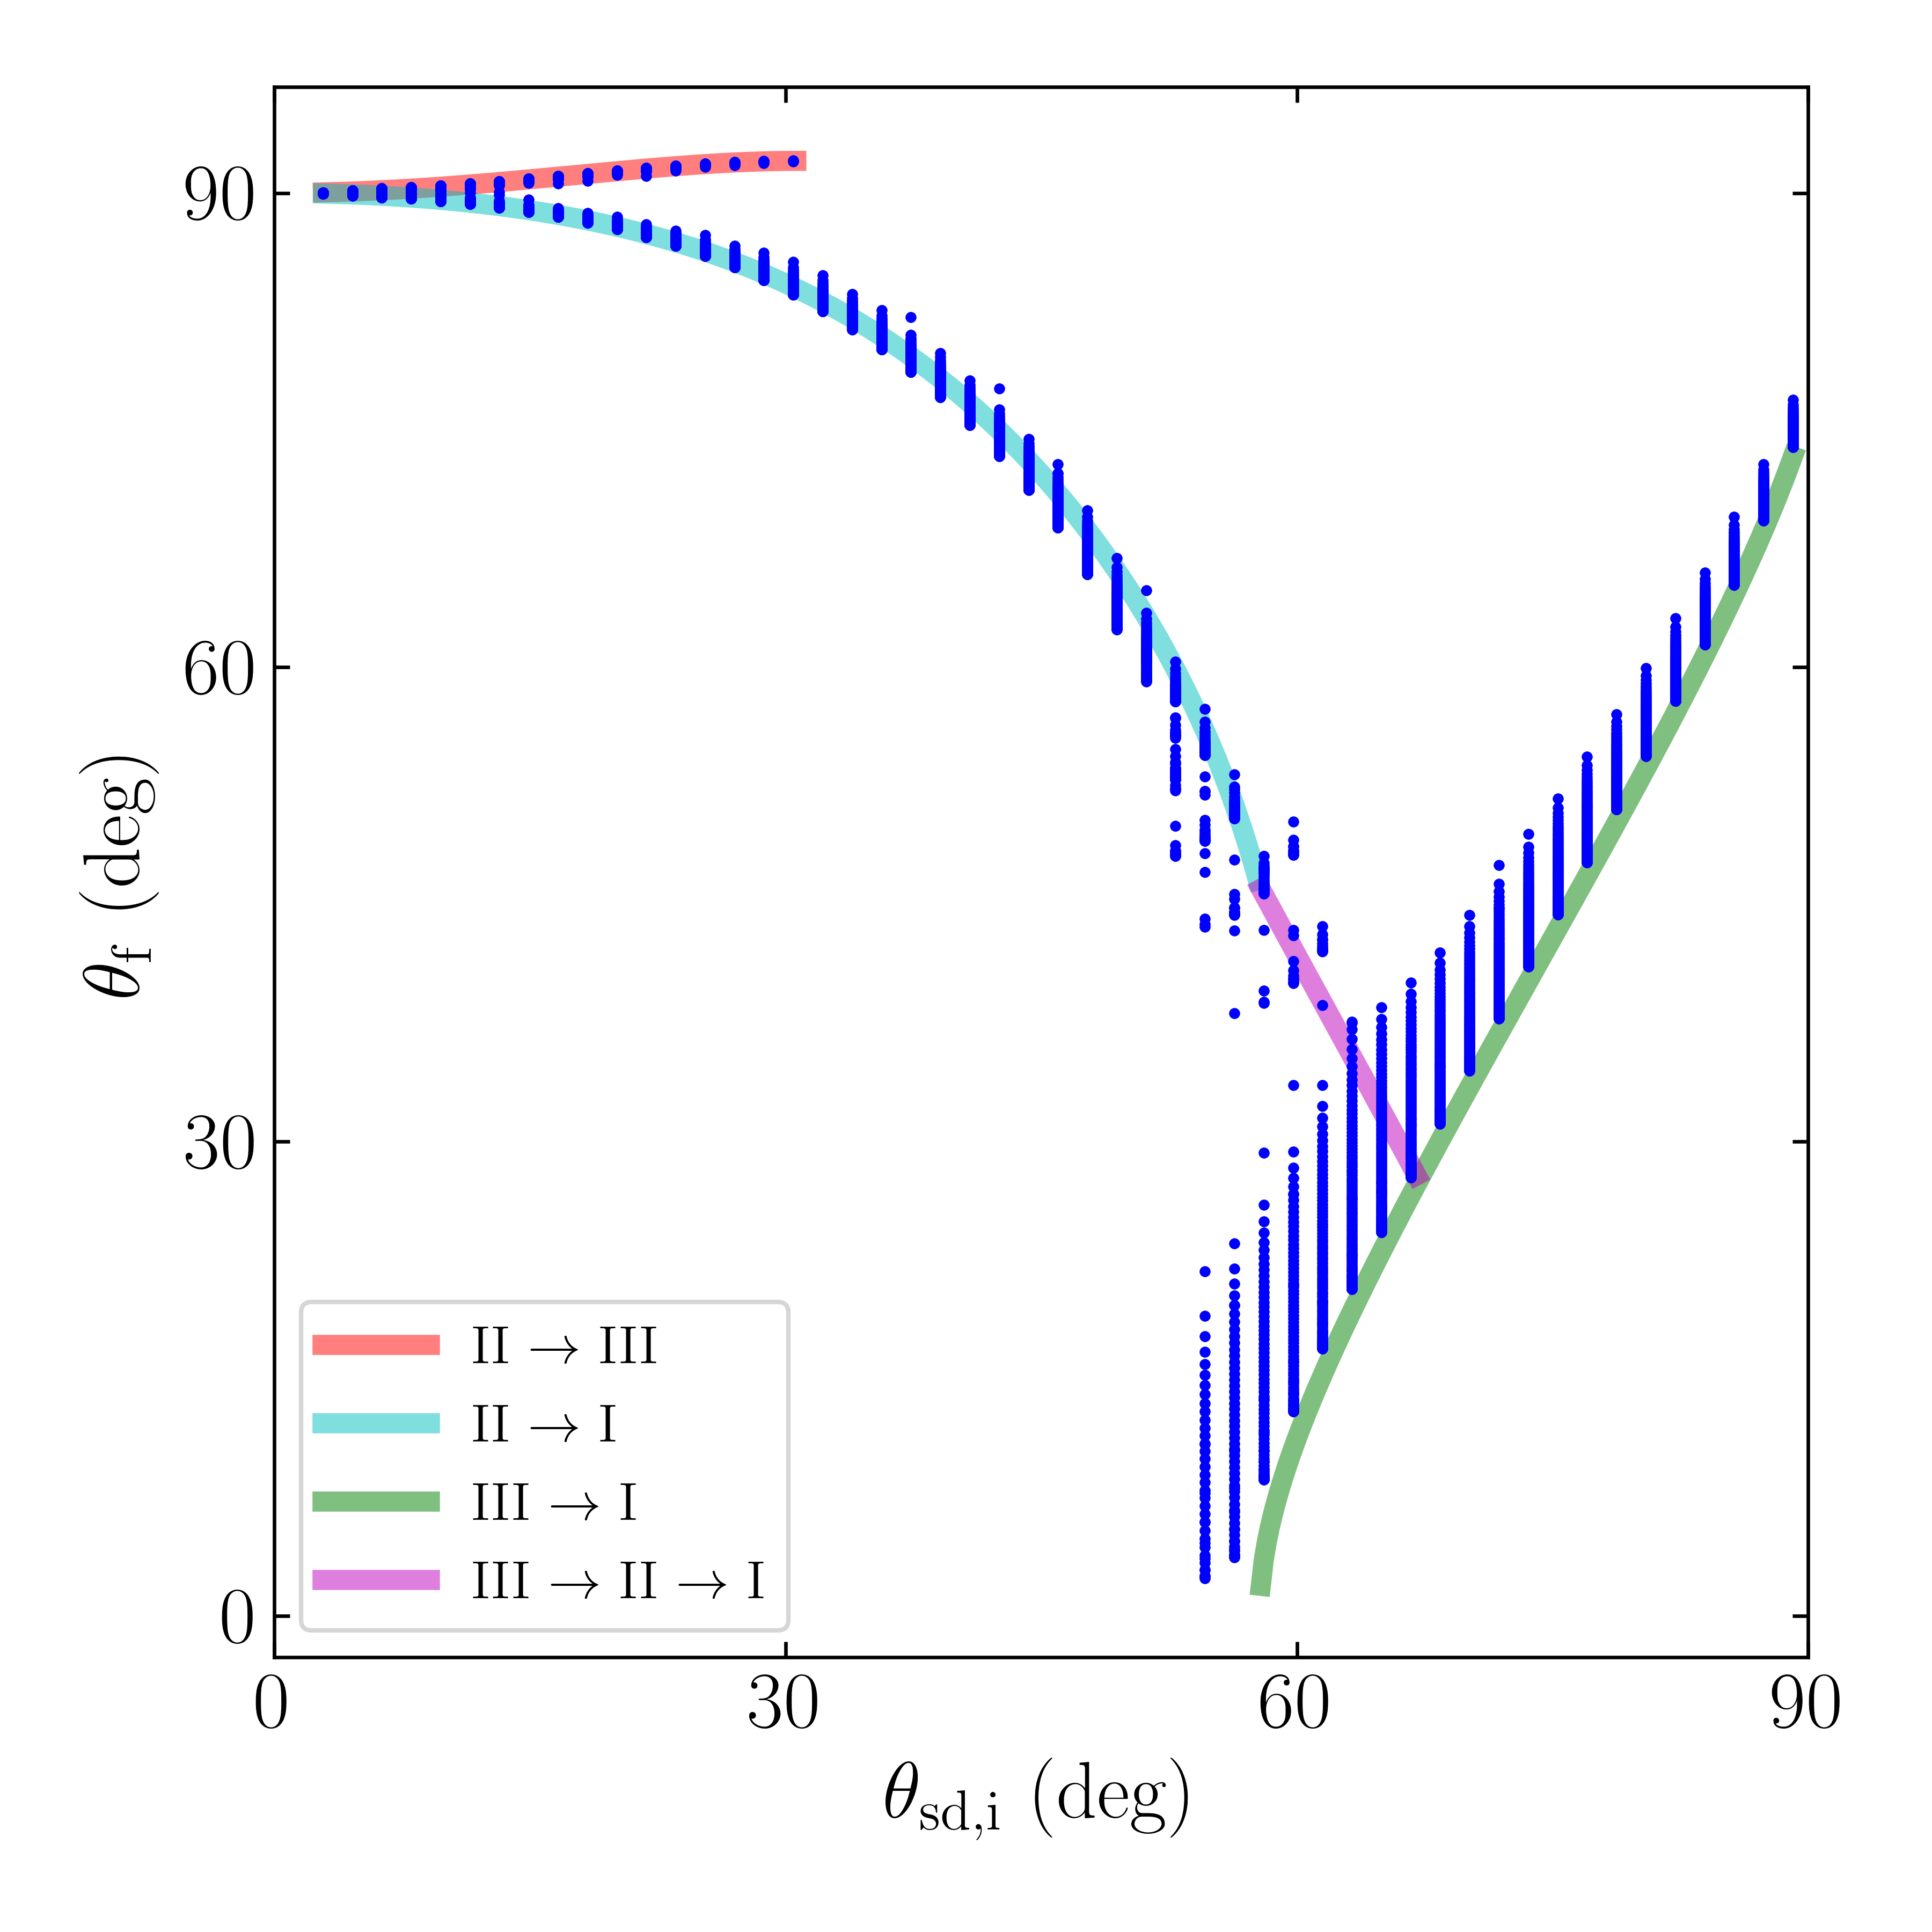
\includegraphics[width=0.5\textwidth]{../initial/2_toy2/3_ensemble_05_25.png}
    \caption{Same as Fig.~\ref{fig:ad_ensemble} but for $\epsilon = 10^{-2.5}$,
    and restricting $\theta_{\rm sd, i} < 90^\circ$. A larger spread from the
    dynamical tracks is observed in the data.}\label{fig:3_ensemble_05_25}
\end{figure}
\begin{figure}
    \centering
    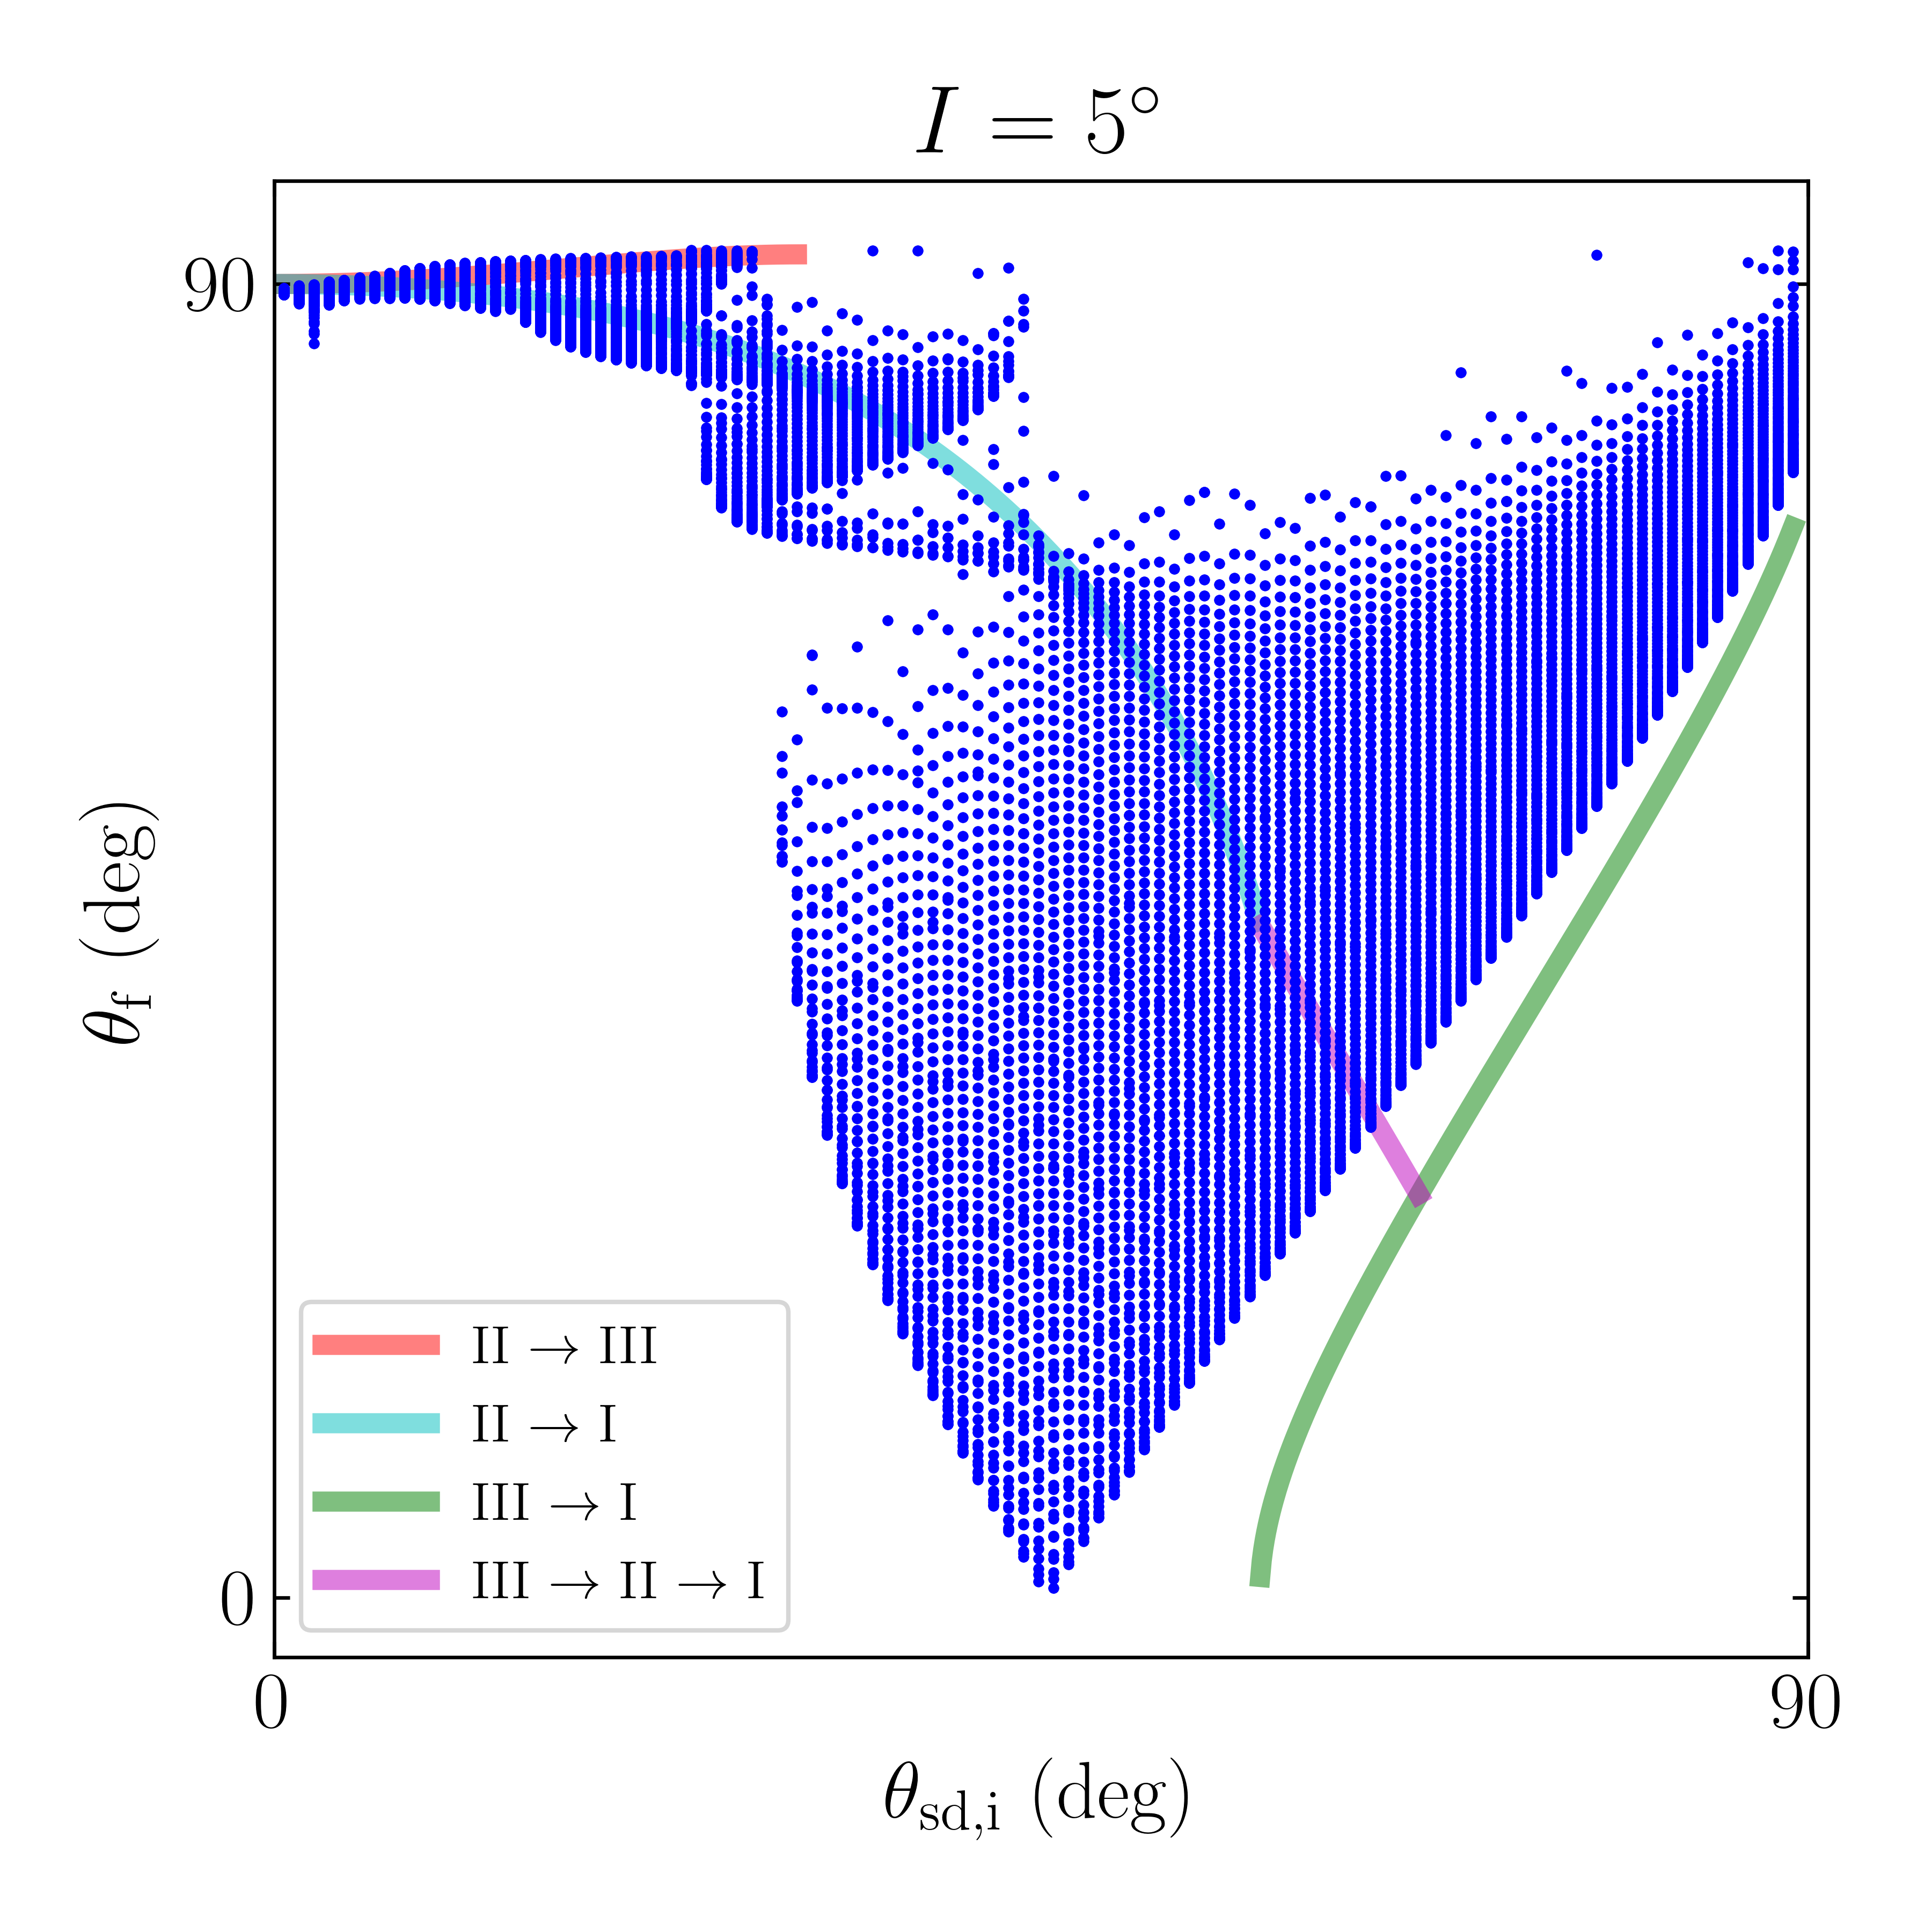
\includegraphics[width=0.5\textwidth]{../initial/2_toy2/3_ensemble_05_15.png}
    \caption{Same as Fig.~\ref{fig:3_ensemble_05_25} but for $\epsilon =
    10^{-1.5}$. Some small semblance of the evolutionary tracks remains, and the
    deviations appear to have a banded structure. This can be attributed to
    non-adiabaticity ``freezing-in'' the phase of the obliquity variations over
    the final libration/circulation orbit prior to separatrix
    crossing.}\label{fig:3_ensemble_05_15}
\end{figure}

A sample trajectory following in the style of Fig.~\ref{fig:ad_21} but for
$\epsilon = 0.3$ (violating even weak adiabaticity) is provided in
Fig.~\ref{fig:nonad_traj}. It is clear the trajectory does not track level curves
of the Hamiltonian during each individual snapshot (e.g.\ the third snapshot).
This manifests when CS2 migrates more quickly than the trajectory can librate
about CS2, precisely a violation of the weak adiabaticity criterion.
\begin{figure}
    \centering
    \begin{subfigure}{\columnwidth}
        \centering
        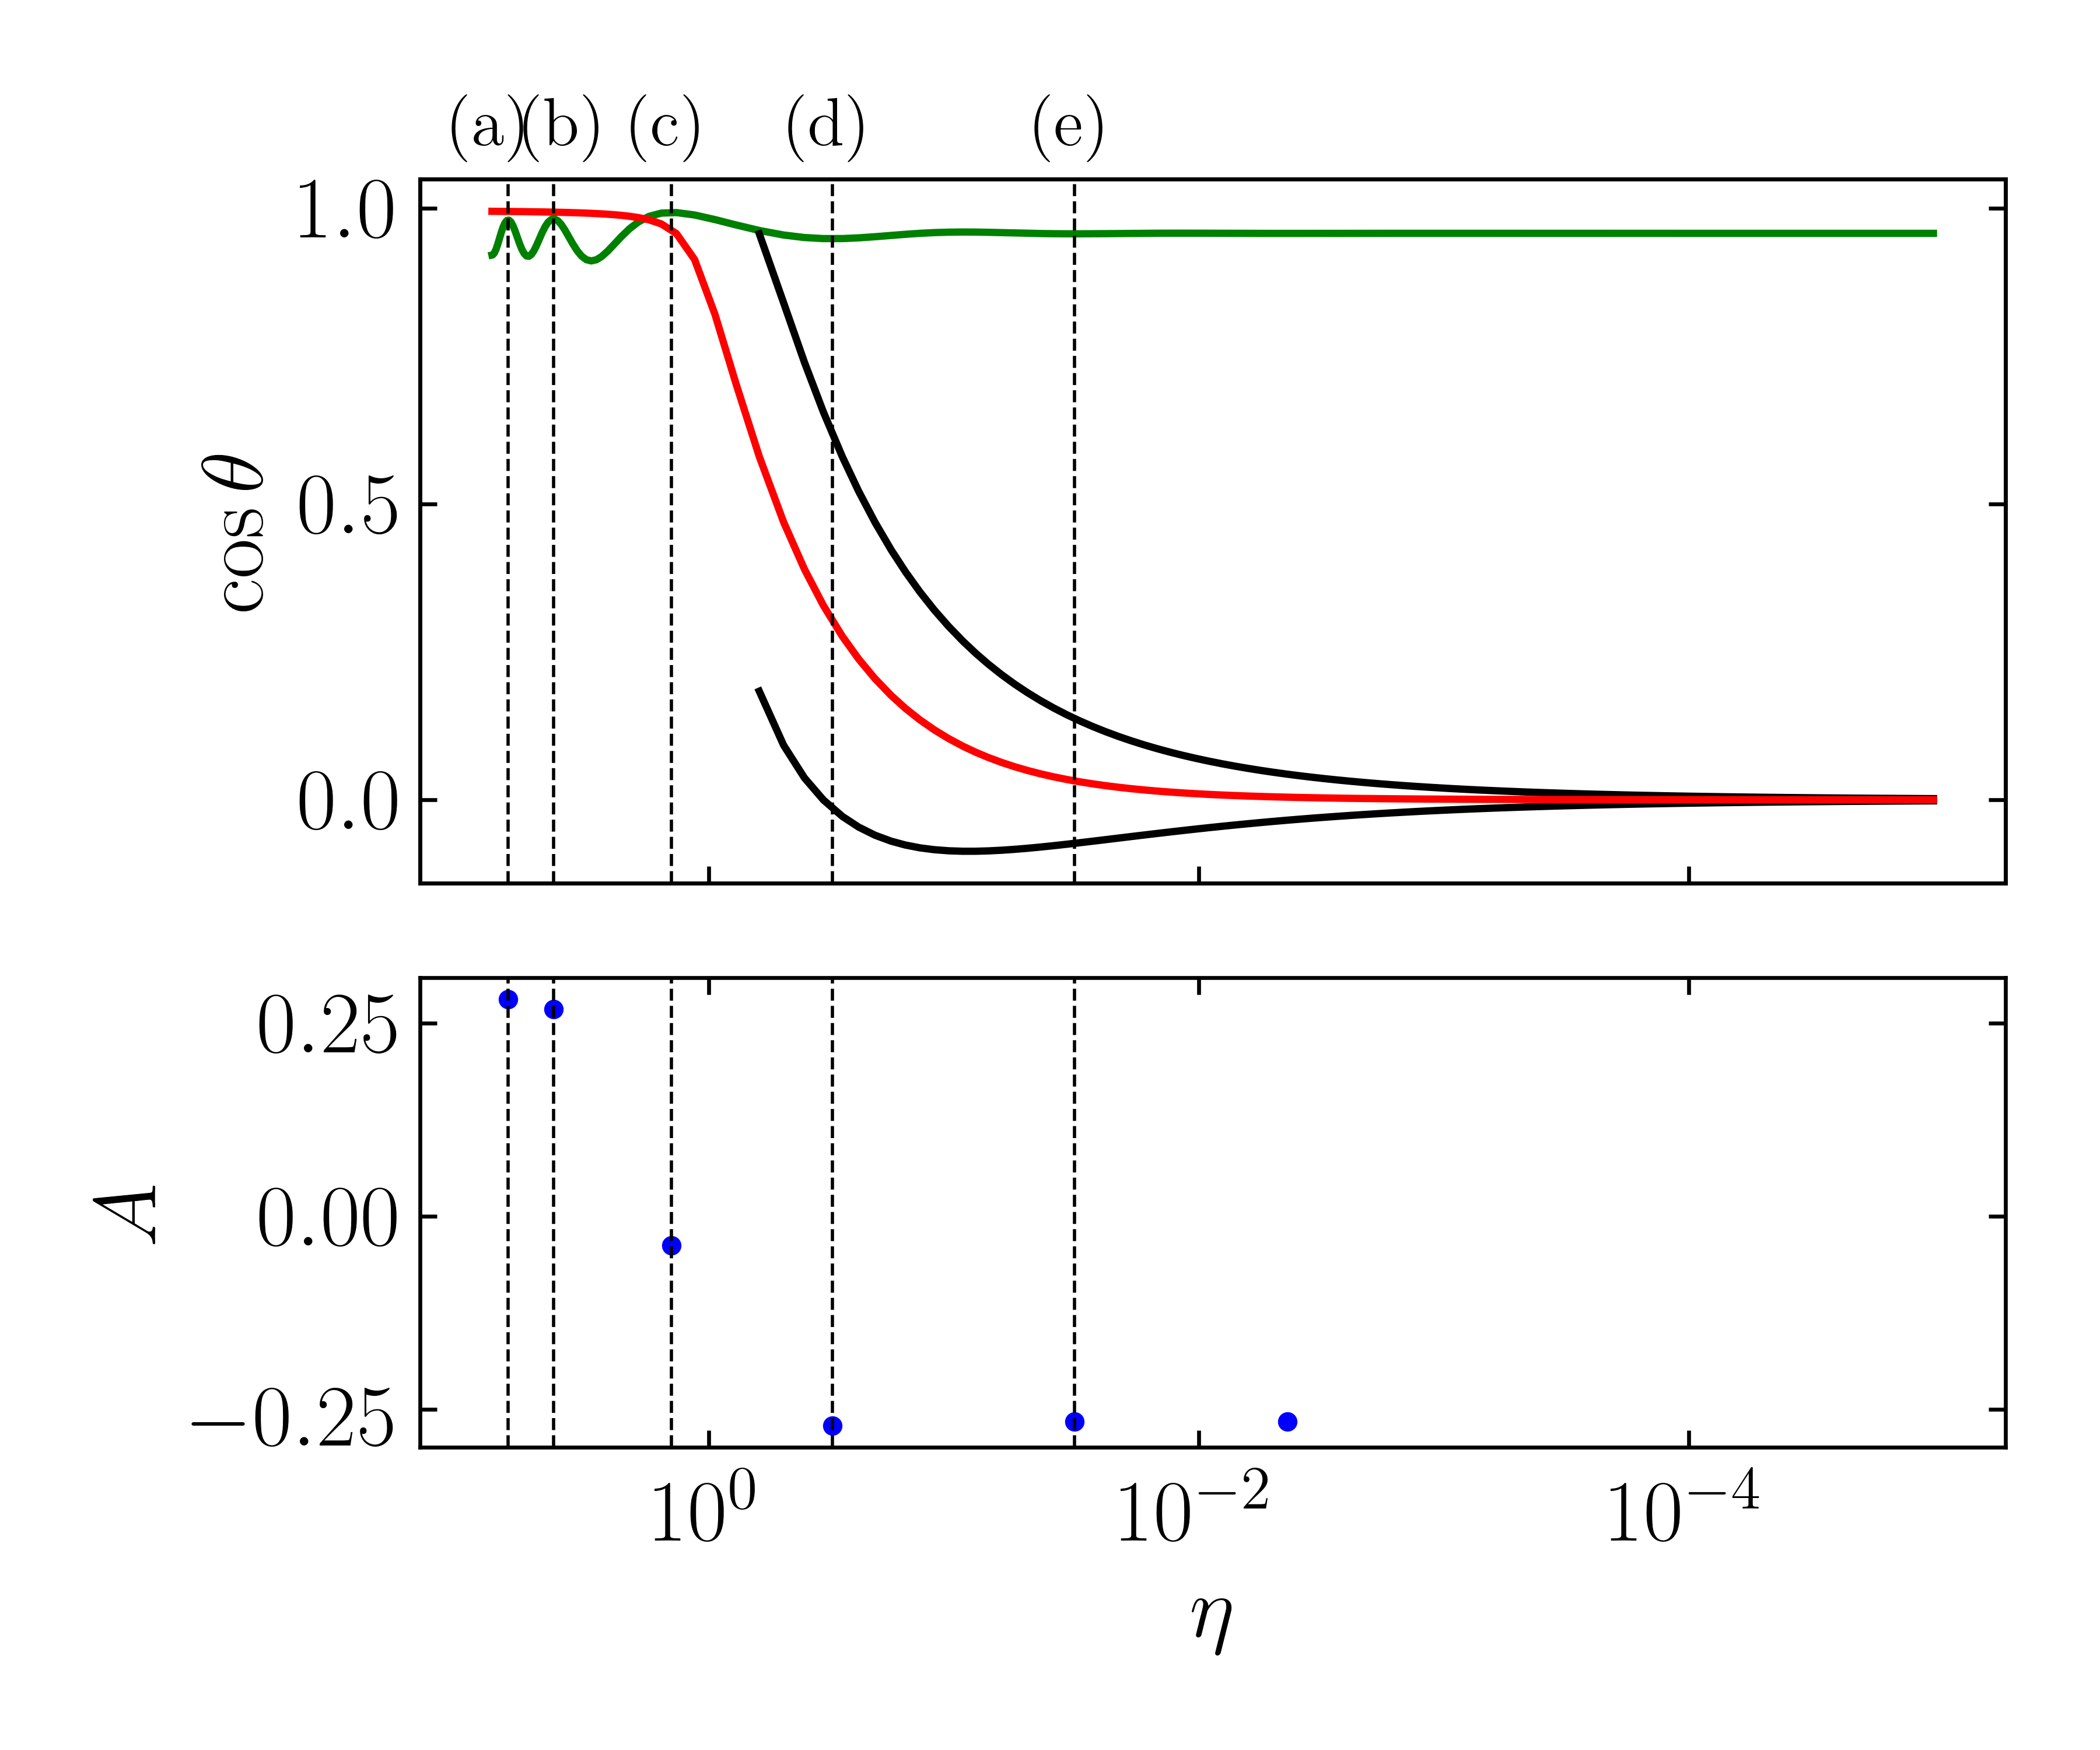
\includegraphics[width=0.5\textwidth]{../initial/2_toy2/3testo_nonad.png}
    \end{subfigure}
    \begin{subfigure}{\columnwidth}
        \centering
        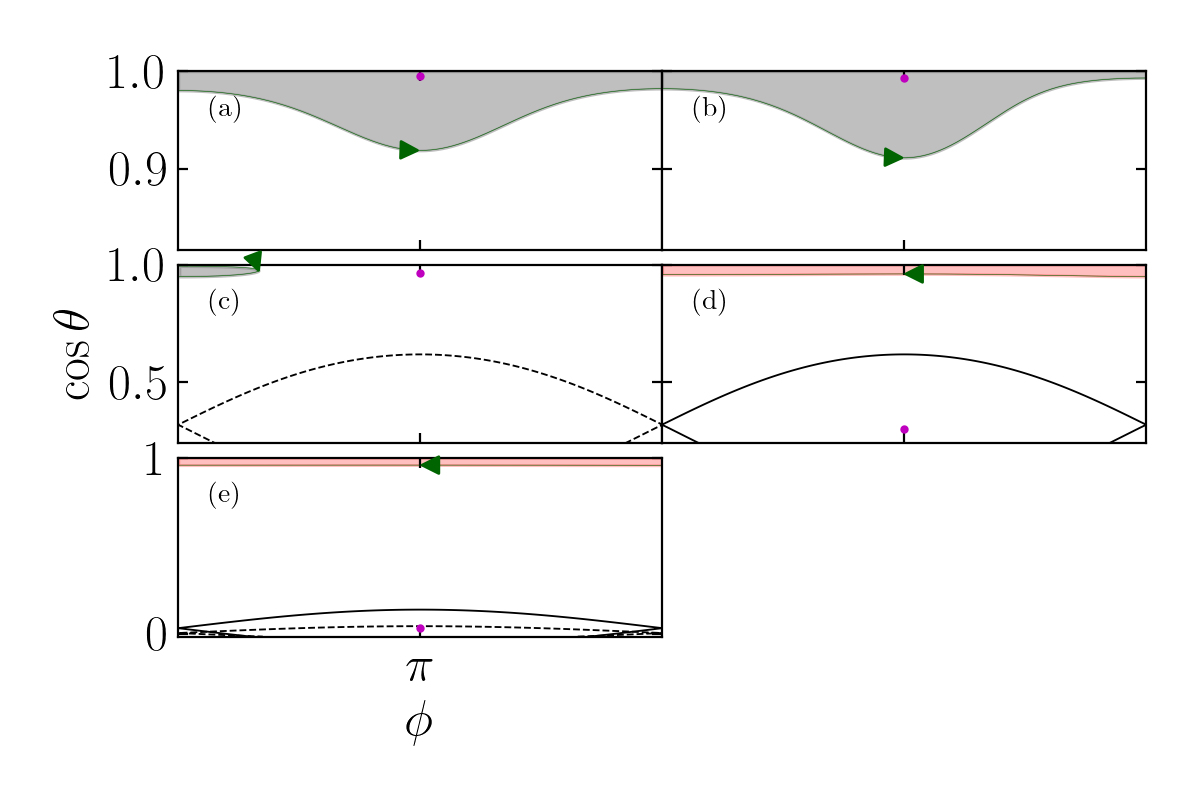
\includegraphics[width=0.5\textwidth]{../initial/2_toy2/3testo_nonad_subplots.png}
    \end{subfigure}
    \caption{Same as Fig.~\ref{fig:ad_21} but for a non-adiabatic $\epsilon =
    0.3$. In the top panel of the top plot, it is evident that the libration
    cycle about CS2 is unable to keep up with the swift motion of CS2 as $\eta$
    changes, decreasing the obliquity jump. In the bottom plot, we can see that
    individual orbits do not lie along level curves of the Hamiltonian, as the
    Hamiltonian phase space changes quickly compared to the period of
    circulation cycles.}\label{fig:nonad_traj}
\end{figure}

\subsection{Non-adiabatic Evolution Outcomes}

We now consider the general problem of how a state evolves when $\eta$ changes
non-adiabatically. In Appendix~\ref{s:ad_approx}, we derive a formula for
$\theta_{\rm f}$ assuming no initial spin-disk misalignment:
\begin{equation}
    \theta_{\rm f}\p{\theta_{\rm sd, i} = 0} = \sqrt{\frac{2\pi}{\epsilon}} \tan
        I\cos I.\label{eq:nonad_q_f}
\end{equation}

An intuitive guess at generalizing this assumes that any nonzero $\theta_{\rm
sd, i}$ manifests as obliquity variations as $\uv{s}$ librates about
$\uv{l}_{\rm d}$. These can be accounted for by simply allowing the final
obliquity to vary over the same range as the initial obliquity, or,
\begin{equation}
    \theta_{\rm f}\p{\theta_{\rm sd, i}} - \sqrt{\frac{2\pi}{\epsilon}} \tan
        I\cos I\in \s{-\theta_{\rm sd, i}, \theta_{\rm sd,i}}
        .\label{eq:nonad_q_f_dist}
\end{equation}
In Fig.~\ref{fig:nonad_3_ensemeble}, we show that this proves a remarkably
accurate when taking $\epsilon = 0.3$.
\begin{figure}
    \centering
    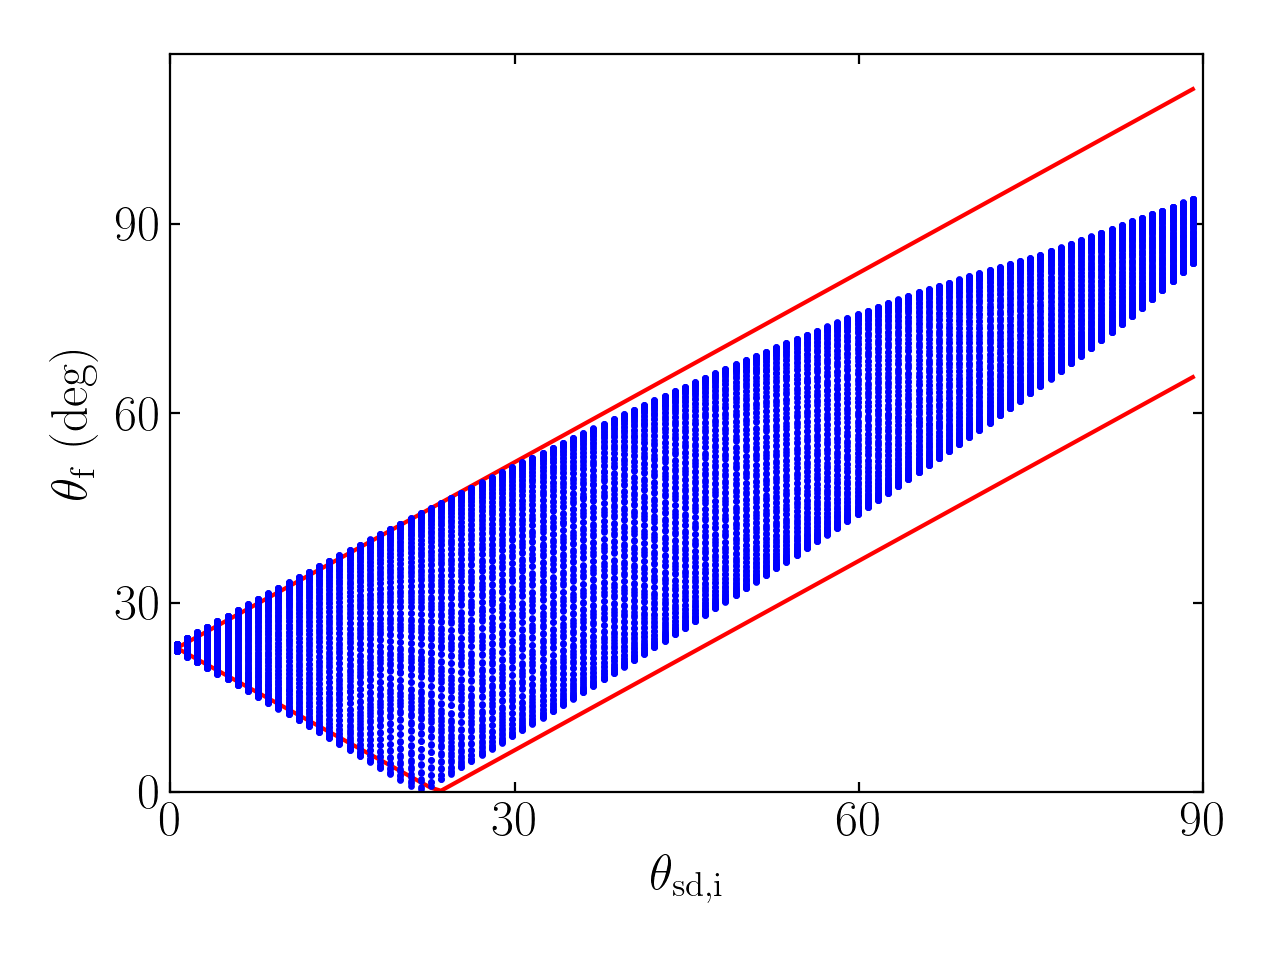
\includegraphics[width=0.5\textwidth]{../initial/2_toy2/3_ensemble_05_05.png}
    \caption{$\theta_{\rm  f}\p{\theta_{\rm sd, i}}$ at $\epsilon = 0.3$, firmly
    in the non-adiabatic regime. Note the clear double-valuedeness has
    disappeared, as have distinct dynamical tracks. The red dotted line presents
    the analytical prediction given by
    Eq.~\eqref{eq:nonad_q_f_dist}.}\label{fig:nonad_3_ensemeble}
\end{figure}

The agreement of Eq.~\eqref{eq:nonad_q_f} at fixed I for varying $\epsilon$ is
shown in Fig.~\ref{fig:nonad_3_scan}. Note that $\epsilon \to 0$ recovers the
adiabatic regime. The deviation of $\theta_{\rm f}$ from the analytical
prediction within the adiabatic regime is indeed due to adiabatic effects
becoming dominant; compare to Fig.~\ref{fig:nonad_3_scan_20} where little
deviation is observed until $\theta_{\rm f} \approx 90^\circ$.
\begin{figure}
    \centering
    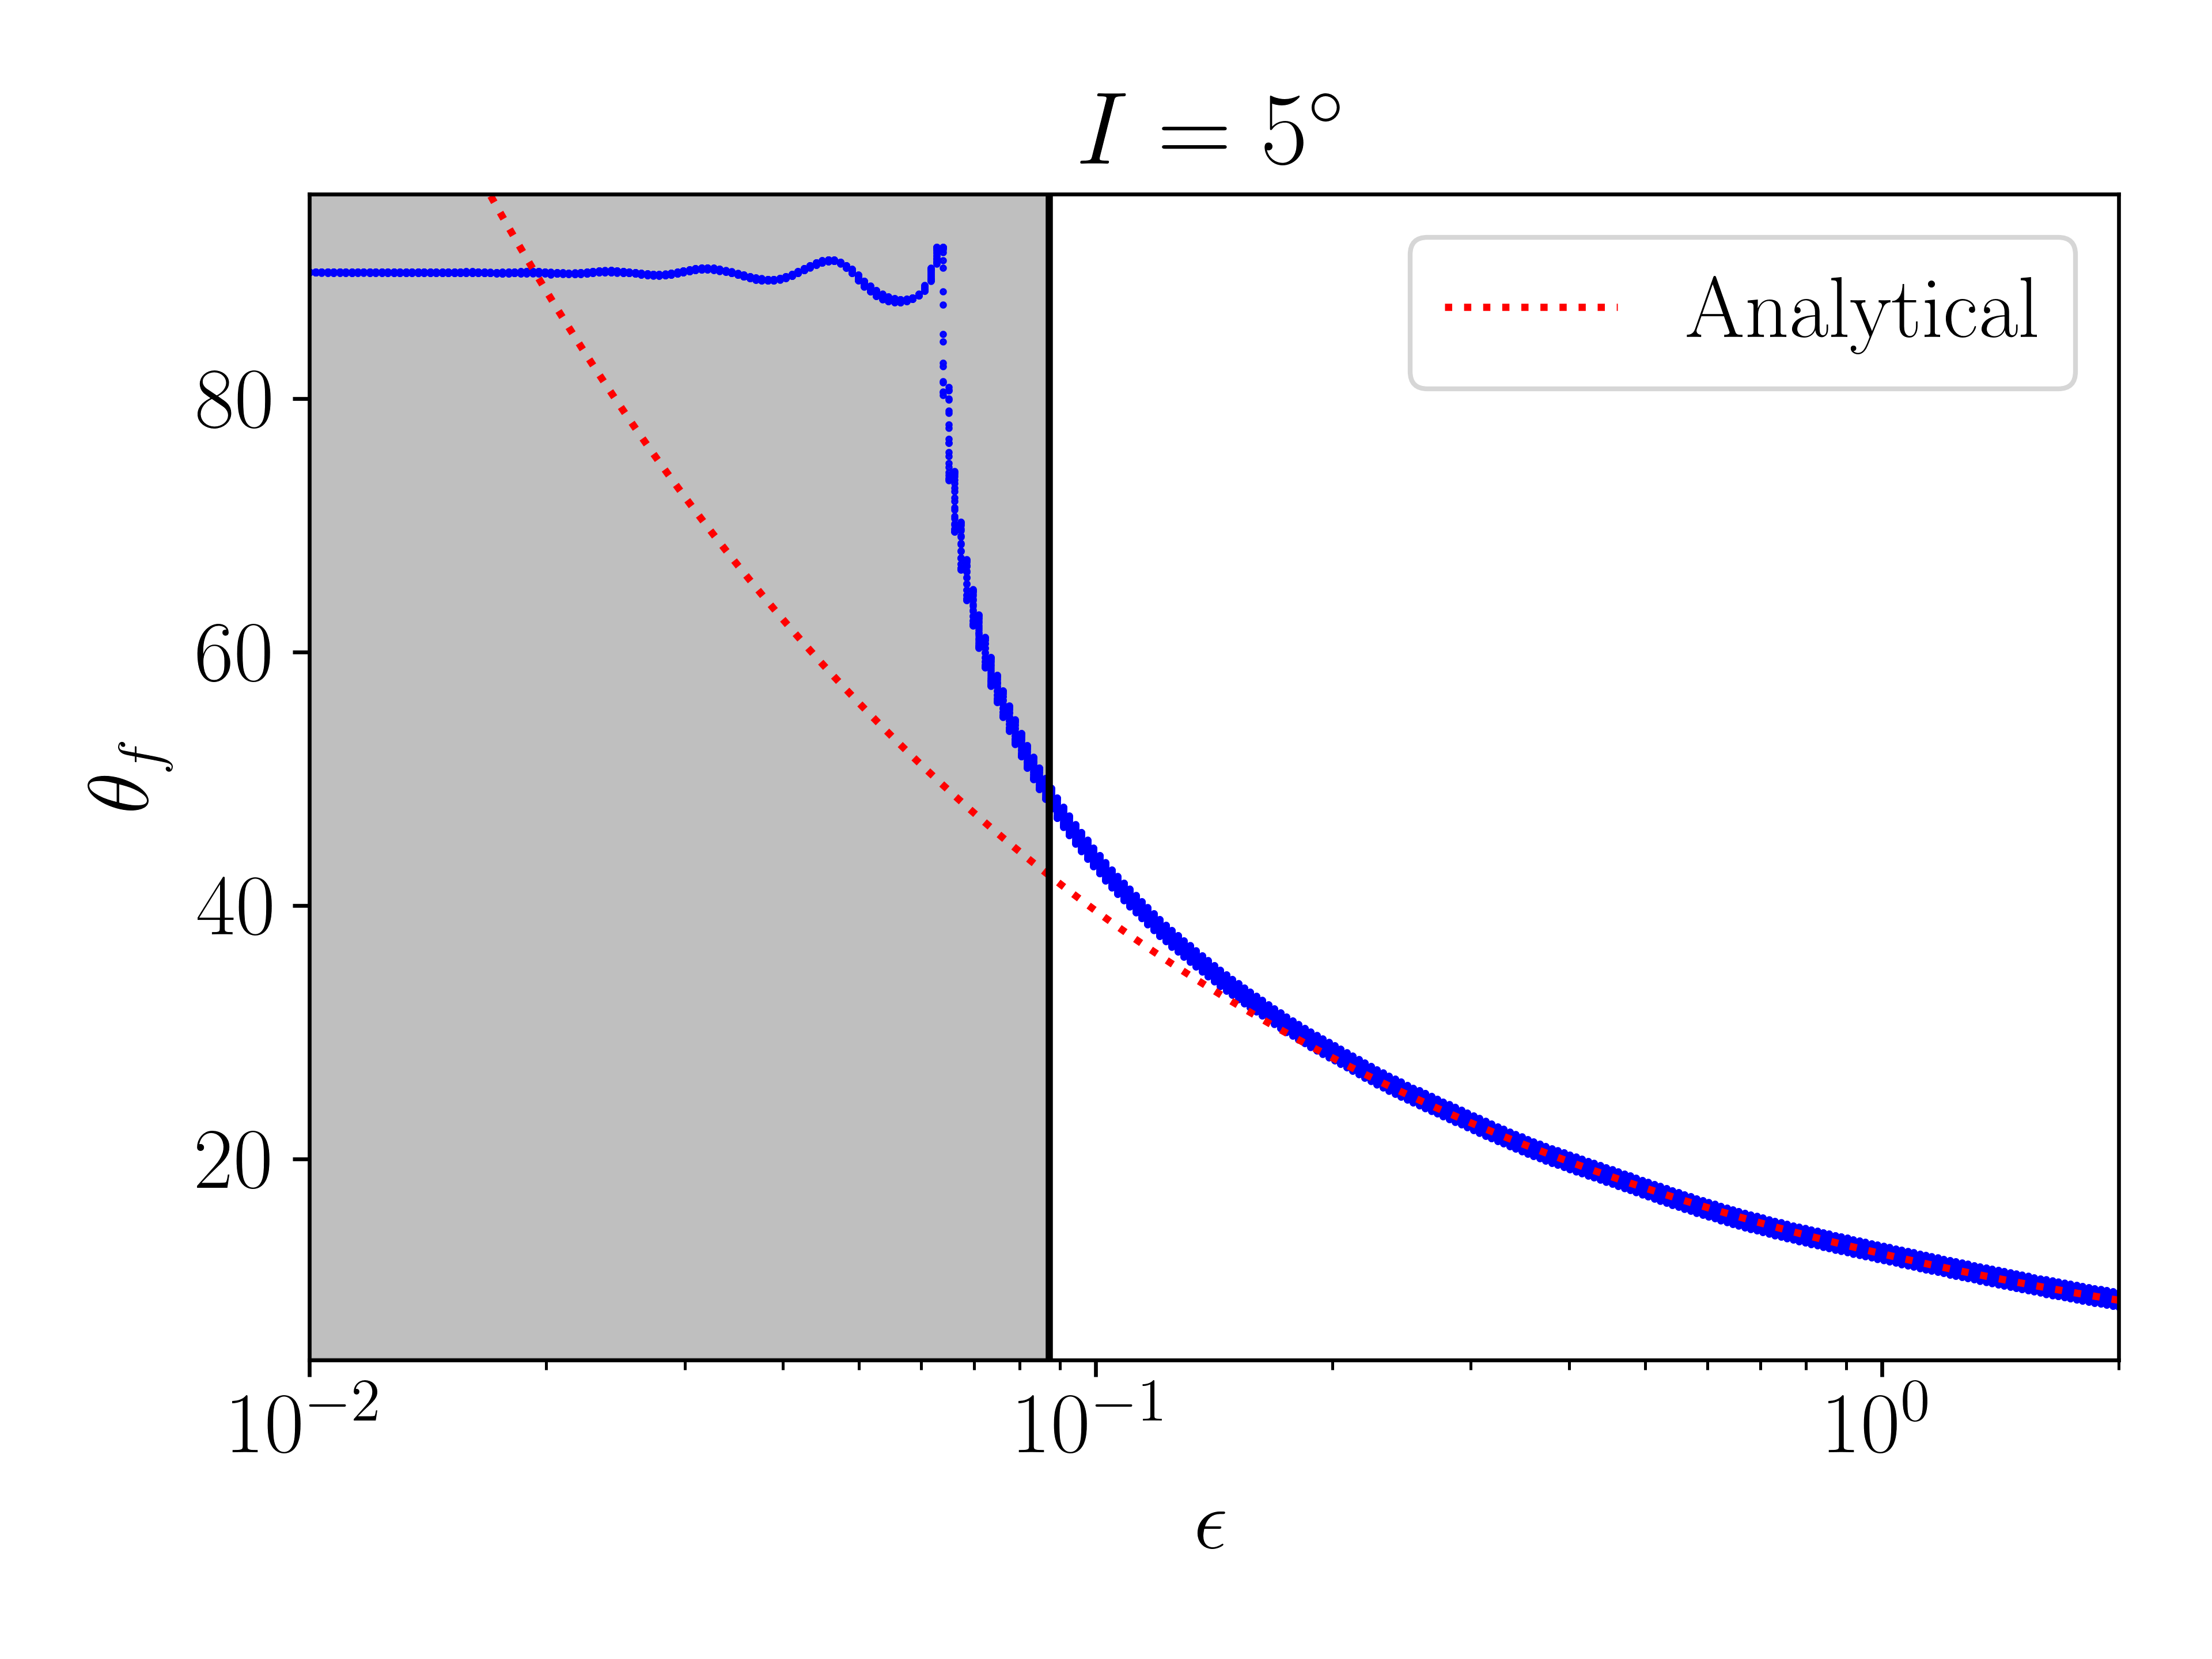
\includegraphics[width=0.5\textwidth]{../initial/2_toy2/3scan.png}
    \caption{Plot of $\theta_{\rm  f}\p{\theta_{\rm sd, i} = 0}$ as a function
    of $\epsilon$, where $I = 5^\circ$. The shaded area, bordered by the black
    line, corresponds to the adiabatic regime estimated by
    Eq.~\eqref{eq:ad_constr}. Overplotted in the red line is
    Eq.~\eqref{eq:nonad_q_f}, which is in good agreement for $\epsilon \gtrsim
    0.1$ the non-adiabatic regime, while $\theta_{\rm f} \approx 90^\circ$ in
    the adiabatic regime.}\label{fig:nonad_3_scan}
\end{figure}
\begin{figure}
    \centering
    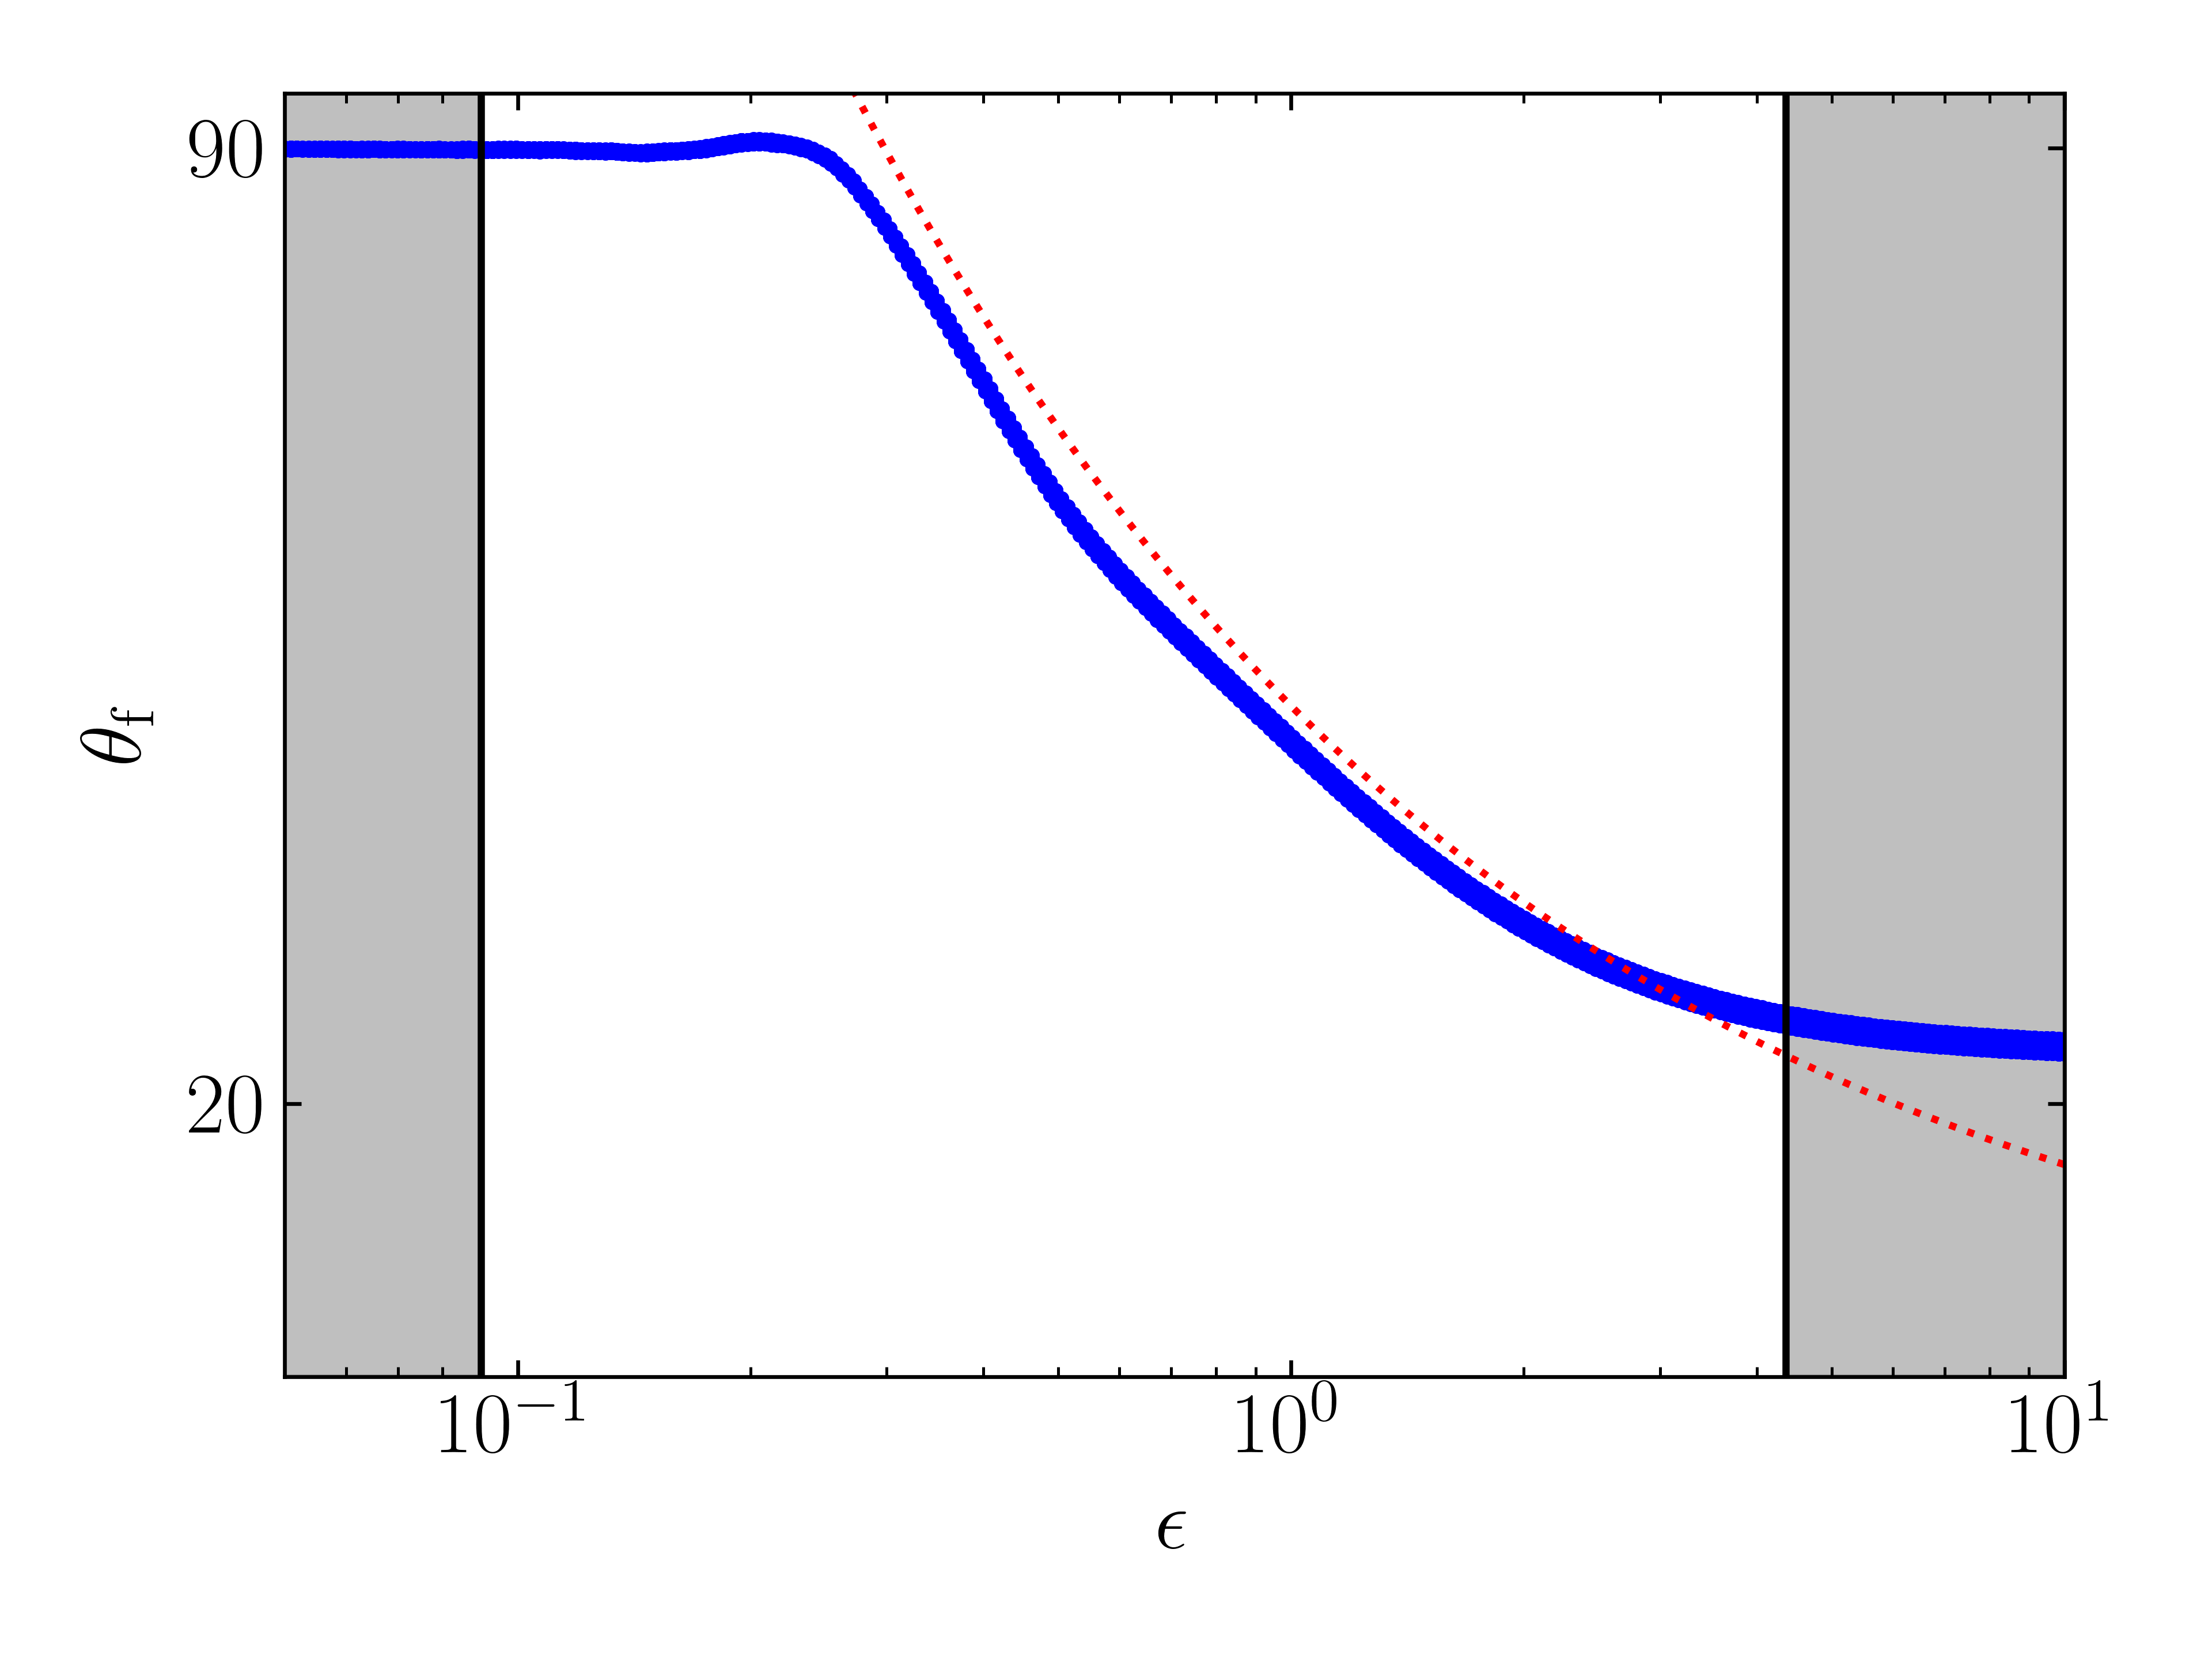
\includegraphics[width=0.5\textwidth]{../initial/2_toy2/3scan_20.png}
    \caption{Same as Fig.~\ref{fig:nonad_3_scan} but for $I=20^\circ$. Note that
    Eq.~\eqref{eq:nonad_q_f} is accurate until $\theta_{\rm f} \approx 90^\circ$,
    which is much closer to the transition to adiabaticity. Comparison with
    Fig.~\ref{fig:nonad_3_scan} suggests that the breakdown of
    Eq.~\eqref{eq:nonad_q_f} indeed is caused by the breakdown of the
    non-adiabatic assumption.}\label{fig:nonad_3_scan_20}
\end{figure}

\section{Summary and Discussion}\label{s:disc}

In this paper, we have studied the excitation of planetary obliquities by a
dissipating protoplanetary disk for arbitrary initial misalignment angles. This
is described by transfer function $\theta_{\rm f}\p{\theta_{\rm sd, i}}$, where
$\theta_{\rm f}$ is the final planetary obliquity and $\theta_{\rm sd, i}$ is
the initial misalignment angle between the planet's spin axis and the disk's
orbital angular momentum. We have presented analytical results that capture the
behavior of $\theta_{\rm f}\p{\theta_{\rm sd, i}}$ in both the adiabatic and
nonadiabatic
limits:
\begin{enumerate}
    \item In the adiabatic limit, we are able to reproduce the known result
        $\theta(0) \approx 90^\circ$ \citep{millholland_disk}. We demonstrate
        via numerical simulation the dual-valued behavior of $\theta$ as nonzero
        values of $\theta_{\rm sd, i}$ are permitted (see
        Fig.~\ref{fig:ad_ensemble}). We are able to capture both the exact final
        $\theta$ values and the probabilities of observing each value via
        careful accounting of enclosed phase space area and separatrix crossing
        dynamics \citep{henrard1982,henrard1987}.

    \item As the system transitions more abruptly, the adiabatic prediction
        breaks down when criterion Eq.~\eqref{eq:ad_constr} is violated. We find a
        broad range of $\theta$ values can be excited for a given $\theta_{\rm
        sd, i}$ (see Fig.~\ref{fig:nonad_3_ensemeble}). We provide an analytical
        expression of the bounds on $\theta_{\rm f}\p{\theta_{\rm sd, i}}$ in
        Eq.~\eqref{eq:nonad_q_f_dist}.
\end{enumerate}

It is of interest to note the leading order behavior of $\theta$ in the small
$\theta_{\rm sd, i}$ limit given by Eq.~\eqref{eq:qf_21_approx} and
Eq.~\eqref{eq:qf_23_approx}. Therefore, if $\theta_{\rm sd, i}$ is generally
small, as might be expected for planets that do not experience strong collisions
or scattering, resonance capture induced by an adiabatically dissipating
protoplanetary disk is expected to significantly narrow the final $\theta$
spread compared to the initial $\theta_{\rm sd, i}$ spread.

\bibliographystyle{mnras}
\bibliography{Su_sep_cross}

% \clearpage
% \onecolumn
\appendix

\section{Cassini State Local Dynamics}\label{s:local_dynamics}

In this section, we perform local linearizations about the CSs to determine the
stability of each CS and, when stable, the local libration frequencies.

\subsection{Canonical Equations of Motion and Solutions}

For analytical work, we adopt spherical coordinate system where $\uv{l} =
\uv{z}$ and $\theta, \phi$ are the polar and azimuthal angle of $\uv{s}$. By
convention, we choose $\uv{l}_{\rm z}$ at coordinates $\theta = I, \phi = \pi$.
Note that $\p{\cos \theta, \phi}$ form a canonically conjugate pair of variables
describing $\uv{s}$. To derive equations of motion for these canonical
coordinates, we rewrite Eq.~\eqref{eq:H}
\begin{equation}
    \mathcal{H}\p{\theta, \phi} = -\frac{1}{2}\cos^2\theta
            + \eta \p{\cos \theta \cos I - \sin I \sin \theta \cos \phi}.
\end{equation}

The equations of motion follow by taking derivatives of $\mathcal{H}$ and agree
with Eq.~\eqref{eq:dsdt_base}:
\begin{subequations}\label{se:H_eom}
    \begin{align}
        \rd{\phi}{t} = \pd{\mathcal{H}}{(\cos\theta)}
            &= -\cos\theta + \eta\p{\cos I + \sin I \cot \theta \cos \phi},
                \label{seq:H_eom_phi_t}\\
        \rd{(\cos \theta)}{t} = -\pd{\mathcal{H}}{\phi}
            &= -\eta \sin I \sin \theta \sin \phi.
                \label{seq:H_eom_mu_t}
    \end{align}
\end{subequations}
While these equations are numerically stiff owing to the $\cot\theta$ term, they
are the most intuitive description for analytical work.

We next develop some approximate forms for the CS obliquities that will be
useful for guiding later discussion. Denote $\theta_{\rm cs}$ the obliquity of
some Cassini State (fixed point of Eqs.~\eqref{se:H_eom}).
\begin{enumerate}
    \item $\eta \ll 1, \cos \theta_{\rm cs} \ll 1$ --- This is the limiting case
        for CS2 and CS4 when $\eta \ll \eta_{\rm c}$. We examine
        Eqs.~\eqref{seq:H_eom_phi_t} and approximate $\cot \theta \approx \cos
        \theta$ to find
        \begin{equation}
            \cos \theta_{\rm cs} \approx \frac{\eta \cos I}
                {1 \mp \eta \sin I}.
        \end{equation}
        The two signs correspond to choices of $\cos \phi$. Each sign
        corresponds to one of CS2 and CS4.

    \item $\sin \theta_{\rm cs} \ll 1$ --- The $\eta \ll 1, \eta \gg 1$ cases
        can be solved together, and are the limiting cases both for CS1 and CS3
        when $\eta \ll \eta_{\rm c}$, and for CS2 and CS3 when $\eta \gg
        \eta_{\rm c}$. It proves easiest to rewrite Eqs.~\eqref{seq:H_eom_phi_t}
        as
        \begin{equation}
            0 = \cos \theta_{\rm cs}\p{-1 + 2\eta
                \frac{\sin \p{I \pm \theta_{\rm cs}}}{\sin \p{2\theta_{\rm
                    cs}}}}.\label{eq:rewritten_dphi}
        \end{equation}
        The $\pm$ choice again comes from choice of $\cos \phi$. Then assuming
        $\theta_{\rm cs}, I \ll 1$, we obtain $\frac{I \pm
        \theta_{\rm cs}}{2\theta_{\rm cs}} = \frac{1}{2\eta}$ or
        \begin{equation}
            \theta_{\rm cs} = \frac{\eta I}{1 \mp \eta}.
        \end{equation}

        In the limit $\eta \ll \eta_{\rm c}$, these two solutions describe CS1
        and CS3, while in the limit $\eta \gg \eta_{\rm c}$ these two solutions
        describe CS2 and CS3.
\end{enumerate}
Note that the $\theta_{\rm cs}$ values derived here do not follow the same
convention as Fig.~\ref{fig:cs_locs}, because the previous $\theta$ conventions
presume $\cos \phi = -1$ for all states and let $-\pi \leq \theta < \pi$.

\subsection{Stability and Frequency of Local Oscillations}\label{ss:eigens}

To examine stability of each CS, it proves very easy to handle them generally.
We linearize about an equilibrium located at $\phi_{\rm cs} = 0, \pi$ but
arbitrary $\theta_{\rm cs}$. Linearizing Eqs.~\eqref{se:H_eom} about $\phi =
\phi_{\rm cs} + \delta \phi, \theta = \theta_{\rm cs} + \delta \theta$ gives
\begin{subequations}\label{se:H_eom_lin}
    \begin{align}
        \rd{\delta \phi}{t} &= \sin \theta_{\rm cs} \delta \theta
            \mp \eta \frac{\sin I}{\sin^2\theta_{\rm cs}} \delta \theta,\\
        \rd{\delta \theta}{t} &= \pm \eta \sin I \delta \phi.
    \end{align}
\end{subequations}
Note that the positive sign corresponds to $\phi_{\rm cs} = 0$. Eliminating
$\delta \theta$ gives
\begin{align}
    \rtd{\delta \phi}{t} &= \p{\sin \theta_{\rm cs}
        \mp \eta \sin I\csc^2\theta}\p{\pm \eta \sin I} \delta
            \phi,\\
        &\equiv \lambda^2\delta \phi.\label{eq:lambda2}
\end{align}
A plot of $\lambda^2$ for each of the CSs is given in Fig.~\ref{fig:lambda2}.
From the plot, it is clear that only CS4 is a saddle point, while the other
three are centers (stable). The local libration frequency for these points is
just
\begin{align}
    \omega_{\rm lib} &= \sqrt{-\lambda^2},\\
        &= \sqrt{\p{\sin \theta_{\rm cs}
            \mp \eta \sin I \csc^2\theta}\p{\mp \eta \sin I}}.
\end{align}
The libration period is related simply $T_{\rm lib} = \frac{2\pi}{\omega_{\rm
lib}}$.
\begin{figure}[t]
    \centering
    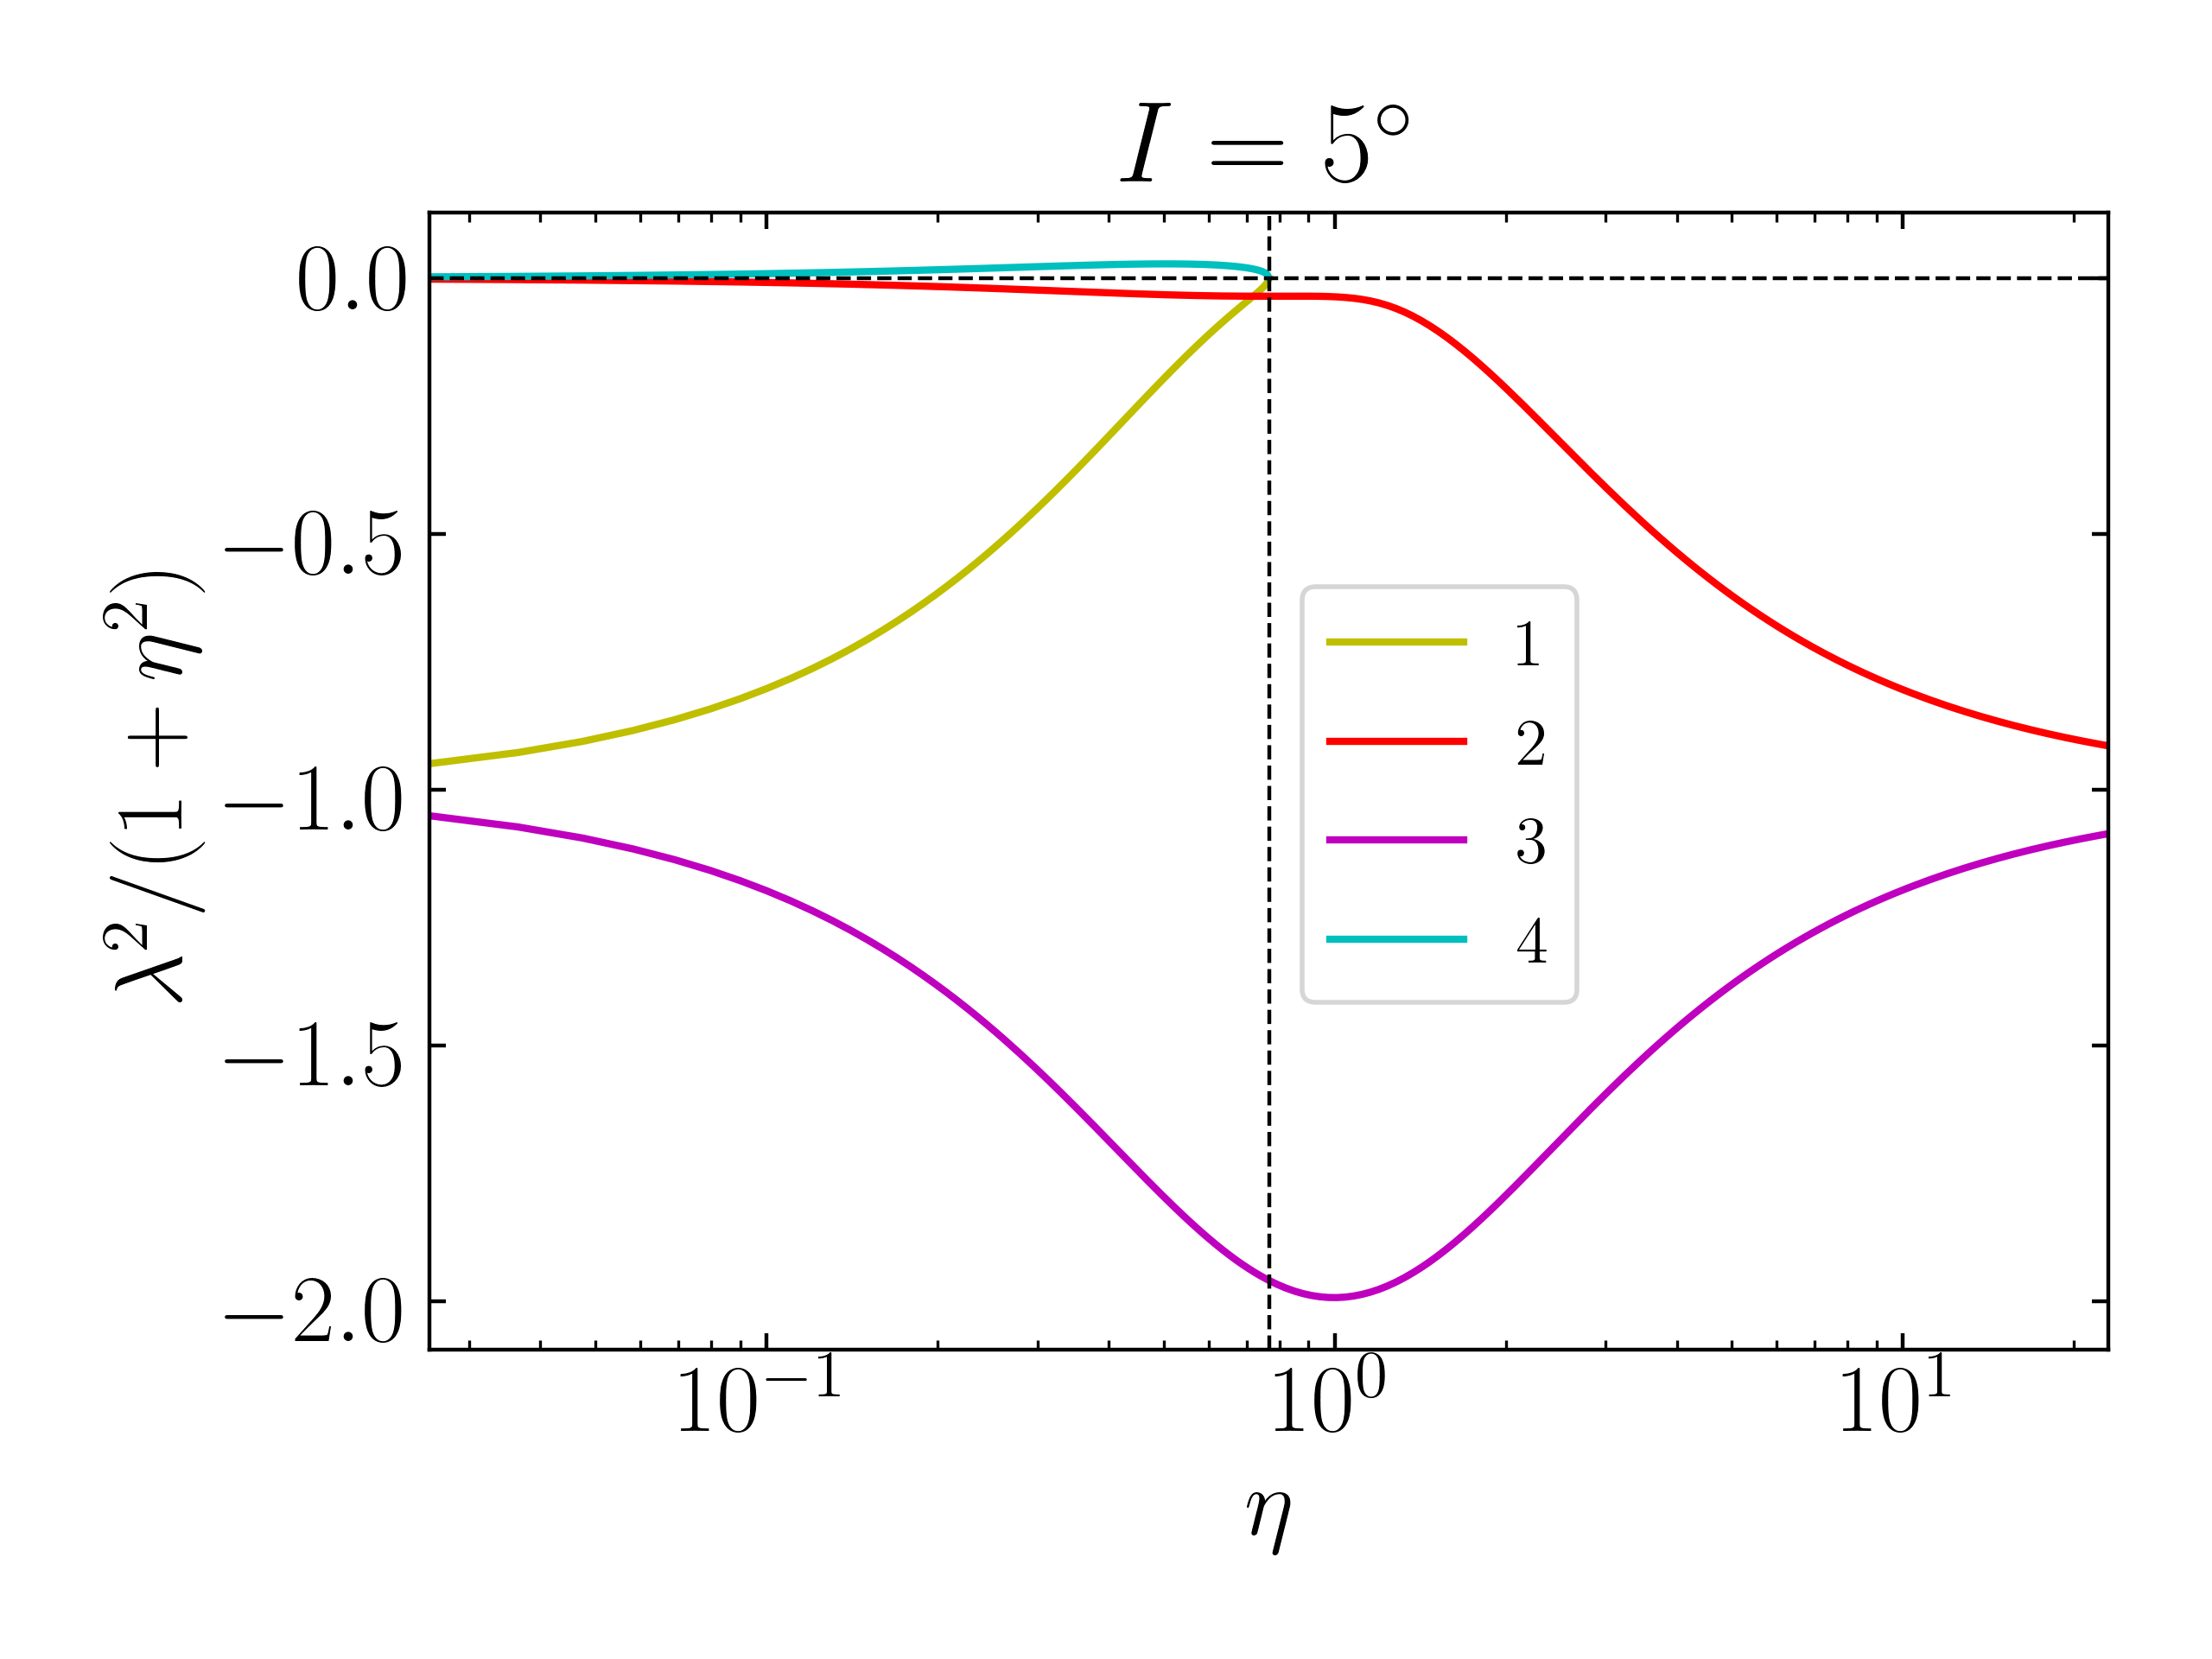
\includegraphics[width=0.5\textwidth]{../initial/99_misc/2_lambdas.png}
    \caption{Plot of $\lambda^2$ per Eq.~\eqref{eq:lambda2} evaluated at each
    of the Cassini States. The vertical axis is rescaled to limit the vertical
    extent of the plot. Note that CS4 is a saddle point ($\lambda^2 > 0$) when
    it exists while all others are centers ($\lambda^2 < 0$). The horizontal
    dashed line is $\lambda^2 = 0$ the instability boundary while $\eta_{\rm c}$ is
    labered in the vertical dashed line.}\label{fig:lambda2}
\end{figure}

Note that our expression is somewhat more complicated than in existing
literature \citep{millholland_disk,ward2004II}. This seems to stem from the
approximation $\theta \gg I$ made in deriving Equation 3 of
\citet{ward2004II}. This is invalid in the $\eta \gtrsim \eta_{\rm c}$ limit for
CS2, since $\theta_{\rm cs} \approx I$ in this regime as was shown above.

\section{Approximate Adiabatic Evolution}\label{s:ad_approx}

In this section, we will use approximations valid for small $\eta$ to derive
analytic expressions for the final obliquities at small $\theta_{\rm sd, i}$ and
associated probabilities for the II $\to$ I and II $\to$ III tracks that are
accessible.

We first seek a simple parameterization for the separatrix. We first solve for
equilibria of the equation of motion Eq.~\eqref{eq:dsdt_base} to compute the
coordinates for Cassini State 4:
\begin{equation}
    \cos \theta_4 \approx \frac{\mu \cos I}{1 - \eta \sin I}.
\end{equation}
Note that $\phi_4 = 0$. Then, the separatrix is the level curve of the
Hamiltonian intersecting CS4, so it satisfies $\mathcal{H}\p{\theta_{\rm
sep}(\phi), \phi} = \mathcal{H}\p{\theta_4, \phi_4}$. This solves to be
approximately
\begin{equation}
    \cos \theta_{\rm sep}(\phi) \approx \cos \theta_4 \pm
        \sqrt{2\eta \sin I\p{1 - \cos \phi}}.
\end{equation}
Integration of the phase area enclosed by the two legs of the separatrix then
yields
\begin{equation}
    A_{\rm II}(\eta) \approx 16\sqrt{\eta \sin I}.\label{eq:a_approx}
\end{equation}
This, in conjunction with Eq.~\eqref{eq:henrard_hop}, is sufficient to compute
$\theta_{\rm f}\p{\theta_{\rm sd, i}}$ for zone II initial conditions.

\begin{enumerate}
    \item For a given $\theta_{\rm sd, i}$, we know that if $\eta \to \infty$
        then the trajectory executes simple libration about $\uv{l}_{\rm d}$,
        and so $A = 2\pi\p{1 - \cos \theta_{\rm sd, i}} \approx \pi \theta_{\rm
        sd, i}^2$. This then implies $\eta_\star$ must be the solution to
        $A_{\rm II}(\eta_\star) = A$, or
        \begin{align}
            \eta_\star &\approx \p{\frac{2\pi\p{1 - \cos \theta_{\rm sd,i}}}{
                        16}}^2 / \sin I,\\
                    &\approx \p{\frac{\pi \theta_{\rm sd, i}^2}{16}}^2/\sin I.
        \end{align}

    \item Upon separatrix encounter, a transition to either zone I or zone
        III occurs. These can be calculated to have associated probabilities
        (using the approximate area Eq.~\eqref{eq:a_approx})
        \begin{subequations}
            \begin{align}
                \Pr_{\rm II \Rightarrow I} &\approx \frac{2\pi
                    \eta_{\star} \cos I + 4\sqrt{\eta_{\star}\sin
                    I}}{8\sqrt{\eta_{\star}\sin I}},\\
                \Pr_{\rm II \Rightarrow III} &\approx \frac{-2\pi
                    \eta_{\star} \cos I + 4\sqrt{\eta_{\star}\sin
                    I}}{8\sqrt{\eta_{\star}\sin I}}.
            \end{align}
        \end{subequations}

    \item Upon a transition to zone I or zone III, the final obliquities can
        be predicted by observing the final adiabatic invariant $A_{\rm f} = -A_{\rm
        I}(\eta_\star)$ in the zone I case and $A_{\rm f} = A_{\rm I}(\eta_\star) +
        A_{\rm I}I(\eta_\star)$ in the zone III case. As $\eta \to 0$, these
        correspond to obliquities
        \begin{subequations}\label{se:q_f_approx}
            \begin{align}
                \cos \theta_{\rm f, II \Rightarrow I} &\approx
                    \p{\frac{\pi \theta_{\rm sp, i}^2}{16}}^2 \cot I
                        + \frac{\theta_{\rm sp, i}^2}{4},\\
                \cos \theta_{\rm f, II \Rightarrow III} &\approx
                    \p{\frac{\pi \theta_{\rm sp, i}^2}{16}}^2 \cot I
                        - \frac{\theta_{\rm sp, i}^2}{4}.
            \end{align}
        \end{subequations}
        These are the black dotted lines overplotted in
        Fig.~\ref{fig:ad_ensemble}.
\end{enumerate}

\section{Derivation of Nonadiabatic Evolution}\label{s:nonad_app}

We present a single result, the derivation of Eq.~\eqref{eq:nonad_q_f}. We take
Eq.~\eqref{eq:dsdt_base} and choose coordinate axes such that $\uv{l} = \uv{z},
\uv{l}_{\rm d} = \uv{z} \cos I + \uv{x}\sin I$, then we obtain
\begin{equation}
    \rd{\uv{s}}{t} = \s{
        \p{\eta \cos I - 1}\uv{z} + \eta \sin I \uv{x}} \times \uv{s}.
\end{equation}

Now, let's assume that $s_{\rm z} \approx \cos I$ throughout the evolution of
$\uv{s}$ (note that $\theta_{\rm sd, i} = 0$ implies the initial $s_{\rm z} = \cos
I$). Then let's examine the evolution of quantity $S = s_{\rm x} + is_{\rm y}$ instead:
\begin{equation}
    \rd{S}{t} = i\p{\eta\cos I - 1}S - i \eta \sin I\cos I.\label{eq:nonad_ode}
\end{equation}
Now this is a first-order ODE in $S$, albeit complex, which can be solved via
an integrating factor
\begin{align}
    \Phi(t) &\equiv \int_{-\infty}^t \p{1 - \eta(t') \cos I}
        \mathrm{d}t',\\
    \at{S(t) e^{i\Phi(t)}}_{-\infty}^t
        &= \int\limits_{-\infty}^t e^{i\Phi(t')}
            \p{-i\eta(t')\sin I\cos I}\;\mathrm{d}t'\label{eq:nonad_int}
\end{align}
We now invoke stationary phase, asserting that $e^{i\Phi(t)}$ is dominated by
its contribution where $\dot{\Phi} = 0$ (the phases add constructively). But
$\dot{\Phi} = 0$ is where $1 - \eta\cos I = 0$, or where $\eta\cos I = 1$.

Now at this point, let's choose $\eta(0) = 1/\cos I, \at{\rd{\eta}{t}}_{t=0} =
-\epsilon/\cos I$. Then we expand near $t = 0$ so
\begin{align}
    \Phi(t) &\approx \Phi(0) + \frac{1}{2}\ddot{\Phi}t^2,\\
        &\approx \Phi(0) + \frac{1}{2}\epsilon t^2,\\
    \int\limits_{-\infty}^t e^{i\Phi(t')}\eta(t')\;\mathrm{d}t'
        &\approx
        \begin{cases}
            0 & t < 0,\\
            \frac{1}{\cos I}e^{i\Phi(0)}\int\limits_{-\infty}^\infty
                \exp\s{\frac{i}{2}\epsilon t^2}\;\mathrm{d}t
                & t > 0.
        \end{cases}\\
    \int\limits_{-\infty}^\infty
                \exp\s{\frac{i}{2}\epsilon t^2}\;\mathrm{d}t
        &= \int\limits_{-\infty}^\infty e^{-\tau^2}\;\mathrm{d}\tau
            \sqrt{\frac{2}{i\epsilon}},\\
        &= \sqrt{\frac{2\pi}{i\epsilon}}.
\end{align}

Now, it should be noted that $e^{i\Phi}$ is just a phase; all we really care
about is $\abs{S} = \sqrt{1 - s_{\rm z}^2}$. Thus, taking the absolute value of both
sides of Eq.~\eqref{eq:nonad_int}, assuming $S\p{-\infty} \ll S\p{+\infty}$ and
noting $\theta_{\rm f} \approx \abs{S}(+\infty)$, we obtain
\begin{equation}
    \theta_{\rm f} = \tan I\cos I\sqrt{\frac{2\pi}{\epsilon}}.
        \label{eq:nonad_dong}
\end{equation}

We note the resemblance to a similar result given by \citet{malhotra_calc}
describing the impact of a secular resonance sweeping through a system. Both
results have the scaling with repsect to $\epsilon$, despite the vastly
different calculation.

It should be noted that this result breaks down in two ways:
\begin{enumerate}
    \item If the evolution of $\uv{s}$ is adiabatic, then it is invalid to
        assume $s_{\rm z}$ is approximately constant in time, as many
        circulation/libration orbits can ensue. Only when the driving is
        sufficiently impulsive that the evolution dominates the change in
        $s_{\rm z}$
        is this calculation valid.

    \item If $\abs{S\p{-\infty}} \sim \abs{S\p{+\infty}}$, then taking the
        absolute value of both sides of Eq.~\eqref{eq:nonad_int} no longer
        simply yields $\abs{S}\p{+\infty}$. This corresponds to the extreme
        limit where $\eta$ changes so suddenly that $\uv{s}$ has no time to
        respond and remains roughly unchanged as $\eta \to 0$. This is
        accommodated by noting $\theta_{\rm f} \geq \theta_{\rm sd, i}$, so the
        correct estimate can be roughly amended
        \begin{equation}
            \theta_{\rm f} \simeq \min\p{\tan I\cos
                I\sqrt{\frac{2\pi}{\epsilon}}, \theta_{\rm sd, i}}.
        \end{equation}
\end{enumerate}

\bsp
\label{lastpage} % chktex 24
\end{document}
